\documentclass[uplatex, dvipdfmx]{jsreport}
    
\title{ComputerとLogic}
\author{司馬博文 J4-190549\\hirofumi-shiba48@g.ecc.u-tokyo.ac.jp}
\date{\today}
\pagestyle{headings} \setcounter{secnumdepth}{4}
\usepackage{amsmath, amsfonts, amsthm, amssymb, ascmac, color, comment, wrap fig}

\usepackage{mathtools}
\mathtoolsset{showonlyrefs=true} %labelを附した数式にのみ附番される.

\usepackage{tikz, tikz-cd}
\usepackage[all]{xy}
\def\objectstyle{\displaystyle} %デフォルトではxymatrix中の数式が文中数式モードになるので,それを直した.

%化学式をTikZで簡単に書くためのパッケージ.
\usepackage[version=4]{mhchem} %texdoc mhchem
%化学構造式をTikZで描くためのパッケージ.
\usepackage{chemfig}
%IS単位を書くためのパッケージ
\usepackage{siunitx}
%取り消し線を引くためのパッケージ
\usepackage{ulem}

%\rotateboxコマンドを,文字列の中心で回転させるオプション.
%他rotatebox, scalebox, reflectbox, resizeboxなどのコマンド.
\usepackage{graphicx}

%加藤晃史さんがフル活用していたtcolorboxを,途中改ページ可能で.
\usepackage[breakable]{tcolorbox}

%enumerate環境を凝らせる.
\usepackage{enumerate}

%日本語にルビをふる
\usepackage{pxrubrica}

%足助さんからもらったオプション
%\usepackage[shortlabels,inline]{enumitem}
%\usepackage[top=15truemm,bottom=15truemm,left=10truemm,right=10truemm]{geometry}

%以下,ソースコードを表示する環境の設定.
\usepackage{listings,jvlisting} %日本語のコメントアウトをする場合jlistingが必要
%ここからソースコードの表示に関する設定
\lstset{
  basicstyle={\ttfamily},
  identifierstyle={\small},
  commentstyle={\smallitshape},
  keywordstyle={\small\bfseries},
  ndkeywordstyle={\small},
  stringstyle={\small\ttfamily},
  frame={tb},
  breaklines=true,
  columns=[l]{fullflexible},
  numbers=left,
  xrightmargin=0zw,
  xleftmargin=3zw,
  numberstyle={\scriptsize},
  stepnumber=1,
  numbersep=1zw,
  lineskip=-0.5ex
}
%lstlisting環境で,[caption=hoge,label=fuga]などのoptionを付けられる.
\makeatletter
    \AtBeginDocument{
    \renewcommand*{\thelstlisting}{\arabic{chapter}.\arabic{section}.\arabic{lstlisting}}
    \@addtoreset{lstlisting}{section}
    }
\makeatother
%caption番号を「[chapter番号].[section番号].[subsection番号]-[そのsubsection内においてn番目]」に変更
\renewcommand{\lstlistingname}{program}
%caption名を"program"に変更

%%%
%%%フォント
%%%

%本文・数式の両方のフォントをTimesに変更するお手軽なパッケージだが,LaTeX標準数式記号の\jmath, \amalg, coprodはサポートされない.
% \usepackage{mathptmx}
%Palatinoの方が完成度が高いと美文書作成に書いてあった.
\usepackage[sc]{mathpazo} %オプションは,familyの指定.pplxにしている.
%2000年のYoung Ryuによる新しいTimes系.なおPalatinoもある.
% \usepackage{newtxtext, newtxmath}
%拡張数学記号.\textsectionでブルバキに!
\usepackage{textcomp, mathcomp}
\usepackage[T1]{fontenc} %8bitエンコーディングにする.comp系拡張数学文字の動作が安定する.
%AMS Euler.Computer Modernと相性が悪いとは…….
\usepackage{ccfonts, eulervm} %KnuthのConcrete Mathematicsの組み合わせ.
% \renewcommand{\rmdefault}{pplx} %makes LaTeX use Palatino in place of CM Roman.Do not use the Euler math fonts in conjunction with the default Computer Modern text fonts – this is ugly!

%%% newcommands
    %参考文献で⑦というのを出したかった.\circled{n}と打てば良い.LaTeX StackExchangeより.
\newcommand*\circled[1]{\tikz[baseline=(char.base)]{\node[shape=circle,draw,inner sep=0.8pt] (char) {#1};}}

%%%
%%% ショートカット 足助さんからのコピペ
%%%

\DeclareMathOperator{\grad}{\mathrm{grad}}
\DeclareMathOperator{\rot}{\mathrm{rot}}
\DeclareMathOperator{\divergence}{\mathrm{div}}
\newcommand\R{\mathbb{R}}
\newcommand\N{\mathbb{N}}
\newcommand\C{\mathbb{C}}
\newcommand\Z{\mathbb{Z}}
\newcommand\Q{\mathbb{Q}}
\newcommand\GL{\mathrm{GL}}
\newcommand\SL{\mathrm{SL}}
\newcommand\False{\mathrm{False}}
\newcommand\True{\mathrm{True}}
\newcommand\tr{\mathrm{tr}}
\newcommand\M{\mathcal{M}}
\newcommand\F{\mathbb{F}}
% \newcommand\H{\mathbb{H}} すでにある.
\newcommand\id{\mathrm{id}}
\newcommand\A{\mathcal{A}}
%\renewcommand\coprod{\rotatebox[origin=c]{180}{$\prod$}}
\newcommand\pr{\mathrm{pr}}
\newcommand\U{\mathfrak{U}}
\newcommand\Map{\mathrm{Map}}
\newcommand\dom{\mathrm{dom}}
\newcommand\cod{\mathrm{cod}}
\newcommand\supp{\mathrm{supp}}
%%% 複素解析学
\renewcommand\Re{\mathrm{Re}\;}
\renewcommand\Im{\mathrm{Im}\;}
\newcommand\Gal{\mathrm{Gal}}
\newcommand\PGL{\mathrm{PGL}}
\newcommand\PSL{\mathrm{PSL}}
%%% 解析力学
\newcommand\x{\mathbf{x}}
\newcommand\q{\mathbf{q}}
%%% 集合と位相
\newcommand\ORD{\mathrm{ORD}}

%%% 圏
\newcommand\Hom{\mathrm{Hom}}
\newcommand\Mor{\mathrm{Mor}}
\newcommand\Aut{\mathrm{Aut}}
\newcommand\End{\mathrm{End}}
\newcommand\op{\mathrm{op}}
\newcommand\ev{\mathrm{ev}}
\newcommand\Ob{\mathrm{Ob}}
\newcommand\Ar{\mathrm{Ar}}
\newcommand\Arr{\mathrm{Arr}}
\newcommand\Set{\mathrm{Set}}
\newcommand\Grp{\mathrm{Grp}}
\newcommand\Cat{\mathrm{Cat}}
\newcommand\Mon{\mathrm{Mon}}
\newcommand\CMon{\mathrm{CMon}}
\newcommand\Pos{\mathrm{Pos}}
\newcommand\Vect{\mathrm{Vect}}
\newcommand\FinVect{\mathrm{FinVect}}
\newcommand\Fun{\mathrm{Fun}}
\newcommand\Ord{\mathrm{Ord}}

%%%
%%% 定理環境 以下足助さんからのコピペ
%%%

\newtheoremstyle{StatementsWithStar}% ?name?
{3pt}% ?Space above? 1
{3pt}% ?Space below? 1
{}% ?Body font?
{}% ?Indent amount? 2
{\bfseries}% ?Theorem head font?
{\textbf{.}}% ?Punctuation after theorem head?
{.5em}% ?Space after theorem head? 3
{\textbf{\textup{#1~\thetheorem{}}}{}\,$^{\ast}$\thmnote{(#3)}}% ?Theorem head spec (can be left empty, meaning ‘normal’)?
%
\newtheoremstyle{StatementsWithStar2}% ?name?
{3pt}% ?Space above? 1
{3pt}% ?Space below? 1
{}% ?Body font?
{}% ?Indent amount? 2
{\bfseries}% ?Theorem head font?
{\textbf{.}}% ?Punctuation after theorem head?
{.5em}% ?Space after theorem head? 3
{\textbf{\textup{#1~\thetheorem{}}}{}\,$^{\ast\ast}$\thmnote{(#3)}}% ?Theorem head spec (can be left empty, meaning ‘normal’)?
%
\newtheoremstyle{StatementsWithStar3}% ?name?
{3pt}% ?Space above? 1
{3pt}% ?Space below? 1
{}% ?Body font?
{}% ?Indent amount? 2
{\bfseries}% ?Theorem head font?
{\textbf{.}}% ?Punctuation after theorem head?
{.5em}% ?Space after theorem head? 3
{\textbf{\textup{#1~\thetheorem{}}}{}\,$^{\ast\ast\ast}$\thmnote{(#3)}}% ?Theorem head spec (can be left empty, meaning ‘normal’)?
%
\newtheoremstyle{StatementsWithCCirc}% ?name?
{6pt}% ?Space above? 1
{6pt}% ?Space below? 1
{}% ?Body font?
{}% ?Indent amount? 2
{\bfseries}% ?Theorem head font?
{\textbf{.}}% ?Punctuation after theorem head?
{.5em}% ?Space after theorem head? 3
{\textbf{\textup{#1~\thetheorem{}}}{}\,$^{\circledcirc}$\thmnote{(#3)}}% ?Theorem head spec (can be left empty, meaning ‘normal’)?
%
\theoremstyle{definition}
 \newtheorem{theorem}{定理}[section]
 \newtheorem{axiom}[theorem]{公理}
 \newtheorem{corollary}[theorem]{系}
 \newtheorem{proposition}[theorem]{命題}
 \newtheorem*{proposition*}{命題}
 \newtheorem{lemma}[theorem]{補題}
 \newtheorem*{lemma*}{補題}
 \newtheorem*{theorem*}{定理}
 \newtheorem{definition}[theorem]{定義}
 \newtheorem{example}[theorem]{例}
 \newtheorem{notation}[theorem]{記法}
 \newtheorem*{notation*}{記法}
 \newtheorem{assumption}[theorem]{仮定}
 \newtheorem{question}[theorem]{問}
 \newtheorem{counterexample}[theorem]{反例}
 \newtheorem{reidai}[theorem]{例題}
 \newtheorem{problem}[theorem]{問題}
 \newtheorem*{solution*}{\bf{[解]}}
 \newtheorem{discussion}[theorem]{議論}
 \newtheorem{remark}[theorem]{注}
 \newtheorem{universality}[theorem]{普遍性} %非自明な例外がない.
 \newtheorem{universal tendency}[theorem]{普遍傾向} %例外が有意に少ない.
 \newtheorem{hypothesis}[theorem]{仮説} %実験で説明されていない理論.
 \newtheorem{theory}[theorem]{理論} %実験事実とその(さしあたり)整合的な説明.
 \newtheorem{fact}[theorem]{実験事実}
 \newtheorem{model}[theorem]{模型}
 \newtheorem{explanation}[theorem]{説明} %理論による実験事実の説明
 \newtheorem{anomaly}[theorem]{理論の限界}
 \newtheorem{application}[theorem]{応用例}
 \newtheorem{method}[theorem]{手法} %実験手法など,技術的問題.
 \newtheorem{history}[theorem]{歴史}
 \newtheorem{research}[theorem]{研究}
% \newtheorem*{remarknonum}{注}
 \newtheorem*{definition*}{定義}
 \newtheorem*{remark*}{注}
 \newtheorem*{question*}{問}
 \newtheorem*{axiom*}{公理}
 \newtheorem*{example*}{例}
%
\theoremstyle{StatementsWithStar}
 \newtheorem{definition_*}[theorem]{定義}
 \newtheorem{question_*}[theorem]{問}
 \newtheorem{example_*}[theorem]{例}
 \newtheorem{theorem_*}[theorem]{定理}
 \newtheorem{remark_*}[theorem]{注}
%
\theoremstyle{StatementsWithStar2}
 \newtheorem{definition_**}[theorem]{定義}
 \newtheorem{theorem_**}[theorem]{定理}
 \newtheorem{question_**}[theorem]{問}
 \newtheorem{remark_**}[theorem]{注}
%
\theoremstyle{StatementsWithStar3}
 \newtheorem{remark_***}[theorem]{注}
 \newtheorem{question_***}[theorem]{問}
%
\theoremstyle{StatementsWithCCirc}
 \newtheorem{definition_O}[theorem]{定義}
 \newtheorem{question_O}[theorem]{問}
 \newtheorem{example_O}[theorem]{例}
 \newtheorem{remark_O}[theorem]{注}
%
\theoremstyle{definition}
%
\raggedbottom
\allowdisplaybreaks

%証明環境のスタイル
\everymath{\displaystyle}
\renewcommand{\proofname}{\bf [証明]}
\renewcommand{\thefootnote}{\dag\arabic{footnote}}	%足助さんからもらった.どうなるんだ?

%mathptmxパッケージ下で,\jmath, \amalg, coprodの記号を出力するためのマクロ.TeX Wikiからのコピペ.
% \DeclareSymbolFont{cmletters}{OML}{cmm}{m}{it}
% \DeclareSymbolFont{cmsymbols}{OMS}{cmsy}{m}{n}
% \DeclareSymbolFont{cmlargesymbols}{OMX}{cmex}{m}{n}
% \DeclareMathSymbol{\myjmath}{\mathord}{cmletters}{"7C}
% \DeclareMathSymbol{\myamalg}{\mathbin}{cmsymbols}{"71}
% \DeclareMathSymbol{\mycoprod}{\mathop}{cmlargesymbols}{"60}
% \let\jmath\myjmath
% \let\amalg\myamalg
% \let\coprod\mycoprod
\begin{document}
\tableofcontents

\part{論理と集合}

\chapter{一階論理の形式化}

まず,数理論理学で扱われる形式である一階述語論理と呼ばれるデータ構造を,帰納的定義により定義する.
その意味論の導入方法を,モデルを介して接続する.
意味論と構文論とは,形式体系と数学の理論体系との対立・相互関係のことを特にこう呼ぶ.
2つの密接な結び付きは健全性と完全性に端的に集約される.健全性とは証明可能な論理式が常に正しい$\rightarrow$ことを主張し,
完全性が正しい論理式が証明可能である$\leftarrow$ことを主張する.

すると,一階の論理式には,意味論的な振る舞いを全く同一にするという意味で標準形が見つかる.
次の形をした論理式はSkolem標準形と呼ばれ,その双対概念はHerbrand標準形と呼ばれる.
\[ \forall\vec{x}A(\vec{x};\vec{a}) \]
ここから数理論理学が始まる.

\section{記法}

\begin{enumerate}
    \item $:\Leftrightarrow$は,左辺を右辺で定義すると言うメタ言語内での記法である.
    \item 同様にして,$\Rightarrow$や$\Leftrightarrow$はメタ論理での「ならば」記号として使い,$\to$や$\leftrightarrow$を一階述語論理の論理記号として採用する.
    \item 配置集合は$x^I$とも${}^I\!x$とも書く.
    \item $\langle x_0,\cdots,x_n\rangle$とは,自然数の有限列$(x_0,\cdots,x_n)\in{}^{<\omega}\!\N$を,Cantor写像$J^\infty$により自然数に対応させたもの
    $J^\infty(x_0,\cdots,x_n)=\langle x_0,\cdots,x_n\rangle$である.でも両方とも自然数の列として混用することも多い.
    \item 変数や定数の組を$\vec{x}:=(x_1,\cdots,x_n)$と書き,$\forall\vec{x}$を記号列$\forall x_1\forall x_2\cdots\forall x_n$の略記とする.
\end{enumerate}

\section{集合の扱い,帰納的定義,Cantorの対関数}

\subsection{集合と濃度}

\begin{screen}
形式体系は記号列を扱う.その濃度の議論の基礎を見る.
$\N$は構成子$(0,s)$から帰納的に定まる.その上の有限列$\N$-listも定まる.
従って,可逆な写像$\N^2\to\N$は一意に$\N$-list上に一意に定まる.
このような議論で,結論$\N\simeq{}^{<\omega}\!\N$を得る.
この同型射は計算可能であり,「数え方が存在する」ことを意味する.
その数え方の例(これしか存在しないのだろうか?)$J^\infty$を以下のように構成できる.
\end{screen}

\begin{notation}
    ${}^{<\omega}\!X:=\cup_{n\in\N}X^n$を,集合$X$の元の有限列全体からなる集合とする.
\end{notation}

\begin{definition}[Cantor's pairing function]
    次の関数$J:\N^2\to\N$をCantorの対関数という.
    \[ J(n,m) = \frac{(n+m)(n+m+1)}{2} + m = \left(\sum_{i\le n+m}i\right) + m \]
\end{definition}
\begin{remark}
    自然数の組$(n,m)$を二数の和$n+m$によって分類する.$n+m=k$の時,そのような組は$k+1$個存在する.
    これを最初から番号を付けていき,$n+m=k$のものは全て付け終わったとする.すでに番号は$\sum_{i\le k+1}i$まで付け終わったいる.
    従って,$n+m=k+1$を満たす組$k+2$個は,$m$の値に依って$\sum_{i\le k+1}i+m$と付ければ良い.
    この帰納的定義に定義した関数を明示的に書き下すと,随分と綺麗な形になる.

    逆関数は,この$n+m=k$の値を復元する関数$t:\N\to\N$を定めれば,簡単に構築できる.
\end{remark}

\begin{proposition}\mbox{}\\
    $t(n)=\max\left\{t\le n\;\middle|\; \sum_{i\le t}i\le n\right\}$とする.次の$J_1,J_2$は$J$の逆関数である.
    \begin{align*}
        J_2(n) &= n-\sum_{i\le t(n)}i &J_1(n) &= t(n)-J_2(n)
    \end{align*}
\end{proposition}

\begin{remark}
    $J$を繰り返すことで,$J^n:\N^n\to\N$が次のように定まる.
    \[\xymatrix@C=36pt@R=2.8pt{
        J^n:\N^n \ar[r] & \N \\
        (x_0,x_1,\cdots,x_{n-2},x_{n-1}) \ar@{|->}[r] \ar@{(-}[u] & J(x_0,J(x_1,J(\cdots,J(x_{n-2},x_{n-1})\cdots))) \ar@{(-}[u]
    }\]
    この逆は次のように定まる.
    \[J_i^n(x)=\begin{cases}
        J_1(J_2^{(i)}(x)) &i<n-1の時\\
        J_2^{(n-1)}(x) & i=n-1の時
    \end{cases}\]
\end{remark}

\begin{proposition}\label{prop-cardinality-of-expressions}
    $X$が可算集合ならば,その有限列全体の集合${}^{<\omega}\!X$も可算である.
\end{proposition}
\begin{remark}
    ${}^{<\omega}\!\N$の元を,Cantorの対関数$J$を用いて畳み込んでいく関数を帰納的に定義すれば,
    その閉包${}^{<\omega}\!\N$上に可逆な関数$J^\infty:{}^{<\omega}\!\N\to\N$が定まる.
\end{remark}
\begin{proof}
    次のように構成した写像$J^\infty:{}^{<\omega}\!\N\to\N$は可逆である.
    列の長さ$n$に依って挙動を変えるように,次のように定義すれば良い.
    \[J^\infty(x_0,\cdots,x_{n-1})\begin{cases}
        J(0,0) &n=0のとき\\
        J(0,1+x_0) &n=1のとき\\
        J(n-1,J^n(x_0,\cdots,x_{n-1})) &n>1のとき
    \end{cases}\]
    逆関数は,$x=J^\infty(x_0,\cdots,x_{n-1})$としたとき,まず列の長さの情報を復元する.
    \[length(x)=\begin{cases}
        0 &x=J(0,0)=0のとき\\
        J_1(x)+1 &otherwise
    \end{cases}\]
    これにより,順次$i=0,1,\cdots,n-1$について,次のように復元できる.
    \[x_i=\begin{cases}
        J_2(x)-1 &length(x)=1のとき\\
        J_i^{length(x)}(J_2(x)) &otherwise
    \end{cases}\]
    
    以上の議論は正確には,$J^\infty$の再帰的定義をアルゴリズム的に与えているのみである.
    計算機上に実装してみたい.
\end{proof}

\begin{example}
    $J^\infty(1,0)=J(1,J^2(1,0))=J(1,J(1,0))=J(1,1)=2$
    すごい!計算可能だ.この順番で折りたたんでいくからか!順番って大事だな,順番って関数の本質だな.
    「長さ$n=1$のものだけ先に数えてしまおう」とか言う方針では数え終わらないのだが,問題は数え終わらなさそのもので,
    数え方が存在するかどうかが可算性のポイントなのだな.そして,${}^{<\omega}\!\N$にはこのような数え方$J^\infty$が存在した.
\end{example}

\subsection{二項関係}

\begin{screen}
    形式的な議論をするにあたって,集合の要素に言及する言葉としての,二項述語をいくつか整備しておくと便利である.

    同値関係が一番代表的な二項関係と言える,これは非常に普遍的な言語となる.また,対称的な関係からの同値関係の一般的な構成法として,「反射的推移閉包」が存在する.
    反射推移閉包は射の特徴である.このうち対称的なものを同型(同値関係)というのである.

    順序関係とは,「反対称性と推移性」を持つ二項関係のことである.このままでは共役な2つの関係(反射的閉包と非反射的核)が考えられるが,特に数学では
    反射的なものを順序とする.
\end{screen}

\begin{definition}[二項関係の属性:reflexive, symmetric]\mbox{}
    \begin{enumerate}
        \item $R$が$A$上反射的であるとは,次が成り立つことをいう:$\forall x\in A,\; R(x,x)$.
        \item $R$が$A$上非反射的であるとは,次が成り立つことをいう:$\forall x\in A,\;\lnot R(x,x)$.
        \item $R$が$A$上対称的であるとは,次が成り立つことをいう:$\forall x,y\in A,\;R(x,y)\to R(y,x)$.
        \item $R$が$A$上反対称的であるとは,次が成り立つことをいう:$\forall x,y\in A,\; R(x,y)\land R(y,x)\to x=y$.
        \item $R$が$A$上非対称的であるとは,次が成り立つことをいう:$\forall x,y\in A,\; \lnot(R(x,y)\land R(y,x))$.
    \end{enumerate}
\end{definition}

\subsubsection*{同値関係}

\begin{definition}[同値関係の構成:reflexive and transitive closure]
    関係$R$に対し,その\textbf{推移閉包}$R^+$とは,次のように定義される関係である.
    \begin{enumerate}
        \item $R(x,y)\Rightarrow R^+(x,y)$.
        \item $R^+(x,y)\land R^+(y,z)\Rightarrow R^+(x,z)$.
        \item 上の1,2によって得られるもののみが$R^+$の要素である.
    \end{enumerate}
    関係$R$の\textbf{反射的推移閉包}を,$R^*:=R^+\cup\Delta_X$とする.
\end{definition}

\subsubsection*{順序関係}

特に順序関係について,さらにもう少し言葉を用意する.

順序関係とは,反射性と推移性と反対称性に特徴付けられる二項関係であるが,各順序関係は付随する非反射的な関係を持つ.
実は,命題\ref{prop-reflexive closure}.4が成り立つ.これより,推移性と反対称性の2条件を満たせば順序関係と読んでしまっても差し支えない.
\begin{notation}
    関係$R$に対して,その反射的閉包を$R_=(x,y):\Leftrightarrow R(x,y)\lor x=y$と定める.
    同様にして,非反射的核を$R_\ne(x,y):\Leftrightarrow R(x,y)\land x\ne y$とする.
\end{notation}
\begin{example}
    自然数$\N$上の関係$\subset$は順序関係を定め,$\in=\subset_\ne$がそれに付随する非反射的核である.
\end{example}

\begin{proposition}\label{prop-reflexive closure}\mbox{}
    \begin{enumerate}
        \item 関係$R$が反射的ならば,$(R_\ne)_==R$が成り立つ.
        \item 関係$R$が非反射的ならば,$(R_=)_{\ne}=R$が成り立つ.
        \item $R$が反順序関係ならば,$R_{\ne}$は非対称的かつ推移的な関係である.
        \item $R$が非対称的かつ推移的な関係ならば,$R_=$は半順序関係になる.
    \end{enumerate}
\end{proposition}
\begin{remark}
    これが成り立つのが少し不思議かもしれないが,非反射性と言った時は,条件$\forall x\in A,\; R(x,x)$の否定ではなくて,双対である.
\end{remark}

\begin{definition}[順序の属性:maximum, upper bound, supremum, maximal]
    順序集合$(A,\le)$について,$X\subset A, a\in A$とする.
    \begin{enumerate}
        \item $a$が$X$の\textbf{最大元}であるとは,次が成り立つことをいう:$a\in X\land \forall x\in X,\; x\le a$.
        \item $a$が$X$の\textbf{上界}であるとは,次が成り立つことをいう:$\forall x\in X,\; x\le a$.
        \item $a$が$X$の\textbf{上限}であるとは,$X$の最小の上界であることをいう.
        \item $a$が$X$の\textbf{極大元}であるとは,次が成り立つことをいう:$a\in X\land\forall x\in X,\; a\nless x$.
    \end{enumerate}
    $\nless = \lnot<$が$\ge$と等しくなるのは,これらが全順序を定める時のみである.
    また,双対概念についても,同様に定める.
\end{definition}
\begin{remark}\mbox{}
    \begin{enumerate}
        \item 実数の連続性で,常に上限が存在するという主張は,上界全体の集合$\{ x\in\R \mid \forall a\in X,\; a\le x \}$が下に閉じていることを利用しているに過ぎない.
        つまり,上限という概念装置の定義が巧妙であるだけだ.反射的閉包をここで用いる(?).
        うーん,数は順序関係の極みみたいなデータ構造だが,まだその局所的考察が足りない.
        \item 極大元:「俺より強い奴は居ない」「全員と戦って全勝したわけじゃないが,とりあえず負けたことはない」
    \end{enumerate}
\end{remark}

\begin{definition}[chain, antichain]
    半順序集合$(A,R)$の部分集合$X\subset A$について,$X$が$A$上線型順序(全順序)である時,これを\textbf{A上の鎖}という.
    $X$の任意の二元が比較不能である時:$\forall x,y\in X,\; \lnot(R(x,y)\lor R(y,x))$,これを\textbf{A上の反鎖}という.
\end{definition}

最後に同値関係について考える.関係$R$や関数$f$と両立する/整合的である(compatible)とは,
これらが定める商集合上の同値関係であることとして理解できる.

\subsection{帰納的定義}

\begin{screen}
    帰納的定義はデータ構造の定義に使われる形式手法である.また帰納的定義自体を表すのに,BNF記法というメタ言語がある.
    自然数などの数,多項式などの対象,行列など,扱いたい情報の平方としてのデータ構造は直観的に明らかなものが多いが,
    形式的に厳密に定義するのにこの形式的手法を用いる.すると,その上での関数も,この帰納的な定義から再帰的に定義される.
    これは数学基礎論独特の論理の進め方でもあり,プログラミングをすることも本質的にはこの行為と対応する.
\end{screen}

\begin{definition}[inductive definition]
    集合$A$上での帰納的定義とは,その部分集合$X_0\subset A$と有限個の関数$f:A^n\to A$の組に対して,
    その閉包$X=\cup_{m\in\N}X_m\;\;(X_m:=f(X_{m-1})\;(m=1,2,\cdots))$を$A$上に定義する手法である.この時,$X_0$の元と各関数$(f_i)$を構成子という.
\end{definition}
\begin{remark}
    閉包である点が重要である.後者関数$s:x\mapsto x+1$に対して,組$(0,s)$による帰納的定義は自然数$\N$を定義するが,条件$n\in X\Leftrightarrow n=0\lor\exists m\in X,\; n=m+1$自体は$\Z$も満たす.
    しかしこれらから生成される訳ではない.
\end{remark}
\begin{remark}[多項式]
    整数係数多項式全体の集合$\Z[X]$は次のように定義される.
    \begin{enumerate}
        \item 整数$a\in\Z$は$a\in\Z[X]$で,変数$x\in X$も$x\in\Z[X]$.
        \item $p,q\in\Z[X]$ならば$p+q,p\cdot q\in\Z[X]$.
        \item 以上によって$\Z[X]$に含まれると分かるもののみが$\Z[X]$の元である.
    \end{enumerate}
    $X=\{x_1,\cdots,x_n\}$の時,$p\in\Z[X]$は$p(x_1,\cdots,x_n)$などと書く.

    すると,このデータ構造$\Z[X]$に対する「代入」などの操作が,この帰納的定義から帰納的に定義できることが帰納的に証明できる.
    これが数学者には直観的に明らかなものを形式化する,形式的手法である.
\end{remark}

\subsection{Zornの補題と無限集合の扱い}

無限集合の扱い方は奇妙になることが多く,その際にはZornの補題がどうやら重要な位置を占める.
その理由として,選択公理とZF上同値になることも一つの要因であろう.

\begin{definition}[inductive set]
    順序集合$(A,<)$について,任意の鎖$C\subset A$が上限$\sup C$を$A$上に有する時,$A$は\textbf{帰納的}であるという.
\end{definition}
\begin{lemma}[Zorn's lemma]
    空でない帰納的(半)順序集合は極大元を有する.
\end{lemma}
\begin{remark}\mbox{}
    \begin{enumerate}
        \item 束でも,論理体系についてのコンパクト性定理でも,いろんなデータ構造の上でこのような形をした主張を見てきた.
        Zornの補題も,大域的な性質を,全称命題を使ってではあるが有限の範囲の中で確認可能にする定理の1つであり,しかもこれを順序関係という一番抽象的な述語について行っている.
        この抽象レベルだと,選択公理と同値になるのだ.
        \item 鎖とは,帰納的定義をしたときに$X_m:=f(X_{m-1})\;(m=1,2,\cdots)$が包含関係について作る列である.これが極大元を持つとは,帰納的定義が成功することを意味する.
        そう考えるとなぜこれが成り立つのかの方が不思議になる.反例が作れないのか.ああ,ということは逆に言えば,集合が包含関係について作る順序集合は全て帰納的になるのか.
    \end{enumerate}
\end{remark}

\subsection{有限木の扱い}

\begin{screen}
    木も束も,形式体系では普遍的に現れるデータ構造で,一番おとなしい半順序集合のクラスである.
    特に組み合わせ論的な対象として現れる.
    その中で,有限木$(T,\le)$は,ある自然数の有限列の集合が定める半順序集合$(s(T),\subset)$で
    コード出来(と同型で),
    逆に始切片関係と呼ばれる順序関係について閉じている(推移的である)ような「自然数の有限列の集合」は木とみなせる.
    これは全ての有限木自身が最終的には自然数1つでコード出来ると言う点で数学基礎論的にも重要な事実である.

    従って,木自体も再帰的な方法で定義されるデータ構造であるが,木全体の集合$FinTree\subset P({}^{<\omega}\N)$も再帰的な方法で定義されるデータ構造である.
\end{screen}

\begin{definition}[finite tree]
    有限な半順序集合$(T,\le)$であって,\textbf{根(root)}と呼ばれる最小元$r\in T$を持ち,
    どんな$x\in T$についてもそれ以下の元$(\{y\in T\mid y<x\},\le)$が全順序になっている
    半順序集合$(T,\le,r)$を言う.木の元を\textbf{節(node)}と言う.

    $x<y$であって,$\forall z\in T,\; \lnot(x<z<y)$である時,$y$は$x$の\textbf{子(son, child)}であると言う.
    $son_T(x)\subset T$で$x$の子からなる$T$の元の集合を表す.$son_T(x)=\varnothing$を満たす$x\in T$を\textbf{葉(leaf)}と言う.
\end{definition}
\begin{remark}
    木は$r:tree$と$son:tree^n\to P(tree)$からなる構成子の組$(r,son)$から生成されるデータ構造として定義できる.
\end{remark}

集合${}^{<\omega}\!\N$上に自然に構造を入れて,有限木の受け皿とする.

\begin{definition}[concatenation]
    ${}^{<\omega}\!\N$上の二項演算$*$を,$(x_0,\cdots,x_n)*(y_0,\cdots,y_m)=(x_0,\cdots,x_n,y_0,\cdots,y_m)$として定める.
    多分再帰的方法によっても定められるが,数学の文脈ではあまり見ない.
    同様にして$\varnothing\in{}^{<\omega}\!\N$は見るが,$[]\in{}^{<\omega}\!\N$は見ない.
\end{definition}

\begin{definition}[initial segment]
    ${}^{<\omega}\!\N$上の順序$\subset$を$s\subset (x_0,\cdots,x_{n}):\Leftrightarrow\exists m\le n,\; s=(x_0,\cdots,x_m)$と定める.
    関係$s\subset t$が成り立つ時,$s$は$t$の\textbf{始切片}であると言う.
\end{definition}

\begin{proposition}[有限木の自然数の有限列による表現]
    $(T,\le)$を木とする.次のように帰納的に定めた写像$s:T\to{}^{<\omega}\!\N$は可逆である.
    \begin{enumerate}
        \item $s(r)=\varnothing$
        \item $b\in T$について,$s(b)=(x_0,\cdots,x_{n-1})$であり,$son_T(b)=\{a_1,\cdots,a_m\}$であったとする.
        この時,$s(a_i):=s(b)*(i)\;(i=1,2,\cdots,m)$と定める.
    \end{enumerate}
\end{proposition}
\begin{remark}
    従って,空列を含み,順序$\subset$について閉じている(推移的)であるような${}^{<\omega}\!\N$の有限部分集合は,有限木と同型である.
\end{remark}

\begin{definition}[有限木の自然数によるコード]
    写像$t:LimTree \to \N$次のように帰納的に定義する.ただし$LimTree\subset P({}^{<\omega}\!\N)$は有限木全体の集合とした.
    有限木$T\subset{}^{<\omega}\!\N$に対して,$t(T)\in\N$を次のように定めた$t(T)=t(r)$とする.
    \begin{enumerate}
        \item $son_T(b)=\{a_1,\cdots,a_m\}\;(m\ge 0)$として,$t(b)=J^\infty(b,J^\infty(t(a_1),\cdots,t(a_m)))$と定める.
        子がない場合は$J^\infty(b)$である.
        \item 有限木なので,最終的に$t(r)$が定まる.
    \end{enumerate}
\end{definition}
\begin{remark}
    これは木について拡張できないのか?
\end{remark}
\begin{remark}
    木全体の集合FinTreeも,自然数の列の集合がなすデータ構造として次のように帰納的に定義できる.
    \begin{enumerate}
        \item $\N$の元1つからなる一元集合は木である.
        \item $T_1,\cdots,T_k$は木とする.これらの根$r(T_1),\cdots,r(T_k)$を含む最短の列を$r(T_1),\cdots,r(T_k)\subset r$とし,$son_T(r)=\{r(T_1),\cdots,r(T_k)\}$として作った$T$は木である.
    \end{enumerate}
    $r=[]$としたいから,あまり綺麗な定義ではないな.
\end{remark}

\section{一階述語論理}

\subsection{言語}

\begin{screen}
    一階述語論理での論理式とは,記号の列である.
    論理記号は,一階述語論理と言った時にすでに定まっており,これは論理としての模型である.
    一方非論理記号は,議論の対象に依って様々である.
    殆どの数学分野は一階の量化で十分表現できる.
\end{screen}

\begin{definition}[language]
    次の記号を用意する.
    \textbf{論理記号}または\textbf{論理結合子}は次からなる.
    \begin{enumerate}
        \item (個体変数)$x_1,\cdots,x_n,\cdots$
        \item 結合記号$\land,\lor,\lnot,\to,\leftrightarrow$
        \item 量化記号$\forall,\exists$
        \item 括弧$(),[]$
        \item 等号$=$
    \end{enumerate}
    論理記号以外に,\textbf{非論理記号}からなる集合を$L$と書き,\textbf{言語}と言う.
    数学の分野や用途によって様々であるが,例えば次のようなものがよく登場する.
    \begin{enumerate}
        \item 述語記号$P/n,Q/n,R/n,\cdots$
        \item 関数記号$f/n,g/n,h/n,\cdots$
        \item 定数記号$a,b,c,\cdots$(arity 0の関数記号または述語記号と見なせるが,大抵記号として区別される).
    \end{enumerate}
\end{definition}
\begin{remark}
    $L$は空でも,どんなに大きい集合であっても構わない.また,変数記号は一般に可算無限個用意する.
\end{remark}

\begin{example}[群論]
    群論の言語として$L_G=\{+/2,-/2,-/1,0\}$を定める.$L_G$-文3つからなる集合$T_G$を次のように定め,これを群の公理と呼ぶ.
    \begin{enumerate}
        \item $\forall x\forall y\forall z,\;x+(y+z)=(z+y)+z$,
        \item $\forall x,\; x+0=x$,
        \item $\forall x,\; x-x=-x+x=0$.
    \end{enumerate}
    数学ではよく量化子は省略する.また混同の危険がない際,
    議論領域上の関係に$=^G$などと添字もつけない場合が普通である.
    これを満たす$L_G$構造$G=(G,+,-,0)$を群という.$G=(\Z,+,-,0)$などが具体例である.
    即ち,$G$は$T$のモデルである:$G \vDash T$.
    対象領域の濃度を位数と呼ぶ.

    アーベル群とは,公理系$T_G':=T_G\cup\{\forall x\forall y,\;x+y=y+x\}$を充すモデルのことをいう.
    非自明なアーベル群とは,$T_G'':=T_G'\cup\{\exists x,\;x\ne 0\}$を充すモデルのことをいう.

    ねじれのないアーベル群とは,$T_G''':=T_G''\cup\{\forall n\ge 1\forall x,\; x\ne 0\rightarrow nx\ne 0\}$のモデルのことである.
    ここで,新たに追加した論理式は,$n$は領域$G$を走るわけではないので,正確には公理図式$\forall x,\; x\ne 0\rightarrow nx\ne 0\;(n=2,3,\cdots)$であるから,
    公理系$T_G'''$は無限集合である.このことを,ねじれがないアーベル群は1階論理で公理化可能だが,有限公理化可能ではない,という.
    実は次が成り立つ.
    \begin{proposition}[Compactness]
        有限個の$L_G$-文が全てのねじれがないアーベル群で正しければ,それはあるねじれがあるアーベル群でも正しい.
    \end{proposition}
    \begin{remark}
        これはコンパクト性定理の例になっている.こんなメタな言及が出来るのは,一階述語論理に内在した性質から言えるから,ということなのだろうか.
    \end{remark}
\end{example}

\begin{example}[体]
    \begin{proposition}[Compactness]
        ある1階の閉論理式が,全ての標数$0$の体で成り立つならば,それは十分大きい素数$p$について,標数$p$の体でも成立する.
    \end{proposition}
\end{example}

\begin{example}[代数的閉体]
    
\end{example}

\begin{example}[実数]
    \begin{proposition}[Compactness]
        $\R=(\R;+,\cdot,<,r)_{r\in\R}$の拡大体${}^*\R$で,アルキメデス的ではなく,しかも$\R$と同じ一階論理の閉論理式を充すものが存在する.
    \end{proposition}
    \begin{remark}
        ${}^*\R$はアルキメデス的ではないので,無限大$c>n\;(n=0,1,2,\cdots)$に当たる定数が存在する.
        この逆元$c^{-1}$は無限小に当たる.これが,
        無限小解析,またはA. Robinsonによる超準解析の出発点となっている.
    \end{remark}
\end{example}

さていよいよ本格的に逆数学的な存在のお出ましである.

\begin{example}[実閉体]
    
\end{example}

\subsection{構文論}

\begin{notation}\mbox{}
    \begin{enumerate}
        \item 言語$L$を1つ定め,変項を$x,y,z,\cdots$,言語$L$に含まれる定数を$a,b,c,\cdots$,述語を$P,Q,R,\cdots$と書くこととする.
        \item Prologでの記法に倣い,述語のarity $n\in\N$を$P/n$というように述語記号に/を挟んで添えて書く.
        \item 記号の有限列として一致するという同値関係を$\equiv$で表す.
        \item 記号の自由出現に対する置換を$s[a:=t]$または$s(t)$に対して$s(a)$などと書く.後者は特に変数代入の文脈などで用いる.
    \end{enumerate}
\end{notation}

\begin{definition}[expression]
    $L\cup\{\land,\lor,\lnot,\to,=,\exists,\forall,x,y,z,\cdots\}$の有限列を,\textbf{L-記号列}という.
\end{definition}
\begin{remark}
    記号列には長さという特徴量がある.今後何かを証明するにあたって,この長さについての帰納法で示すことが多い.
    これはexpressionが構成子$L':=L\cup\{\land,\lor,\lnot,\to,=,\exists,\forall,x,y,z,\cdots\}$と$cons:L\times L^n\to L^{n+1}\;(n=0,1,2,\cdots)$から
    帰納的に定義されるからである.その上の性質が定まっているかの証明は全て此処に戻ることになる.
\end{remark}

この上に,様々な表現を帰納的に定義していく.$L$が可算である時,記号列全体の集合も可算であることに注意する(命題\ref{prop-cardinality-of-expressions}).
まず,もの(object)の受け皿としての最小単位が項である.
$x,x^n$や値$f(x)$,\underline{多項式$a_nx^n+a_1x+a_0$なども項}である.

\begin{definition}[term]
    \textbf{L-項}または\textbf{L-式}全体の集合$Tm_L$を次の構成子により帰納的に定める.
    \begin{enumerate}
        \item  $x,y,z,\cdots,a,b,c,\cdots\in Tm_L$.
        \item  $f:Tm_L^n\to Tm_L\;\;\;(f^n\in L)$.
    \end{enumerate}
    変数$x,y,z,\cdots$を含まないL-項を\textbf{L-閉項(L-closed term)}/または\textbf{L-基礎項(L-ground term)}と言う.
\end{definition}

\begin{definition}[literal]
    次のいずれかの形をした論理式を,\textbf{原子論理式(atomic formulta)}と言う.
    \begin{align*}
        t_1 &= t_2, & R(t_1,\cdots,t_n), && (t_i\in Tm_L, R/n\in L).
    \end{align*}
    原子論理式とその否定形を\textbf{literal}と言う.
\end{definition}

\begin{definition}[formula]
    \textbf{L-論理式}とは,次のように帰納的に定義される記号列のことである.
    \begin{enumerate}
        \item literalは論理式である.
        \item 論理式$\varphi,\psi$について,$(\varphi\lor\psi),\;(\varphi\land\psi),\;(\varphi\to\psi)$は論理式である.
        \item 論理式$\varphi$と変数$x$について,$(\exists x\varphi),\;(\forall x\varphi)$は論理式である.
    \end{enumerate}
    L-論理式全体の集合を$Fml_L$と書くこととする.
\end{definition}
\begin{remark}
    論理式$\varphi[v_1,\cdots,v_n]$と書いた時,自由出現する変数が高々$v_1,\cdots,v_n$として有限個準備されているのみで,
    全て出現するとは限らない.
\end{remark}

\subsection*{論理式の標準形}
主に否定標準形と冠頭標準形とSkolem標準形(とその双対概念)の3種(4種)の標準形がある.
これらは全て,古典論理の範囲では「標準形」である.

標準形の議論はどこか代数学的である.そもそも論理結合子が$\circ$の代数に見える.

\begin{definition}[negation normal form]\mbox{}
    \begin{enumerate}
        \item literalから,4種の論理結合子$\land,\lor,\exists,\forall$のみによって生成される論理式を\textbf{否定標準形}の論理式という.
        \item 量化記号なしの論理式$\theta$について,$\exists x_1\cdots\exists x_n\theta(n\ge 0)$の形の論理式を$\exists$-論理式,$\forall x_1\cdots\forall x_n\theta(n\ge 0)$の形の論理式を$\forall$-論理式という.
    \end{enumerate}
\end{definition}

\begin{lemma}[negation normal form]\label{lemma-negation-normal-form}
    任意の論理式$\varphi$に対して,それと古典論理の範囲で同値な否定標準形の論理式が作れる.
\end{lemma}
\begin{proof}
    長さ$n$の論理式$\varphi$について考える.
    1. 論理式が$\varphi\to\psi$の形をしていた場合,$\vDash_{NK}(\varphi\to\psi)\leftrightarrow(\lnot\varphi\lor\psi)$により$\to$を消去する.
    2. De Morganの法則と二重否定の除去則により,記号$\lnot$はどんどん中に入れると,literalと$\land,\lor,\exists,\forall$のみからなる論理式を得る.
    \begin{align*}
        \vDash_{NK}\lnot(\varphi\land\psi)\leftrightarrow (\lnot\varphi\lor\lnot\psi)\;\;\;(\rightarrow がNK)\\
        \vDash_{NJ}\lnot(\varphi\lor\psi)\leftrightarrow (\lnot\varphi\land\lnot\psi)\\
        \vDash_{NJ}\lnot\exists x\varphi\leftrightarrow \forall x\lnot\varphi\\
        \vDash_{NK}\lnot\forall x\varphi\leftrightarrow \exists x\lnot\varphi\;\;\;(\rightarrow がNK)\\
        \vDash_{NK}(\lnot\lnot\varphi)\leftrightarrow\varphi
    \end{align*}
    このアルゴリズムは$\varphi$の長さ$n$に依らず有効である.
\end{proof}

\begin{definition}[prenex normal form]
    次の形の論理式を\textbf{冠頭標準形}の論理式という.
    \[ Q_1x_1\cdots Q_nx_n\theta\;\;\;(n\ge 0,Q_i\in\{\exists,\forall\},\theta には量化記号なし) \]
    この時$\theta$をこの論理式の母式(matrix)という.
\end{definition}

\begin{lemma}[prenex normal form]
    任意の論理式$\varphi$に対して,それと古典論理の範囲で同値な冠頭標準形の論理式が作れる.
\end{lemma}
\begin{proof}
    先ず,長さ$n$の論理式$\varphi$について,否定標準形$\varphi'$を補題\ref{lemma-negation-normal-form}の算譜から得る.
    この論理式$\varphi'$の長さについての帰納法で,次の変数退避と量化子のくくりだしのアルゴリズムで冠頭標準形を得る.
    \begin{align*}
        &\vDash Qx\varphi\leftrightarrow Qy(\varphi[x:=y]) &Q\in\{\exists,\forall\}\\
        &\vDash (\varphi\circ Qy\psi)\leftrightarrow Qy(\varphi\circ\psi) &\circ\in\{\land,\lor\}
    \end{align*}
\end{proof}

\begin{definition}[Skolem normal form]
    冠頭標準形の論理式$\varphi$について,$\varphi$中の各存在量化記号$\exists y_l\;(l\in\N)$について,それより前に全称量化記号が$n_l(\ge 0)$個$\forall x_1^l,\cdots,\forall x_{n_l}^l$とあるとすれば,
    $n_l$-変数の新たな関数記号$f_l$を導入して,$\varphi$の母式中の変数$y_l$を$f_l(x^l_1,\cdots,x^l_{n_l})$で置き換えることで,存在量化記号$\exists y_l$を消去することができる.これは拡張された言語$L\cup\{f_i\}$での$\forall$-論理式であり,これを\textbf{Skolem(連言)標準形}という.
\end{definition}
次が成り立つという意味で,これは標準形である.
\begin{proposition}\label{prop-Skolem-normal-form}
    冠頭標準形の論理式$\varphi$のモデルに対して,適切にSkolem関数記号$f_i$に解釈を追加することでそのSkolem標準形$\varphi^S$のモデルが得られ,
    $\varphi^S$のモデルからSkolem関数への解釈を削れば$\varphi$のモデルが得られる.
\end{proposition}
確かに,$\varphi$での各存在量化子で縛られた変数$y_l$に対して,$y_l$が存在することと$f_l$が構成可能であることに等価である.

\begin{screen}
    結局Skolem標準形がSkolem関数f/nの存在保証について少し反則的であることを除いて,全部直感的なアルゴリズムで標準形を得る.
    でもその論理的な同値性は二重否定則を認めない限り成り立たないという事実はどう考えれば良いのかわからない.
\end{screen}

\subsection{意味論}

\begin{screen}
    形式体系にとっては明後日の方向から定義した対象「構造」を介して,論理式に意味を付与し,
    没交渉だった状態から,我々の理解と対話可能にする.
    果てには証明可能性などの概念もこの寄り道から定義する.
\end{screen}

\begin{definition}[structure]
    \textbf{L-構造}とは,議論領域$M\ne\varnothing$と解釈写像$F:L\to M$との対$\mathcal{M}:=(M,F)$であって,言語$L$に対して次を満たすもののことである.
    \begin{enumerate}
        \item $R/n\in L$に対して,$F(R)=:R^\mathcal{M}$は$M$上のn-項関係である:$R^\mathcal{M}\subset M^n$.
        \item $f/n\in L$に対して,$F(f)=:f^\mathcal{M}$は$M$上のn-項関数である:$f^\mathcal{M}:M^n\to M$.
        \item 特に定数$c\in L$に対しては,$F(c)=:c^\mathcal{M}\in M$である.
    \end{enumerate}
    構造$\mathcal{M}$は通常$\mathcal{M}=(M;R^\mathcal{M},\cdots,f^\mathcal{M},\cdots,c^\mathcal{M},\cdots)$と表し,$|\mathcal{M}|:=M$を構造$\mathcal{M}$の対象領域もしくは領域(universe)という.
\end{definition}
\begin{remark}
    数学の慣習では,右肩の添字を省略し,構造$\mathcal{M}$と領域$M$を混用する.例えば$G=(G,+,-,0)$など.
\end{remark}

構造中心に論理式をみる場合,これに対応して言語を拡張する操作を定義しておきたい.
言語$L$とL-構造$\mathcal{M}=(M,F)$が与えられた時,これに適して言語$L$を拡張した言語を$L(\mathcal{M}):=L\cup\{c_a\mid a\in M\}$
と定める.この$c_a$を$a\in M$の名前(name)という.解釈写像$F:L\to M$は自然に$F:L(\mathcal{M})\to M$に拡張される.

\begin{definition}[value of terms]
    $L$を言語,$\mathcal{M}=(M,F)$をL-構造,$t$を$L(\mathcal{M})$-閉式とする.
    解釈写像$F$が定める式$t$の\textbf{値}$t^\mathcal{M}$を次のように帰納的に定める.
    \begin{enumerate}
        \item $t/0$ならば,$t^\mathcal{M}:=c^\mathcal{M}$.
        \item $\exists f\in L,\; t/n\equiv f(t_1,\cdots,t_n)$ならば,$t^\mathcal{M}:=f^\mathcal{M}(t^\mathcal{M}_1,\cdots,t^\mathcal{M}_n)$.
    \end{enumerate}
\end{definition}

\begin{definition}[satisfication relation]
    $L$を言語,$\mathcal{M}=(M,F)$をL-構造,$\varphi$を$L(\mathcal{M})$-文とする.
    L-構造と$L(\mathcal{M})$-閉論理式の\textbf{充足関係}$\vDash$を,次のように帰納的に定義する.
    なお,7,8の定義で左辺ではメタ論理を一階の言語で表現した.
    \begin{enumerate}
        \item $\mathcal{M}\vDash(t_1=t_2):\Leftrightarrow t^\mathcal{M}_1=t_2^\mathcal{M}$.
        \item $\mathcal{M}\vDash R(t_1,\cdots,t_n)\;(R\in L):\Leftrightarrow (t_1^\mathcal{M},\cdots,t_n^\mathcal{M})\in R^\mathcal{M}$.
        \item $\underline{\mathcal{M}\vDash\lnot\varphi:\Leftrightarrow\mathcal{M}\nvDash\varphi}:\Leftrightarrow\mathcal{M}\vDash\varphi$でない.
        \item $\mathcal{M}\vDash\varphi\lor\psi:\Leftrightarrow\mathcal{M}\vDash\varphi\lor\mathcal{M}\vDash\psi$.
        \item $\mathcal{M}\vDash\varphi\land\psi:\Leftrightarrow\mathcal{M}\vDash\varphi\land\mathcal{M}\vDash\psi$.
        \item $\mathcal{M}\vDash\varphi\to\psi:\Leftrightarrow\mathcal{M}\vDash\varphi\to\mathcal{M}\vDash\psi\Leftrightarrow\lnot(\mathcal{M}\vDash\varphi)\lor\mathcal{M}\vDash\psi$.
        \item $\mathcal{M}\vDash\exists v(v),\;\varphi:\Leftrightarrow\exists a\in M,\; \mathcal{M}\vDash\varphi(c_a)$.
        \item $\mathcal{M}\vDash\forall v(v),\;\varphi:\Leftrightarrow\forall a\in M,\; \mathcal{M}\vDash\varphi(c_a)$.
    \end{enumerate}
\end{definition}
\begin{remark}
    初読の際は仰々しく見えるだけで内容が入ってこなかったが,今では直観的観念を形式的議論の俎上に載せる
    帰納的定義の威力を痛感する.メタ論理$:\Leftrightarrow$の右辺は日本語の代わりにすでに使い慣れた
    一階論理で表現したが,こうみると関係$\vDash$は非常に自然に定義される.
\end{remark}

\begin{definition}[theory]
    \textbf{L-公理系}とは,L-閉論理式の集合をいう.
\end{definition}

モデルは公理系について定義される.

\begin{definition}[model]
    $T$をL-公理系とする.
    \begin{enumerate}
        \item $\M$が$T$のモデルである:$\M\vDash T$とは,$\forall\varphi\in T,\; \M\vDash\varphi$が成り立つことをいう.
    \end{enumerate}
\end{definition}

次に,遂に論理式の間の関係を定める.

\begin{definition}[logical consequence, tautology]
    $T$をL-公理系とする.
    L-閉論理式$\varphi$が$T$の\textbf{論理的帰結}である,または\textbf{定理}である:$T\vDash\varphi$とは,
    $T$の任意のモデル$\M$が$\varphi$を充す:$\M\vDash\varphi$ことをいう.

    特に$T=\varnothing$の時,$\vDash\varphi$と書き,全てのモデルで成り立つということであるから,
    \textbf{論理的に正しい}または\textbf{恒真(tautology)である}という.
    
    $\vDash(\varphi\leftrightarrow\psi)$が成り立つ時,$\varphi,\psi$は\textbf{(論理的に)同値である}という.
\end{definition}
\begin{remark}
    閉じていない論理式$\varphi$については,全ての自由変数(parameter)を全称量化した全称閉包を$\varphi^\forall$として,
    $T\vDash\varphi:\Leftrightarrow T\vDash\varphi^\forall$と定める.
\end{remark}

次に,より弱い関係を定める.

\begin{definition}[satisfiability]
    $T$をL-公理系,$\varphi$をL-閉論理式とする.$T$のあるモデル$\M$で$\M\vDash\varphi$が成り立つ時,
    \textbf{$\varphi$は$T$で充足可能}であるという.
\end{definition}

最後に公理系同士の関係を定める.

\begin{definition}[extension]
    $L$-公理系$T$と$L'$-公理系$T'$について,次の2条件を満たす時,公理系$T'$は$T$の\textbf{拡大}であるという.
    \begin{enumerate}
        \item $L\subset L'$.
        \item 全てのL-論理式$\varphi$について,$T\vDash\varphi\Rightarrow T'\vDash\varphi$.
    \end{enumerate}
    条件2の逆$T\vDash\varphi\Leftarrow T'\vDash\varphi$も全てのL-論理式$\varphi$について成り立つ場合,これを特に\textbf{保存拡大}という.
\end{definition}

\section{コンパクト性定理}

一階論理のコンパクト性の問題を命題論理のものに帰着させる方法は筆者の知っている範囲で2つある.
L. Henkin 21-06による方法とHerbrandの定理による方法である.

\subsection{命題論理:論理結合子代数}

\begin{screen}
命題論理は論理モデルであるというより,4つの論理結合子$\land,\lor,\to,\lnot$の代数的性質に注目する
たくさんの内部構造を抽象化したモデルに思える.
実際,命題論理式$A(x_1,\cdots,x_n)$は,真理関数$f_A:2^n\to 2$に一対一対応する.

意味論については,論理式を「充す」ものとして,一階論理のモデル$\M$は命題論理の付値$\mu$に対応する.
\end{screen}

先ず,命題論理式は命題変数の集合$I$を指定するごとに生成されるデータ構造である.
\begin{definition}[prime formula / propositional variable]
    空でない集合$I=\{p,q,r,\cdots\}$の元を\textbf{素論理式}または\textbf{命題変数}と呼び,
    その上に関数$\lnot:I\to I,\land,\lor,\to:I^2\to I$により帰納的に定義される記号列を\textbf{$I$上の命題論理式}という.
    その集合を$Fm_I$と書くこととする.
\end{definition}

その意味論は\textbf{付値(truth assignment)}$\nu:I\to 2$を1つ取るごとに定まる.これを真理値表と呼ぶ.
帰納的定義に沿って,付値は$\overline{\nu}:Fm_I\to 2$に一意的に拡張される.

\begin{definition}[tautology]
    命題論理式$A$が\textbf{恒真}であるとは,$\forall\nu\in\hom(I,2),\;\nu(A)=1$であることをいう.
\end{definition}
これが一階論理にて$\vDash A$が成り立つことにあたり,同様にして「論理的に同値」「充足可能」の概念が定義できる.
論理式を「充す」ものとして,一階論理のモデル$\M$は命題論理の付値$\mu$に対応する.

\begin{remark}[truth table]
    命題論理式$A$が与えられたとき,その恒真性または充足可能性の判定は有限回の機械的な操作で可能である.$A$は有限長なので,有限の数の命題変数しか含まず,それについての局所的な
    付値の取り方(論理式$A$の真理値表という)について調べれば良いので集合$I$の濃度は関係がない.
\end{remark}

\subsection{命題論理のコンパクト性定理}
\begin{shadebox}
\begin{theorem}[命題論理のコンパクト性定理]
    $T$を命題論理の論理式の集合とする.次の2条件は同値である.
    \begin{enumerate}
        \item $T$は充足可能である.
        \item $T$の任意の(有限)部分集合は充足可能である.
    \end{enumerate}
    条件2が成り立つことを\textbf{有限充足可能}と呼ぶこととする.
\end{theorem}
\begin{proof}
    1.$\Rightarrow$2.は明らかである.2.$\Rightarrow$1.について考える.
    命題\ref{prop-compactness-of-propositional-logic-2}より,有限充足可能なI-命題論理式の集合$T$は,(有限充足可能なまま)極大な$S$に拡張できる.
    命題\ref{prop-characterization-of-maximality}より,極大な集合$S$には$S=S_\mu$を充す付値$\mu$が存在する.この$\mu$について,$T\subset S$も充足されるから,$T$は充足可能である.
\end{proof}
\end{shadebox}

\begin{definition}[maximal]
    I-命題論理式の集合$S$が\textbf{極大}であるとは,次の2条件を満たすこととする.
    \begin{enumerate}
        \item $S$は有限充足可能である:$\mu_I\vDash S$.
        \item 任意のI-論理式$A\in Fm_I$について,$(A\in S)\lor(\lnot A\in S)$である.
    \end{enumerate}
\end{definition}

\begin{proposition}[極大性の特徴付け]\label{prop-characterization-of-maximality}
    付値$\mu:I\to 2$によって充たされるようなI-論理式の集合を$S_\mu:=\{A\in Fm_I\mid \mu(A)=1\}$と置く.
    I-命題論理式の集合$S$について,次の2条件は同値である.
    \begin{enumerate}
        \item $S$は極大である.
        \item $S=S_\mu$を満たす付値$\mu:I\to 2$が存在する.
    \end{enumerate}
\end{proposition}
\begin{proof}
    2.$\Rightarrow$1.は,$A,\lnot A$のいずれかは$\mu$により1に対応づけられるので,$S_\mu$は極大である.$S_\mu$は$\mu$により充足される論理式の集合であるから,勿論有限充足可能である.

    1.$\Rightarrow$2.を考える.$S\subset Fm_I$の特性関数を$\mu:=\chi_S$とする.すると,$S$の極大性から$\mu:I\to 2$が定まっている.つまり,4つの論理結合子について次が成り立っていることを,$A$の長さについての帰納法により確かめれば良い.
    \begin{align*}
        B\in S\Leftrightarrow \lnot B\notin S\\
        A\lor B\in S\Leftrightarrow A\in SまたはB\in S\\
        A\land B\in S\Leftrightarrow A\in SかつB\in S\\
        A\to B\in S\Leftrightarrow A\notin SまたはB\in S
    \end{align*}
    例えば1つ目の条件は,$\Rightarrow$は$\{B,\lnot B\}\subset S$ならば$S$の(有限)充足性に反し,
    $\Leftarrow$は$B\notin S\land \lnot B\notin S$ならば$S$の極大性に反することから従う.
\end{proof}

\begin{lemma}
    $S$を有限充足可能な命題論理式の集合とする.命題論理式$A$について$S\cup\{A\}$が有限充足不可能ならば,$S\cup\{\lnot A\}$は有限充足可能である(元々$\lnot A\in S$だった場合も含め).
\end{lemma}
\begin{proof}
    有限な部分集合$S_0\cup\{\lnot A\}\subset S\cup\{\lnot A\}$を任意に取る.
    いま,$S\cup\{A\}$は有限充足不可能だから,有限部分集合$S_1\cup\{A\}\subset S\cup\{A\}$が存在して,充足不可能である.
    これについて,$S_0\cup S_1\subset S$を充す付値$\mu$を取ると,$S_1\cup\{A\}$は充足不可能であるから$\mu(A)=0$である.従って,$\mu(\lnot A)=1$.
    よって,この$\mu$によって$S_0\cup\{\lnot A\}$は充たされる.
    よって,$S\cup\{\lnot A\}$は有限充足可能.
\end{proof}

\begin{proposition}[命題論理のコンパクト性定理2]\label{prop-compactness-of-propositional-logic-2}
    有限充足可能なI-命題論理式の集合$T$は,(有限充足可能なまま)極大な$S$に拡張できる.
    ($I$が可算な場合は一意的な拡張になり,$I$が非可算である場合はそうとは限らない).
\end{proposition}
\begin{proof}
    先ず,素論理式の集合$I$を可算として証明する.
    $I$は可算なのでI-命題論理式全体の集合$Fm_I$も可算だから,附番$\N\to Fm_I$が取れる.これを1つ定め$A_0,A_1,A_2,\cdots$とする.
    有限充足可能なI-論理式の集合の包含関係による列$T_0\subset T_1\subset T_2\subset \cdots$を次のように帰納的に定義する.
    \begin{align*}
        T_0&:=T\\
        T_{n+1}&:=\begin{cases}
            T_n\cup\{A_n\} & これが充足可能な時,\\
            T_n\cup\{\lnot A_n\} &otherwise.
        \end{cases}
    \end{align*}
    よって,$S:=\cup_{n\in\N}T_n$も有限充足可能である.またこの$S$は極大である.任意の論理式$A\in Fm_I$について$n\in\N$が存在して$A\equiv A_n$であるから,$S$の定義より$A\in S\lor \lnot A\in S$である.

    $I$を一般の集合とする.$T\subset S$を充す有限充足可能なI-論理式の集合$S$全体の集合を$Fm_T\subset Fm_I$とする.
    $Fm_T$に包含関係により順序を導入すると,これは全ての全順序部分集合$S_0\subset S_1\subset S_2\subset\cdots$は極大$S_\infty:=\cup_{n\in\N}S_n$を$Fm_T$内に持つので,この順序は帰納的になる.
    従って,$Fm_T$の中に(包含関係の意味で)極大元$S$が取れる.これはI-論理式の集合として極大であることを示す.
    $S$は有限充足可能だから$A\in S\Rightarrow \lnot A\notin S$である.では$A\notin S$として$\lnot A\in S$を導く.
    $S\subsetneq S\cup\{A\}$が有限充足可能ならば$S$の包含関係についての極大性に矛盾するので,$S\cup\{A\}$は有限充足不可能である.よって補題より,$S\cup\{\lnot A\}$は有限充足可能である.$S$の極大性より,これは$\lnot A\in S$を意味する.
\end{proof}

\begin{screen}
    命題論理のコンパクト性定理は,命題論理式の集合の属性として,有限充足可能性と充足可能性が同値であることを意味する.
    これを,有限充足可能な集合$T$の全体と充足可能な集合$T$の全体とがなす$Fm_I$上の部分集合の形が一致する(どちらも極大な集合$S=S_\mu$を極大とする包含関係$\subset$による帰納的順序集合をなす)ことを示すことによって証明した.
    そこに至るまでも刺激的な証明たちであった.
    
    先ず,$S$が極大であることと,$S$はある付値$\mu$が真にする命題論理式からなる集合であること(そのような$\mu$が存在すること)とは同値である.
    これは命題論理式$Fm_I$の構成子についての帰納法で示せる.次に,$S$は一歩ずつ拡張できる.このstepの証明も技巧的で,不思議な論理のつながりを感じた.
    これより,$T_0\subset T_1\subset T_2\subset\cdots$の形がわかる.$I$が非可算の場合はこの系列は分岐を含んだ気構造になるかもしれないが,いずれにしろ帰納的であると言う概念で捕まえられるため,Zornの補題により一緒くたに議論できる.
    $S$の一歩ずつの拡張のalgorithmがこれ以上進捗を生まなくなる点が極大である.
\end{screen}

\subsection{Henkin定数}

\begin{definition}[一階論理の命題論理への翻訳]\label{def-interpretation-first-to-zero}
    一階のL-論理式のうち,原子論理式と量化記号$\exists,\forall$から始まるL-論理式とを集合$I$に入れる.
\end{definition}

\begin{definition}[tautology of first-order logic]
    素論理式の集合$I$にどんな付値を与えても真となる論理式を\textbf{一階論理のトートロジー}という.
\end{definition}
\begin{example}[一階論理では恒真であることとtautologyであることにはズレがある]
    論理式$\forall xR(x)\lor\lnot\forall xR(x)$は$p\lor\lnot p(p\in I)$型のtautologyである.

    一方で,$c=c$や$\forall x(R(x)\lor\lnot R(x))$はこれ自体が素論理式であるからtautologyとは言わない,これ自身に$0$を対応させる付値$\mu:I\to 2$が取れる.
    同様にして$\lnot\exists xS(x)\to\forall x\lnot S(x)$は論理的には正しいが,構文的には$\lnot p\to q(p,q\in I)$の形をしているため,$p\mapsto 0,q\mapsto 0$の付値について偽と解釈出来るから(実際はDe Morgan則より$\lnot p =q$なので,本来の一階論理の意味論としてはnonsenseな解釈である),tautologyとは呼ばない.

    この様に,tautologyというときは付値の存在についての命題論理的な意味論を無理に一階論理に適用した時の文脈で使う概念であり,本来の意味論とは異なる.
\end{example}

一階論理としては恒真であっても,定義\ref{def-interpretation-first-to-zero}のやり方では
命題論理の意味で恒真には必ずしもならないことは見た.かと言って定義\ref{def-interpretation-first-to-zero}よりも
筋の良いやり方は思いつかない.
定義\ref{def-interpretation-first-to-zero}により引き起こされた事象の一部を命題として抜き出すと,次の様になる.

\begin{lemma}
    Lを言語,$\M$をL-構造とする.名前付き言語$L(\M)$の閉素論理式$I'_\M$に対する付値$\nu:I'_\M\to 2$で,どんな$L(\M)$-閉論理式$\varphi$に対しても$\M\vDash\varphi\Leftrightarrow\overline{\nu}(\varphi)=1$となるものが一意的に存在する.

    従って,モデルを持つL-閉論理式の集合$T$は,命題論理の意味でも充足可能である.
\end{lemma}
\begin{proof}
    この付値$\nu$は,$\M\vDash\varphi$を満たす構造$\M$が定める付値$\nu_\M$に等しく,これ以外の構成はない.
    \begin{align*}
        \M\vDash\varphi&\Rightarrow\nu_\M(\varphi)=1\\
        \M\nvDash\varphi&\Rightarrow\nu_\M(\varphi)=0
    \end{align*}
\end{proof}
\begin{remark}[逆の反例]
    定義\ref{def-interpretation-first-to-zero}による翻訳で,命題論理として充足可能だったとしても,一階論理としてモデルを持つとは限らない.
    例えば\[\{\forall x(R(x)\to S(x)),\forall xR(x),\lnot\forall xS(x)\}\]
    は命題論理への翻訳では$\{p,q,\lnot r\}\;(p,q,r\in I)$だから明らかに充足可能だが,一階論理としては矛盾している.
\end{remark}

ここで,言語LのHenkin拡張(witnessing expansion)$L(C)$を,定数の集合$C$に対して$L(C)=L\cup C$として作る.
\begin{definition}[witnessing expansion]
    言語Lに対して,次の様に相互再帰的に定義される言語Lの拡張を$L(C)$とする.
    \begin{enumerate}
        \item $C_0=\varnothing$とする.
        \item $L_n:=L\cup C_n$とする.
        \item $C_{n_1}:=C_n\cup\{\mathrm{literal}\;\varphi(x)に対して\exists x\varphi(x)という形のL_n閉論理式に対応した定数c_{\exists x\varphi(x)}\}$とする.
        \item 最後に$C=\cup_{n\in\N}C_n,\;L(C)=L\cup C$とする.
    \end{enumerate}
    3.では,すでに以前の$L_m\;(m<n)$-論理式として導入されている$c_{\exists x\varphi(x)}$はダブルカウントされないことに注意.
    また,閉論理式ごとに定数を作っているので,$c_{\exists x\varphi(x)},c_{\exists y\varphi(y)}(y\not\equiv x),c_{\exists x\varphi(x) \land \varphi(x)}$はみな違う.
\end{definition}
\begin{definition}[Henkin axiom]
    各定数$c_{\exists x\varphi(x)}\in C$は\textbf{Henkin定数(witnessing constant)}と呼ばれ,次の\textbf{Henkin公理}を満たすものとする.
    \begin{align*}
        \exists x\varphi(x)&\to \varphi(c_{\exists x\varphi(x)})\\
        \varphi(c_{\exists x\lnot\varphi(x)})&\to \forall x\varphi(x)
    \end{align*}
    即ち,ある構造で$\exists x\varphi(x)$が正しければ,そのwitness $a$が存在し,これが$\varphi$を真にする.これに対応して言語を拡張し,名前$c_{\exists x\varphi(x)}$を附ける.
    一方で$\lnot\forall x\varphi(x)\Leftrightarrow\exists x\lnot\varphi(x)$が成り立てば,その反例に名前$c_{\exists x\lnot\varphi(x)}$という名前をつける.
\end{definition}
\begin{definition}[quantifier axiom]\label{axiom-quantifier}
    次の,$L(C)$-閉項$t$についての公理図式を\textbf{量化公理}と呼ぶ.
    \begin{align*}
        \varphi(t)&\to\exists x\varphi(x)\\
        \forall x\varphi(x)&\to\varphi(t)
    \end{align*}
    Henkin公理と量化公理とからなる$L(C)$-閉論理式の集合を$T_\mathrm{Henkin}$とする.
\end{definition}

公理系については拡大(extension)という概念を定義してあるが,構造についても関係を定義する.
\begin{definition}[expansion, reduct]
    言語$L,L'$について,記号の集合として$L\subset L'$とする.
    $\M'=(M;F')$を$L'$-構造とすると,L-構造$\M:=(M;F'\restriction L)$を$\M'$の$L$への\textbf{縮小}といい,逆に見たものを\textbf{拡張}という.
\end{definition}

さて,ここまで整備した.するとまずは次が成り立つ.証明の仕方は勿論,帰納的にHenkin拡張の仕組みを作った時から決まっている.
\begin{lemma}
    $\M=(M;\cdots)$をL-構造,$L(C)$をLのHenkin拡張とする.
    $C$に属する定数に適切な$M$への解釈を拡張すると,$\M$の拡張として$T_\mathrm{Henkin}$のモデル$\M'$を得る.
\end{lemma}
\begin{proof}
    量化公理は常に正しいから,Henkin公理を考える.それも特に1つ目を考えれば,2つ目は1つ目により$\exists x\lnot\varphi(x)\to\lnot\varphi(c_{\exists x\lnot\varphi(x)})$は
    $\lnot\forall x\varphi(x)\to\lnot\varphi(c_{\exists x\lnot\varphi(x)})$に同値で,この対偶が2つ目である.

    閉論理式\[ \exists x\varphi(x) \to \varphi(c_{\exists x\varphi(x)}) \]
    を正しくする様な解釈$F':C\to M$を,Henkin定数の帰納的定義に沿って構成する.
    
    $\M_0:=\M$とする.$L_n=L\cup C$-構造$\M_n=(M,F_n)$から$\M_{n+1}=(M,F_{n+1})$を次の様に定義する.
    $c_{\exists x\varphi(x)}\in C_{n+1}\setminus C_n$に対して,$\M_n\vDash \exists x\varphi(x)$ならばこの式を満たす$a\in M$を任意に一つとり,$F_{n+1}(c_{\exists x\varphi(x)})=a$と定める.
    そうでないなら,任意の$M$の元を$F(c_{\exists x\varphi(x)})$とする.
    この定義により得た$\M'=\cup_{n\in\N}\M_n$は$L(C)$-構造で,Henkin公理を満たす.
\end{proof}

\begin{definition}[canonical structure]
    $L(C)$-構造$\M=(M;F)$が,$M=\{c^\M\mid c\in C\}$となっている時,即ち$F\restriction C:C\to M$が全射である時,これを\textbf{$L(C)$-標準構造}という.
\end{definition}
\begin{remark}
    領域$M$の元たちが論理的に区別可能であるなら,普通に$F$を作ればこうなるのか.
\end{remark}
\begin{definition}[equality axiom]\label{axiom-equiality}
    \textbf{等号公理}は次のいずれかの論理式を指す.ただし,$t,s,t_1,\cdots$は$L(C)$-閉項で,$R/n,f/n\in L$である.
    \begin{align*}
        t=t&\\
        t=s&\to s=t\\
        t_1=t_2\land t_2=t_3&\to t_1=t_2\\
        t_1=s_1\land\cdots\land t_n=s_n&\to R(t_1,\cdots,t_n)\to R(s_1,\cdots,s_n)\\
        t_1=s_1\land\cdots\land t_n=s_n&\to f(t_1,\cdots,t_n)=f(s_1,\cdots,s_n)
    \end{align*}
    この5つの閉論理式の集合をEqと書く.これは,初めの3つは=が同値関係であることを,残りの2つは合同関係であることを保証することになる.
\end{definition}

\begin{lemma}[Henkin拡張による,一階論理の充足可能性の,命題論理の充足可能性への帰着]\label{lemma-Henkin-expansion}
    $L$を言語,$L(C)$を$L$のHenkin拡張とする.$L$-閉論理式の集合$T$について,次の3条件は同値である.
    \begin{enumerate}
        \item $T$はモデルを持つ.
        \item $T$のモデルとなる$L(C)$-標準構造$\M$が存在する.
        \item $T\cup T_\mathrm{Henkin}\cup\mathrm{Eq}$を命題論理式の集合と見た時に充足可能である.
    \end{enumerate}
\end{lemma}

これを用いて,一階論理のコンパクト性が証明できる.
\begin{theorem}[Compactness theorem]
    $T$を一階論理の閉論理式の集合とする.次の2条件は同値である.
    \begin{enumerate}
        \item 任意の有限部分$T_0\subset T$はモデルを持つ.
        \item $T$はモデルを持つ.
    \end{enumerate}
\end{theorem}
\begin{proof}
    1.$\Rightarrow$2.を示す.任意の$T_0\subset T$がモデルを持つならば,補題\ref{lemma-Henkin-expansion}より,
    $T_0\cup T_\mathrm{Henkin}\cup\mathrm{Eq}$は命題論理式の集合として充足可能である.従って,命題論理のコンパクト性より,
    $T\cup T_\mathrm{Henkin}\cup\mathrm{Eq}$も充足可能である.よって,再び補題\ref{lemma-Henkin-expansion}より,$T$は充足可能である.
\end{proof}

\begin{corollary}
    $T\cup\{\psi\}$について,$T\vDash\psi$とわかるなら,この時すでにある有限部分$T_0\subset T$について$T_0\vDash\psi$である.
\end{corollary}

\begin{itembox}[l]{Henkin拡張}
    Henkin拡張によって,一階述語論理のコンパクト性は命題論理のコンパクト性から導かれる.見事な接続を補題\ref{lemma-Henkin-expansion}で見せられた.
    これは一体どう言った現象を捉えたのか.
\end{itembox}

\section{完全性定理}

証明論に話が移る:「論理法則」や「証明」は数学的に明晰に定義できるだろうか?
最初に提出された方針は,「$\varphi$には$T$から論理法則のみによって従う(=モデルの取り方に依らない)」は「仮定$T$からの推論のみを用いた$\varphi$の証明がある」と同値として定式化する枠組みであった.
これが完全性定理の実際である,ということである.
ある意味で,一階論理のモデルを介した意味論は,「解釈を超えたところの消息」を「論理法則」として捉える見方である.

\subsection{証明体系H}

\begin{notation}
    Lを言語とする.論理記号は簡単のためならば$\to$,矛盾命題$\bot$,存在量化記号$\exists$のみとする(この3つでcompleteである!).

    $\varphi\to\psi\to\theta$は右結合$\varphi\to(\psi\to\theta)$の略記である.
    その他の論理記号は,次の省略記法として定義する.
    \begin{align*}
        \lnot\psi &:\equiv \psi\to\bot\\
        \varphi\lor\psi &:\equiv \lnot\varphi\to\psi\\
        \varphi\land\psi &:\equiv \lnot(\varphi\to\lnot\psi)\\
        \varphi\leftrightarrow\psi &:\equiv (\varphi\rightarrow\psi)\land(\varphi\leftarrow\psi)\\
        \forall x\varphi &:\equiv \lnot\exists x\lnot\varphi
    \end{align*}
\end{notation}

\begin{definition}[free occurrence, free term]
    $\varphi$を論理式,$t$を項,$x$を変数とする.

    1. \textbf{$x$が$\varphi$に自由出現する}とは,$\varphi$の長さについての帰納法で定義する.$\exists x(\cdots)$の$(\cdots)$内の記号列の部分のことを$\exists x$の\textbf{scope}という.
    \begin{enumerate}[(a)]
        \item $x$は$\bot$に自由に現れていない.
        \item $\varphi$が原子論理式$R(t_1,\cdots,t_n)$または$t_1=\cdots=t_n$の時には,$x$が$\varphi$に自由に現れているのは,$x$が式$t_1,\cdots,t_n$のいずれかに現れている場合のみである.
        \item $\varphi\equiv\psi\to\theta$の時は,$x$が$\psi$に自由に現れているか,または,$x$が$\theta$に自由に現れているかの,少なくとも一方が成立するときのみである.
        \item $\varphi\equiv\exists x\psi$には,$x$は$\varphi$に自由に現れていない.
        \item $x\ne y$について$\varphi\equiv\exists y\psi$の時,$x$が$\psi$に自由に出現する場合のみである.
    \end{enumerate}

    2. \textbf{$t$が$\varphi$において$x$に関して自由である($t$ is free for $x$ in $\varphi$)}とは,$\varphi$内の$x$のどの自由出現も,$t$に現れるいかなる変数$y$のscopeの中には含まれないことをいう.即ち,$x$に$t$を代入する時に,$t$にどんな変数が含まれていても束縛されないことを保証する.
    これを$\varphi$の長さについての帰納法で次の様に定義する.
    \begin{enumerate}[(a)]
        \item $x$が$\varphi$に自由出現していない時.
        \item $\varphi\equiv\psi\to\theta$の時は,$t$が$\psi,\theta$の両方において$x$に関して自由である時.
        \item $x\ne y$について$\varphi\equiv\exists y\psi$の時,$t$が$\psi$において$x$に関して自由であり,かつ$y$が$t$に現れていない時,$t$は$\varphi$において$x$に関して自由である.
    \end{enumerate}

    3. 式$s$中の全ての$x$の自由出現に対して$t$を代入した結果$s[x:=t]$を次の様に$s$の長さに関する帰納法で定義する.
    \begin{enumerate}[(a)]
        \item $s$が定数の時,$s[x:=t]\equiv s$.
        \item $s\equiv x$の時,$s[x:=t]\equiv t$.
        \item $s\equiv x\not\equiv y$の時,$s[x:=t]\equiv s$.
        \item $s\equiv f(s_1,\cdots,s_n)$の時,$s[x:=t]$は$f((s_1[x:=t]),\cdots,(s_n[x:=t]))$
    \end{enumerate}

    4. 論理式$\varphi$中の全ての$x$の自由出現に$t$を代入した結果$\varphi[x:=t]$を$\varphi$の長さに関する帰納法で次の様に定義する.
    \begin{enumerate}[(a)]
        \item $\varphi=\bot$の時,$\varphi[x:=t]=\bot$である.
        \item $\varphi\equiv R(t_1,\cdots,t_n)$の時,$\varphi[x:=t]\equiv R((t_1[x:=t]),\cdots,(t_n[x:=t]))$である.
        \item $\varphi\equiv\psi\to\theta$の時,$\varphi[x:=t]\equiv (\psi[x:=t]\to(\theta[x:=t])$である.
        \item $\varphi\equiv\exists x\psi$の時,$\varphi[x:=t]\equiv\varphi$である.
        \item $x\not\equiv y$について$\varphi\equiv\exists y\psi$の時,$\varphi[x:=t]\equiv\exists y(\psi[x:=t])$である.
    \end{enumerate}
\end{definition}
\begin{remark}
    こうして,代入操作を定義したが,$\varphi[x:=t]$が安全に行えるのが,$t$が$\varphi$において$x$に関して自由であるときのみである.例えば,$\varphi\equiv\forall y(y=x),\;y\equiv t$の時,$\varphi[x:=t]$は恒真命題になってしまう.
\end{remark}

証明体系$H$をその公理と推論規則を与えることで定義する.
\begin{definition}[proof calculus / proof system]
    証明体系$\mathbf{H}$を,次の公理と推論規則の組とする.ただし,$\varphi,\psi$は任意のL-論理式であり,以下は公理図式/推論図式である.

    $H$の公理
    \begin{enumerate}
        \item (古典)命題論理の公理:$\to I$のempty discharge,$\to E$,$\bot E$のabsurdity rule,$\lnot E$の二重否定除去則.
        \begin{align*}
            (K) &\varphi\to\psi\to\varphi.\\
            (S) &(\varphi\to\psi\to\theta)\to(\varphi\to\psi)\to\varphi\to\theta.\\
            (\bot) &\bot\to\varphi.\\
            (\lnot\lnot) &\lnot\lnot\varphi\to\varphi.
        \end{align*}
        \item 等号公理(定義\ref{axiom-equiality}の5つ)
        \item 量化公理(定義\ref{axiom-quantifier}の2つ)2つの間に論理的な従属関係があるので実質,次の1つである.任意のL-項$t$について,$t$は$\varphi$において$x$に関して自由である時,
        \[\varphi(t)\to\exists x\varphi(x)\]
    \end{enumerate}

    $H$の推論規則
    \begin{enumerate}
        \item Modus Ponens
        \[ \frac{\varphi\to\psi\;\;\;\;\varphi}{\psi}\;(MP) \]
        \item 全称化(Generalization):$\exists I$にあたる.変数$v$は$\exists y\psi(y)$と$\varphi$に自由に出現していない記号として,
        \[\frac{\psi(v)\to\varphi}{\exists y\psi(y)\to\varphi}\;(\exists)\]
    \end{enumerate}
    変数$v$は自由に出現する必要があるというのは,$\psi(y)$を満たすということ以外では\underline{文脈}$\psi,\varphi$に影響を受けてはならない$v$をとって示す必要がある,ということである.
\end{definition}

\begin{definition}[H-proof]
    閉論理式の集合$T$について,\textbf{$H$における$T$からの論理式$\varphi$の証明}とは,$\varphi\equiv\psi_n$を満たす論理式の有限列$(\psi_1,\cdots,\psi_n)$であって,
    各$\psi_i(i=1,2,\cdots)$は次のいずれかを満たすものをいう.
    \begin{enumerate}
        \item $\psi_j\;(0<j<i)$から$H$の推論規則を施して得られたものである.
        \item $\psi_i\in T$である.
        \item $\psi$は$H$の公理である.
    \end{enumerate}
\end{definition}
\begin{definition}[provable]
    $\varphi$が$T$から証明可能である($T\vdash\varphi$)とは,$\varphi$の$T$からの証明$n\to Fml_L$が存在することをいう.
\end{definition}

従って,証明を構築することが主要な仕事になる.この形式的証明$(\varphi_1,\cdots,\varphi_n)$は,その木構造を尊重して,証明木の形で記述される.
\begin{definition}[proof tree]
    証明体系$H$の\textbf{証明木}とは,次の様に帰納的に定義される.
    \begin{enumerate}
        \item $H$の公理は,その公理自身の証明木である.
        \item $H$の推論規則の前提となる論理式の証明木を,その推論規則の上に載せれば,その推論規則の結論の証明木になる.
    \end{enumerate}
\end{definition}

\begin{theorem}[Soundness theorem]
    \[ T\vdash\varphi\Rightarrow T\vDash\varphi \]
\end{theorem}

\begin{theorem}[Completeness theorem, K. Gödel]
    \[ T\vdash\varphi\Leftrightarrow T\vDash\varphi \]
\end{theorem}

\begin{itembox}
    述語$\vdash$は証明体系について,述語$\vDash$は論理の意味論にて定義される記号である.
    証明体系(proof calculus)の設計が成功していることは,健全性定理$T\vdash\varphi\Rightarrow T\vDash\varphi$の成立を以て確かめられる.
    その逆も成り立つとき,即ちモデルの言葉で定義される論理的帰結が,全て証明可能になる様な「完全」な証明体系を作れていることは,完全性定理の成立を以て確かめられる.

    それにしてもこんな証明体系$H$が完全になるとは思わなかった.論理記号は$\to$と$\bot$と$\exists$だけで完全なのか.
\end{itembox}

\subsection{命題論理の完全性定理}
完全性定理もコンパクト性定理と同様,命題論理での成立を示してから述語論理にリーチする.

\begin{definition}[証明体系Hの命題論理部分]
    証明体系$H_0$を,論理記号$\to,\bot$からなり,公理$(K),(S),(\bot),(\lnot\lnot)$と推論規則$(MP)$からなる$H$の部分証明体系とする.
    命題論理式の有限集合$\Gamma$からの命題論理式$\varphi$の証明が$H_0$で存在することを$\Gamma\vdash_0\varphi$と表す.
\end{definition}
\begin{remark}
    $\Gamma\vdash_0\varphi$であるとき,$\Gamma\cup\{\varphi\}$に現れる命題変数に述語論理の閉論理式を代入した結果$\Gamma_1,\varphi_1$について,$\Gamma_1\vdash\varphi_1$が成り立つ.
    命題論理とはそういうものである.

    しかし特に$\vdash_0\varphi$のときは,閉じているとは限らない一般の論理式を代入しても$\vdash\varphi_1$となる.
\end{remark}

\begin{lemma}
    \[\vdash_0\varphi\to\varphi\]
\end{lemma}

\begin{theorem}[Deduction theorem (propositional)]
    命題論理式の有限集合$\Gamma$と論理式$\varphi,\psi$について,
    \[ \Gamma\cup\{\varphi\}\vdash_0\psi\Rightarrow\Gamma\vdash_0\varphi\to\psi \]
\end{theorem}
\begin{remark}
    これは型変数の計算でも見た.この計算性をhackするとまた別の証明体系が作れそうだな.
\end{remark}

\begin{corollary}[Deduction theorem (predicate)]
    閉論理式の有限集合$\Gamma$と論理式$\varphi,\psi$について,
    \[ \Gamma\cup\{\varphi\}\vdash\psi\Rightarrow\Gamma\vdash\varphi\to\psi \]
\end{corollary}

\begin{lemma}\mbox{}
    \begin{enumerate}
        \item $\lnot\varphi\vdash_0\varphi\to\psi$
        \item $\psi\vdash_0\varphi\to\psi$
        \item $\varphi,\lnot\psi\vdash_0\lnot(\varphi\to\psi)$
        \item $\varphi\to\psi\vdash_0\lnot\psi\to\lnot\varphi$
        \item $\varphi\to\psi,\lnot\varphi\to\psi\vdash_0\psi$
    \end{enumerate}
\end{lemma}

\begin{lemma}
    命題論理式の有限集合$\Gamma$について,
    \[ \Gamma\cup\{\lnot\varphi\}\vdash_0\psi かつ\Gamma\cup\{\varphi\}\vdash_0\psi ならば \Gamma\vdash_0\psi \]
\end{lemma}

\begin{lemma}
    命題論理式$\varphi$は$p_1,\cdots,p_n$以外の命題変数を含まないとして,次が成り立つ.
    \begin{align*}
        \nu(\varphi)=1&\Rightarrow p_1^\nu,\cdots,p_n^\nu\vdash_0\varphi\\
        \nu(\varphi)=0&\Rightarrow p_1^\nu,\cdots,p^\nu_n\vdash_0\lnot\varphi
    \end{align*}
\end{lemma}

\begin{theorem}[completeness theorem (propositional)]
    命題論理式$\varphi$がtautologyならば,証明体系$H_0$で証明可能である.
\end{theorem}

\begin{definition}[consistent]
    $\Gamma$を命題論理式の集合とする.$\Gamma\nvdash_0\bot$が成立するとき,$\Gamma$は\textbf{命題論理で無矛盾}であるという.
\end{definition}

\begin{corollary}
    命題論理式の集合$\Gamma$が無矛盾ならば,充足可能である.
\end{corollary}

\subsection{述語論理の完全性定理}

\section{定義による拡張}\label{section-保存拡大}

\section{始切片,終延長と有界論理式}

有界論理式というデータ構造を,論理式の上に定義する.
始切片,終延長という構造を構造の方に入れることによって.

\begin{notation}
    $<$を2変数関数記号とする.
\end{notation}

有界論理式を定義する.同時に,有界論理式よりも定義を緩め,非有界な量化の仕方について2つのパターン$\Sigma_n,\Pi_n$を定義する.
\begin{definition}[bounded / restricted formula]
    \begin{enumerate}
        \item $<$に関する\textbf{有界量化記号(bounded / restricted quantifier)}とは,変数$x$を含まない式$t$について,$\exists x<t\;\varphi:\Leftrightarrow\exists x[x<t\land\varphi]$または$\forall x<t\;\varphi:\Leftrightarrow\forall x[x<t\to\varphi]$の形の量化のことをいう.
        \item 論理式$\varphi$が$<$に関する\textbf{有界論理式}もしくは\textbf{$\Delta_0$-論理式}であるとは,$\varphi$中の量化記号が全て有界であることをいう.
        \item 論理式$\varphi$が$<$に関する\textbf{$\Sigma_n$-論理式}であるとは,非有界存在量化記号のブロック$\exists\vec{x_1}$(空で良い)から始まり,次に全称量化記号のブロック$\forall\vec{x_2}$と入れ違いに量化記号のブロックが$n$個続いた後に,$\Delta_0$-論理式である母式が続く形の論理式のことをいう:\[\varphi\equiv\exists\vec{x}_1\forall\vec{x}_2\cdots Q\vec{x}_n\theta\;\;\;\theta\in\Delta_0,\;Q=\begin{cases}\exists&n\;\mathrm{is\;odd},\\\forall&\mathrm{otherwise}.\end{cases}\]
        \item 同様にして,\textbf{$\Pi_n$-論理式}を定義する:\[\varphi\equiv\forall\vec{x}_1\exists\vec{x}_2\cdots Q\vec{x}_n\theta\;\;\;\theta\in\Delta_0,\;Q=\begin{cases}\forall&n\;\mathrm{is\;odd},\\\exists&\mathrm{otherwise}.\end{cases}\]
    \end{enumerate}
\end{definition}
こうして定義された有界論理式/$\Delta_0$-論理式の意味が変わらない範囲の構造同士の関係を考える.
「意味が変わらない」という関係を「絶対的な論理式」という概念で捉える.
すると,$\Delta_0$-論理式は絶対的である.これよりも緩い論理式として,$\Delta_1$-論理式は
簡単な特徴付けを満たせば絶対的であることが言える.
そんなデータ構造が論理式の上に定義できた.

\begin{definition}[initial segment, end extension]
    $\M,\mathcal{N}$を関係記号$<$を含むある言語に対する構造とする.$\M$が$\mathcal{N}$の\textbf{始切片},または$\mathcal{N}$が$\M$の\textbf{終延長}であるとは,
    次が成り立つことをいう.
    \begin{enumerate}
        \item $\M$は$\mathcal{N}$の部分構造である.
        \item $\forall a\in|\mathcal{N}|\;\forall b\in|\M|\;[\;a<^\mathcal{N}b\to a\in|\M|\;]$
    \end{enumerate}
    この関係を,関係記号$<$が明らかな時,単に$\M\subset_e\mathcal{N}$と表す.
\end{definition}

\begin{definition}[absolute, $\Delta_1$]
    公理系$T$の言語に2変数関数記号$<$が含まれるとする.
    \begin{enumerate}
        \item 論理式$\varphi(\vec{v})$が\textbf{$<$と$T$に関して絶対的}であるとは,任意の$T$のモデル$\M,\mathcal{N}\vDash T$で$\M\subset_e\mathcal{N}$を満たすものについて,$\forall\vec{a}\subset|\M|\;\{\M\vDash\varphi[\vec{a}]\Leftrightarrow\mathcal{N}\vDash\varphi[\vec{a}]\}$を満たすことをいう.$T=\varnothing$の時は,単に論理式$\varphi$が絶対的であるという.
        \item 論理式$\varphi$が\textbf{$T$に関して$\Delta_1$-論理式}であるとは,それが$T$上である$\Sigma_1$-論理式ともある$\Pi_1$-論理式とも同値となることをいう:$T\vDash\varphi\leftrightarrow\varphi_\exists\leftrightarrow\varphi_\forall$
    \end{enumerate}
\end{definition}

\begin{lemma}
    次の2条件が成り立つ.
    \begin{enumerate}
        \item $<$に関する$\Delta_0$論理式は,$<$に関して絶対的である.
        \item $<$と公理系$T$に関する$\Delta_1$論理式は,$<$と$T$に関して絶対的である.
    \end{enumerate}
\end{lemma}
\begin{proof}
    $\Delta_0$論理式の長さに関する帰納法より.
\end{proof}

\subsection{自然数の公理系群PA}

(ベースとなる証明体系がNKか,LKか,古典ラッセルヒルベルト系RHKかに依らず)Peanoの公理を充す構造(Peano構造)は同型を除いて一意に定まる.これを自然数という.
ただし,"野生の"数学的帰納法の公理は一階論理の論理式ではない.
\[ \forall X\subset\N\;(0\in X\land\forall x\in X[\;x+1\in X\;]\to\forall x\in\N[\;x\in X\;]) \]
これはモデルの議論領域の任意の部分集合について述べているためである.
解決法としては,問題になる部分集合を一階論理で定義できる集合,即ち論理式に限ることで,PAに組み込む.
すると,自然数についての一階理論Peano Arithmeticを得る.

\begin{definition}[PAの言語]
    言語を$L(PA):=\{0/0,1/0,+/2,\cdot/2,E/2,</2\}$とする.$E(x,y)=x^y$とする.
\end{definition}
\begin{remark}
    $E,<$は他の記号のみに関する数学的帰納法を含む公理から定義可能であるから,独立ではない.
\end{remark}

\begin{definition}[PAの公理]\mbox{}
    \begin{enumerate}
        \item 関数記号の公理
        \item 順序の公理
        \item 数学的帰納法の公理図式:任意の論理式$\varphi(x)$について,$\varphi(0)\land\forall x(\varphi(x)\to\varphi(x+1))\to\forall x\varphi(x)$.
    \end{enumerate}
    1.,2.のみからなる公理系を$\mathrm{PA}^-$とする.
\end{definition}
\begin{definition}[numeral]
    自然数$n$を標準的に表す閉式を数字といい$\overline{n}:\equiv((\cdots((0+1)+1)\cdots)+1)$
\end{definition}

\begin{proposition}[value]
    各閉式$t$はある自然数$n$を表す.これを式$t$の\textbf{値}と言う.
    \[\exists! n\;[\;\mathrm{PA}^-\vDash t=\overline{n}\;]\]
\end{proposition}

\begin{definition}[standard model]
    自然数を領域とし,L(PA)の記号を標準的に解釈したモデルを標準モデルという.

    これ以外のモデルを\textbf{超準モデル(nonstandard model)}という.
\end{definition}
\begin{proposition}
    PAには超準モデルが存在する.
\end{proposition}
\begin{proof}
    定数記号$c$と,それに付随して無限個の公理
    \[\overline{n}<c\;(n=0,1,2,\cdots)\]
    をPAに加える.この公理系の任意の有限部分について,標準モデルで$c$を,その公理系の有限部分で言及している数字$\overline{n}$たちに対して十分大きく解釈すればモデルを持つ.
    従ってコンパクト性定理より,どんな数字$\overline{n}$よりも大きい「無限大」$c$をもったPAのモデルは存在する.
\end{proof}

その他の構造|,-はこれらの原始的記号の組み合わせの略記となる.
これらをあたかも関数記号とみなして使用しても保存拡大になる(\ref{section-保存拡大}節).

\subsection{PA-NK}

\begin{definition}[Peanoの公理]
    PA-NKは,NKの推論規則に数学的帰納法の公理図式と,Peanoの公理系を加えた証明体系である.
    \begin{enumerate}
        \item $\forall x\;(\lnot Sx=0)$
        \item $\forall x\forall y\;(Sx=Sy\to x=y)$
        \item $\forall x\;(x+0=x)$,$\forall x\forall y\;(x+Sy=S(x+y))$
        \item $\forall\;(x\cdot 0=0)$,$\forall x\forall y\;(x\cdot Sy=(x\cdot y)+x)$
    \end{enumerate}
\end{definition}

\subsection{帰納法}

元の数学的帰納法の公理の代わりに,累積的帰納法が採用されることもある.その根拠を示す.
\[\frac{\Phi(0)\;\;\;\;\forall x(\Phi(x)\to\Phi(Sx))}{\forall x\Phi(x)}SMI\]

\begin{definition}[Scheme of Accumulative Induction]
    \[\frac{\forall x(\forall y(y<x\to\Phi(y))\to\Phi(x))}{\forall x\Phi(x)}SAI\]
    ただし,$x<y:\Leftrightarrow\exists z(x+Sz=y)$とした.
\end{definition}

\begin{proposition}[累積的帰納法]
    \[PA\vdash_{NJ}SAI\]
\end{proposition}

\begin{screen}
    数学的帰納法は本当に不思議なものだが,帰納的定義に付随するデータ構造の性質の証明と捉えるのが一番見通しが良かった.
    自然数の性質は基本的には数学的帰納法で届く範囲のものであるので,数学的帰納法による証明を持つ.
    一方で,自然数を形式的な定義(=帰納的な定義)と捉えるのではなく,「数の概念」として特徴付けから考えることも出来る.
    その複雑な自由度をどう理解するか.
\end{screen}

\subsection{Heyting算術HA}
ペアノ算術の直観主義論理版と言うべき「戻ってこれない」世界と考えられる
一階理論に,ハイティング算術がある.
最小数原理などを除いて,殆どがそのままペアノ算術の定理でもある.

\chapter{不完全性定理}

\begin{quote}
    不完全性定理は,再帰的に公理化されるよくある感じの数学の公理系は必ず超準モデルを持つ,つまり「有限性」
    概念が理論の中と外で食い違うことがあることを示しました.
    これは,私たちが「有限」とは何かわかってるつもりですが,実は大変難しい概念であることを示します.
    証明図とは「有限の長さの文字列」の一種なので,有限性概念こそ無矛盾性の根幹にある訳です.
    Hilbertが「有限の立場」と言って算術上での無矛盾性証明に拘った理由がそれです.\footnote{矢田部俊介先生}
\end{quote}

\part{計算理論}
\begin{screen}
    授業「計算の理論」を基調として,新井敏康先生の本をまとめた.

    まず,数学的に厳密な構成を持つ自然数を基調として,数学基礎論の文脈から計算理論を立てる(再帰理論).
    実際のプログラムも有限な記号群(alphabet)しか使わないからそれは自然数でコードできる.
    従って,プログラム,入出力,計算過程は全て自然数だと思って理論を立てる.
    この発想は最初にこの手法を用いた人物の名前から,「ゲーデル数化」とも呼ばれる.

    次に,数学的に厳密な定式化が出来る決定問題を中心として,アルゴリズム論を見る(計算複雑性理論).

    最後に,計算可能性と論理と証明を見る.
\end{screen}
\begin{quote}
    1932年にHerbrand、および1934年にGödelが、
    原始帰納的関数と呼ばれる自然数上の関数の明示的構成法を拡張して帰納的関数
    (もしくは一般帰納的関数)と呼ばれる関数の構成法を作り上げた。
    1933年から1935年ごろには、チャーチやクリーネがやはり関数の構成的な
    定義法であるラムダ記法を用いて定義可能な関数のクラスを定めた。
    さらに、1935年から1936年にかけてポストとチューリングは、
    チューリングマシンの概念を用いてこの理念的計算機械で実行可能なプログラムのクラスを定めた。
    こうしてほぼ同時期に出現したさまざまな計算できる数論的関数のクラスは、実は互いに同じものであることが証明された。これにより、それまで非形式的に「実質的に計算できる関数」(effectively computable function) と呼び慣わされていたこのクラスをもってして「計算できる関数」とみなそうという主張がなされることになった。これがチャーチ=チューリングのテーゼと呼ばれている主張である。この意味で計算できる関数はチューリング計算可能な関数、あるいは単に計算可能関数と呼ばれるようになった。この主張自体はチャーチ、チューリング論文を参照して1943年にクリーネによってなされた。\footnote{https://ja.wikipedia.org/wiki/チャーチ=チューリングのテーゼ}
\end{quote}

\chapter{Recursion Theory}
「自然数から自然数への関数が計算可能であるとはどういう意味か?」
「計算不能関数は、その計算不能性のレベルに基づいて階層分けできるか?」
が主な問題意識である.以降,集合といえば自然数全体の集合を,関数といえば自然数の部分関数,すなわち$\mathbb{N}^n$の部分集合を定義域とした関数を考える.

TM(Turing Machine), RAM(Random Access Machine), PRAM(Parallel RAM)などの計算モデルは,多項式時間でエミュレート可能?

\section{$\mu$再帰的関数}
部分関数$\mathbb{N}^n\nrightarrow\mathbb{N}$のうち,特別なクラスを定義する.
なお,部分関数について$f(x)\simeq g(x)$とは,定義されない場合も含めて取る値が等しいことを意味する(strong equality).

\begin{definition}[recursion function (Kleene, 1952)]\label{def-primitive_recursive_function}
    $x=(x_0,\cdots,x_n), y,z\in\mathbb{N}$とする.次の5通りの関数定義法を定め,それらの関数構成法について閉じている最小の関数のクラスとして,A,B,Cの関数のクラスを定める.

    1(合成). $G(y_1,\cdots,y_n), H_1(x), \cdots, H_n(x)$がいずれも計算可能ならば,$F(x)\simeq G(H_1(x),\cdots,H_n(x))$も計算可能である.計算過程を繋げて続けて計算すれば良い.

    2(再帰的定義(primitive recursion)). $G(x),H(y,x,z)$が計算可能であるとき,
    \[ F(0,x)\simeq G(x) \]
    \[ F(y+1,x)\simeq H(y,x,F'y,x) \]
    と定義された$F$も計算可能である.$G,H$に従って計算すれば良い.

    3(同時に行われる再帰的な定義(simultaneous recursion)). $G_i(x),H_i(y,x,z_0,z_1)\;(i=0,1)$が計算可能とする.
    \[ F_i(0,x)\simeq G_i(x) \]
    \[ F_i(y+1,x)\simeq H_i(y,x,F_0(y,x),F_1(y,x)) \]
    と定義された$F_0,F_1$は計算可能である.同様に,順番に$G,H$に従って計算すれば良い.定義に要する複雑な手順に対する自由度に対して言及している項目である.

    4($\mu$作用素). (特性関数が)計算可能な関係$R(x,y)$を用いて,$F(x)\simeq \mu y.R(x,y)$即ち
    \[ F(x)\simeq y:\Leftrightarrow R(x,y)\land\forall z<y\; \lnot R(x,z) \]
    によって定義された$F$も計算可能である.即ち,$mu$作用素とは,$k+2$変数自然数値関数$f(y,x_0,\cdots,x_k)$から$k+1$変数自然数値関数$\mu y.f(y,x_0,\cdots,x_k)$に写す作用素で,$\mu y.f$は$f(y,x_0,\cdots,x_k)$を満たす最小の$y$を,そのような$y$が存在しなければ定義不能性とした関数である.
    $0$から順番に,条件$R(x,y)$が成立するときの$y$を探していけば良い.
    これを最小化作用素$\mu$による定義という.これは,関係$R(x,y)$に依って,ある$x$についてこれを満たす$y$が存在せず,関数$F(x)$の値が定義されないことがある.

    5(場合分けによる定義). $R_1,\cdots,R_n$を計算可能関係で,どの$x$についても$n$個のうちどれか1つの条件のみが成立するとする.$F_1,\cdots,F_n$を計算可能関数として,
    \[ F(x)\simeq\begin{cases}
        F_1(x) & R_1(x)のとき \\
        \vdots & \\
        F_n(x) & R_n(x)のとき
    \end{cases} \]
    と定義された$F$も計算可能である.毎度,$R_1$から順に検証して,$R_i$でhitした際に$F_i$で値を定めれば良い.

    A(initial function). 射影$\mathrm{pr}^k_i(x_1,\cdots,x_k)\;(1\le k, 1\le i\le k)$,後者関数$\mathrm{succ}:\mathbb{N}\to\mathbb{N}$,0変数関数$\mathrm{zero}()=0$即ち$i_\varnothing:\varnothing\to\varnothing$の3つを初期関数と呼ぶ.

    B((general) recursive function, $\mu$-recursive function). 初期関数から,合成・再帰的定義・最小化作用素による定義の3種を有限回施して得られる部分関数の閉包を再帰的(部分)関数という.

    C(primitive recursive function). 初期関数から,合成・再帰的定義によって定義される関数を原始再帰的関数という.これは部分関数ではなく,自然数全体で定義される.
    原始再帰関数全体の集合をPRとも書く.\rightline{$\blacksquare$}
\end{definition}
これは「計算可能な関数」の一番直観的なクラスとして立てられた.

\begin{proposition}
    2項演算$+,\cdot$,2項関係$x=y, x\le y, x<y, x|y, x$ is a prime number は全て原始再帰的である.
\end{proposition}
\begin{proof}
    足し算や掛け算は,後者関数$+1$を用いて,$x+0=x, x+(y+1)=(x+y)+1$とすれば良い.
\end{proof}
\begin{proposition}
    原始再帰的な関数・関係は,

    1. 命題論理の結合子
    
    2. 場合分けによる定義

    3. 累積足し算
\end{proposition}
\begin{proof}
    関数$\chi_R(x)$が計算可能なら,$1-\chi_R(x)=:\chi_{\lnot R}$も計算可能.関数
    \[ \mathrm{isnotzero}(x)=\begin{cases}
        0 & x=0 \\
        1 & otherwise
    \end{cases} \]が計算可能であるとき,$(\chi_{R\lor Q}(x):=\chi_R(x),\chi_Q(x))$も,定義\ref{def-primitive_recursive_function}.2より計算可能である.
\end{proof}

数論が扱う関数の多くや、実数を値とする関数の近似は原始再帰的であり、
加法、除法、階乗、指数、n 番目の素数を求める関数などがある (Brainerd and Landweber, 1974年).
実際,原始再帰的でない関数は見つけるのも難しい.

\begin{proposition}[Ackermann function]
    Ackermann関数$\mathbb{N}^2\to\mathbb{N}$を次のように定める.これは,原始再帰関数ではないが,$\mu$再帰的な全域関数である.
\end{proposition}

\section{Church-Turing's thesis}

ここで,次の2点について考える.
\begin{proposition}[関係comp]
    関係$\mathrm{comp}(e,x,y)$を,「列$y=(y_0,\cdots,y_k)$は,項数$n$のプログラム$e$に,入力$x=(x_0,\cdots,x_n)$を与えた環境での,$k$ステップまでの計算過程のコードである」とする.これは計算可能である.
\end{proposition}
まだ計算可能性の定義はしていないが,模倣して試して$y$に一致するかを確認すれば良い.
\begin{proposition}[KleeneのT-predicate]
    各$n$について,関係$T_n(e,x,y)$を,「項数$n$のプログラム$e$について$\mathrm{Comp}(e,x,y)$かつ$y=(y_0,\cdots,y_k)$の最後$y_k$の計算状態は計算の終了状態である」とする.これは計算可能である.

    なお,このとき$y$を計算数(computation number)という.
\end{proposition}
\begin{proposition}
    計算数$y$について,計算結果を$U(y)$とする.これも計算可能である.
\end{proposition}

\begin{definition}[Church-Turing's thesis]\label{def-Church-Turing's thesis}
    計算可能な関数とは,再帰的関数($\mu$-recursive function)(定義\ref{def-primitive_recursive_function}.B)のことである.
\end{definition}
\begin{remark}
    この定義により,計算が可能な関数とは,その計算を実行できるような有限のアルゴリズムが存在するような関数,よっておおよそコンピュータで実行できる関数と同じだと考えられる.
    このように,この定義は「計算可能な関数」に対する数学的定義を与えることに加えて,
    日常的・実際的な意味も持ち,「計算とは何か」という問題に対する答えや果てには「理論構築の方向性の是非」などという文脈上でも議論がなされるため,単に定義とは言わずに含みを持たせて「提唱」「定立」などと言われる.

    現在,等価な関数族を計算可能と満たすような自然な計算の理論が複数見つかっているので(命題\ref{prop-computability}),このパラダイムは数学的に安定したものだという経験事実が蓄積しており,幅広く受け入れられていると言える.
\end{remark}

\section{レジスター機械による計算}
レジスター機械による計算に関するKleeneのT-述語が原始再帰的に構成できることを見る.
\begin{screen}
\begin{definition}[レジスタ機械]
    レジスタ機械は,(レジスター,プログラム格納庫(program holder),カウンター)の3つ組である.

    1. レジスタ$R_0, R_1, \cdots$は可算無限個あり,計算の各時点で1つのレジスタは自然数1つを格納する.

    2. プログラム格納庫にはプログラムが一つ格納される.プログラムとは,「命令」の空でない有限列であり,命令は番号$(0),(1),\cdots, (N-1)$で番号付けされており,このとき$N$をプログラムの長さという.

    3. カウンターには,計算の各時点で括弧付きの数字$(k)$が1つ格納されている.この番号に対応する命令が次に実行される.
\end{definition}
\begin{definition}[命令]
    命令は次の3種類である.

    1(INCREASE $R_i$). レジスタ$R_i$に格納されている数に$1$を加えて,カウンターをincrementする.

    2(DECREASE $R_i$). $R_i=0$のとき,何もせずにカウンターをincrementする.そうでない場合,$R_i=R_i-1$とし,カウンターをincrementする.

    3(GO TO $(n)$). カウンタの番号を$(n)$とする.
\end{definition}

計算は次のように進行する.

1. プログラム格納庫にプログラムを,レジスタに任意の自然数を格納し,カウンターを$(0)$にする.

2. カウンタの番号$(k)\; (k\le N-1)$の命令を実行する.$k\ge N$の場合は計算を停止する.
\end{screen}

\begin{definition}[プログラムが計算する部分関数]
    
\end{definition}

\section{Turing Machine}
計算はtransitionであるという離散的モデル.

\begin{screen}\begin{definition}[Turing Machine]
    次を満たす7組$M=(\Sigma,I,b;Q,q_0,q_h;\delta)$をチューリング機械という.

    1. $\Sigma$はalphabetと呼ばれる記号の有限集合で,その元をtape symbolという.$\varnothing\ne I\subset\Sigma$で,$I$の元をinput symbolという.
    $b\in\Sigma\setminus I$をblank symbolという.

    2. $Q$も有限集合で,その元をstateという.$q_0\in Q$をinitial state,$q_h\in Q$をhalting/accepting stateという.

    3. 部分関数$\delta:\Sigma\times (Q\setminus\{q_h\})\nrightarrow\Sigma\times Q\times\{L,R\}$をtransition functionという.
    \vspace{2ex}
    A. state registerを持った有限オートマトン$(I\cup\{b\},Q,q_0,\delta,\{q_h\})$を,本体と呼ぶ.本体には各cellを1つ制御(scan)出来るheadが付いていて,可算無限の長さを持つtape上の文字を書き換えることが出来る.tapeは可算無限個のcellに別れていて,初め,有限個の記号$\Sigma\setminus\{b\}$と可算無限個の$b$が並んでいるとする.
    $\delta(q,a)=(q',a',D)$の時,本体の状態を$q'$に遷移させ,tapeの着目位置に$a'$を書き込み,headを$D$方向に1つずらすことを意味する.従って,本体は,有限なtabel of instructionsを持つ事になる.

    B. 記号の集合$\Sigma$に対して,それを用いた有限列全体の集合を$\Sigma^*={}^{<\omega}\Sigma$と定める.無限列$s\in {}^\omega(\Sigma\cup Q)$であって,$Q$の元はちょうど1回,$b$以外の記号は全て高々有限個しか出現しないものを,$M$の状況という.

    C. 3つ組$(q,\alpha,i)$で,$q\in Q, \alpha=a_1,\cdots, a_l\in\Sigma, 0\le i\le l+1$を満たすものを,Mの時点表示(instantaneous description)という.

    D. 停止状態に到るまでの$\delta$の適用回数を,実行時間またはtime complexityと呼ぶ.scanされたcellの個数をspace complexityという.
\end{definition}\end{screen}
\begin{notation}
    今回のalphabet$\Sigma$を$\Gamma$とし,$I$を$\Sigma$とする流儀もある.特定の終了状態$q_h$1つを指定する代わりに,部分集合$H\subset Q$を指定することもある.
    現状のコンピュータでは,$I=\{0,1\}, b=0, \Sigma=I\cup\{b\}=\{0,1\}$である.
\end{notation}
\begin{example}[3-state busy beaver]
    
\end{example}
\begin{example}[偶奇判定アルゴリズム]
    $Q=\{q_0,q_1=q_Y,q_2=q_N,\cdots,q_r\}, F=\{q_Y,q_N\}, \Sigma=\{0,1\}, \Gamma=\Sigma\cup\{b\}$とし,$\delta$を次のように定める.
\end{example}

\begin{screen}\begin{definition}[部分関数への翻訳埋め込み]
    Turing機械$M$とinput sizeと呼ばれるarity$n\in\mathbb{N}$とに対して,次の$I^*$上$n$変数部分関数$f^M_n$が定まる.

    1. 入力$\alpha_1,\alpha_2,\cdots,\alpha_n\in I^*$に対し,それぞれの有限列入力をblank symbolを区切り記号として
    \[ \cdots b\overset{\downarrow}{b}\alpha_1b\alpha_2b\cdots b\alpha_nbb\cdots \]
    という状況を整える.

    2. 遷移関数を繰り返し適用する.

    3. 停止状態$q_h\in F$を検出したら計算を止める.

    4. 計算が停止し,blank symbolを間に挟まないひとつながりの記号列$\beta=(\beta_1,\cdots,\beta_m)$が高々1つtape上にあり,この$\beta$の左端で止まっているものとする.
    \[ \cdots bb\overset{\downarrow}{\beta_1}\beta_2\cdots\beta_mbb\cdots \]
    この時,$f^M_n(\alpha_1,\cdots,\alpha_n)=\beta$と定める.

    5. $M$と$\alpha_1,\cdots,\alpha_n$に対して,このように$f^M_n$が定まることを,\textbf{文字列$\alpha_1,\cdots,\alpha_n$を受理する}という.

    A. この$f^M_n$の値域が真理値$TV=\{\mathrm{TRUE, FALSE}\}$などの2点集合であるような場合,その問題を判定問題(decision problem)と呼ぶ.それ以外の問題を関数問題(function problem)という.
\end{definition}\end{screen}

\section{複雑性クラス}

\begin{definition}[判定問題の複雑性クラス1:P, PSPACE, EXP]
    判定問題$\Pi$について,次の用語を定める.問題$\Pi$の入力$x=x_1x_2\cdots x_n$に対して,$|x|:=n$をinput sizeという.
    2つの関数$t,s$を次のように定める.
    \[ t(n)=\max\{t(x)\mid input x\in\Sigma^n for\Pi\} \hspace{2em}
    s(n)=\max\{s(x)\mid input x\in\Sigma^n for\Pi\} \]

    1. $\mathrm{P}$を,Turing機械で$O(f(n))$(ただし$f$は多項式)の時間計算資源を使って解くことが出来る問題全体の集合$\mathrm{P}=\mathrm{PTIME}$と定め,以降同様に$\mathrm{EXP}:=\mathrm{EXPTIME}$と定める.
    \[\mathrm{P}(\subseteq\mathrm{NP})\subseteq\mathrm{PSPACE}\subseteq\mathrm{EXP}\]
    となる.
\end{definition}
\begin{remark} 
    
    1. この$\max$関数を使った複雑性の定式化の流儀を,worse case analysisという.

    2. PTIMEまでをtractableという.実行時間の定義上,これに含まれるものは自明にPSPACEである.一方,PSPACEに真に含まれる問題以降をintractableという.
    実は次が成り立つ.
\end{remark}

この定義の2.の主張を分解すると,次のことが分かっている.
\begin{proposition}次が成り立つ.

    1. PSPACEである問題は,必ずEXPである.

    2. NPである問題は,必ずPSPACEである.

    3(Savitch). PSPACE=NPSPACEである. 
\end{proposition}

\begin{proposition}\label{prop-computability}
    次の条件は同値である.

    1. 関数$f$が計算可能である(定義\ref{def-Church-Turing's thesis}より,再帰的関数である).

    2. 関数$f$がTuring機械で有限時間内に実行可能である.

    3. 関数$f$が$\lambda$計算で定義可能である.
\end{proposition}

\section{Non-deterministic Turing Machineと更なる複雑性クラス$NP$}
\begin{definition}[非決定性チューリングマシン]
    $\delta$を多価関数とした7組$M=(\Sigma,I,b;Q,q_0,q_h;\delta)$をTuring機械という.
\end{definition}

\begin{definition}[判定問題の複雑性クラス2:NP]
    非決定性Turing機械で多項式時間で解くことのできる決定問題のクラスを$\mathrm{NP}$(Non-deterministic polynomial time)と書く.
\end{definition}
\begin{proposition}[NPの特徴付け]
    決定問題について,次の2つの条件は同値である.

    1. NTMで多項式時間で解くことができる.

    2. その問題が多項式時間で解くことができることの,特定の証拠が発見されている場合,そのことが本当に正しいかどうかを確かめるという判定問題(検算)が,多項式時間で解決できる.
\end{proposition}
\begin{example}[Hamilton経路問題]
    これは「与えられたグラフについて、全ての頂点を一度だけ通る閉路が存在するか」という問題であり、この問題に対してyes/noを判定するのは容易ではない(多項式時間で解けるアルゴリズムは知られていない)。しかしyesとなる証拠、すなわち実際の閉路が与えられたならば、「本当に全ての点を一度ずつ通っているか」という検証は多項式時間で可能である。したがって、ハミルトン閉路問題はNPに属する。
\end{example}

\subsection{P$\ne$NP}
NTMは基本的にDTMと等価であり,分岐は高々有限だから実際DTM上でシュミレート可能である.
しかしその際の実行時間の増大の振る舞いについては未解決問題が残る.
おそらくNTMの方が速いだろうと思われる.

\begin{example}[Primality Testing]
    
\end{example}

\subsection{Oracle Machine}
\begin{definition}[Oracle machine]
    特定の決定性問題を1ステップで解くことのできる付加構造を持ったTuring機械を神託機械と呼ぶ.
\end{definition}
\begin{notation}
    クラスAのアルゴリズムにクラスBの決定問題を解くoracleを組み合わせることで解ける複雑性クラスを$A^B$と書く.
\end{notation}
$NP\subset P^{NP}$ではあるが逆が成り立つかはわからない.

\chapter{計算量とアルゴリズム}
計算複雑性理論について深掘りをする.河村彰星先生による講義を参考にして導入していく.

\section{計算の枠組み}
「この問題を解く系統だった方法は存在しない」みたいな主張を確認するためには,頑健で祈りのこもった肥沃な基盤を立てる必要がある.

\begin{definition}[問題]
    或る記号列の集合$\Sigma$による有限列${}^{<\omega}\Sigma$を定義域かつ値域とした部分関数(をメタ言語で指定したもの)のことを「問題」という.
\end{definition}
\begin{example}
    2つの整数を入力として受け取り,その最大公約数を返す問題は,正確に言えば,
    \begin{center}
        「十進法によって正の整数$a$を表す有限列と十進法によって正の整数$b$を表す有限列とをコンマで区切って括弧で括ったもの」を入力として受け取ったとき,「$a$と$b$との最大公約数$\mathrm{gcd}(a,b)$を十進法で表す有限列」を出力する問題.なお,入力される文字列がこの形でなかった場合の結果はなんでも認める.
    \end{center}
    となる.従って,「$275$と$500$の最大公約数は?」は強いていうなら入力$(275,500)$を指すものであって,問題ではない.
\end{example}
\begin{example}[Post's Correspondence Problem]\label{problem-PCP}
    有限列が上下1組書かれた札(を表す文字列)が有限種類・各種類可算無限個与えられる.これらを有限枚並べて,上下の文字列を一致させることが出来るか(を表す文字列$\{\bigcirc,\times\}$を返すことが出来るか)?
\end{example}

\begin{definition}[算法]
    問題の処理の手順を一意に定めたもの.例えば,特定のプログラミング言語によるプログラムと,それを処理し実行する計算機の組など.
    計算理論では,抽象的な規定としての算法と,それの実装としてのTuring機械とを同一視する.
\end{definition}
\begin{remark}[Church-Turing's thesis]
    Turing機械の挙動は極めて機械的で単純であるから,これは計算と呼べるであろうが,直観的に計算として考えたい全ての挙動がTuring機械として還元できるかは,もはや計算という物理的な事象との対話も必要とするメタ的な問題として残る.これをチャーチ・チューリングの定立という.
    例えば\cite{Turing-OnComputableNumbers}の頃では,Computerという計算職に就く人間の動きの模倣性が議論の中心であった.
    しかし,Turing機械自体が,テープの本数,テープの形,遷移規則の細かな調整(例えば$D=\{L,R,\mathrm{stay}\}$などと変えること)などに対して安定な概念であることと,全く独立に形成された計算可能性の定義(一般再帰関数,ラムダ計算)と同値になることが判明したことにより,現在では広く受け入れられている.
\end{remark}
\begin{definition}[算譜]
    Turing機械を指定することは,有限個の遷移規則$\delta(q,a)=(r,b,d)$を指定することと等価である.従って結局,算法,算譜,機械は全て同一視する.
\end{definition}
\begin{remark}
    プログラムと言っても,非常に低レイヤーなアセンブリ言語くらいを考えておくと良い.
    またこれより,算譜を介して,究極的には,全ての機械は自然数を用いてコードできる.
\end{remark}

\section{万能性と計算不能性}
ここまで全てTuring (1936)の仕事であるとは考え難いな…….

\begin{theorem}[UTMの存在]
    次の問題を解く機械$U$が存在する.\cite{Turing-OnComputableNumbers}
    \begin{quotation}
        問題$U(M,x)=M(x)$

        1(入力). 機械$M$と入力$x$を表す二進数表記による自然数からなる組$(M,x)$であって,$M$に$x$を入力すると停止するもの.

        2(出力). 出力$M(x)$
    \end{quotation}
\end{theorem}
実際の構成をするには,Turing機械の自然数によるコードの規則を定めないと始まらないが,方向性としては,$M$の算譜に応じて遷移規則を変えられる遷移状態$Q$を持ち,$x$にそれを施すという,ある種プログラム内蔵的なTuring機械を構成すれば良い.
\begin{remark}[UTMがNeumann Architectureの興り]
    multi-tape UTMは,模倣するところのTMで$T(n)$の時間がかかったとしたら,$5kT(n)^2$だけで解ける.
\end{remark}

\begin{theorem}[停止性判定機械の非存在]
    次の問題を解く機械は存在しない.
    \begin{quotation}停止性判定問題

        1(入力). 機械$M$と入力$x$を表す二進数表記による自然数からなる組$(M,x)$\underline{の全て}.

        2(出力). $M$が停止する場合は,出力$M(x)$.停止しない場合は記号$\times$.
    \end{quotation}
\end{theorem}
\begin{proof}
    停止性判定問題を解く機械$M_0$の存在を認めて,矛盾を導く.
    このとき,任意の機械$M$と入力$x$に対して,その停止性についての情報を得られるのだから,それに挙動を追加しただけの次のような2つの機械$M_1,M_2$を構成できる.

    \begin{quotation}
        入力$(M,x)$に対して,$M(x)$が停止するならば停止せず($\times$を出力し),$M(x)$が停止しないならば停止する($\bigcirc$を出力する)機械$M_1$.

        入力$x$に対して,$x$をコードされた機械と見たときの機械$x$について,$x(x)$が停止するならば停止せず($\times$を出力し),$x(x)$が停止しないならば停止する($\bigcirc$を出力する)機械$M_2$.
    \end{quotation}

    このとき,$M_1(x,x)\simeq M_2(x)$が成り立つ.即ち,$M_2$は関数$M_1:\mathbb{N}^2\to\{\bigcirc,\times\}$の定義域を$\Delta\subset\mathbb{N}^2$に制限し,1変数にしたものに他ならない.
    しかしこのとき,機械$M_2(x)$は自然数の中にコードされて居らず,そのようなものを作り出してしまったことになる.よって矛盾.
\end{proof}
\begin{remark}
    今回構成した非存在機械$M_2$を非停止性認識機械と呼ぶ.
\end{remark}

\section{PCPとヒルベルトの決定問題と帰着}

\subsection{PCPとPCPw1がTuring等価}
\begin{screen}
    PCP : 有限列が上下1組書かれた札(を表す文字列)が有限種類・各種類可算無限個与えられる.これらを有限枚並べて,上下の文字列を一致させることが出来るかを表す文字列$\{\bigcirc,\times\}$を返せ.

    PCPw1 : 有限列が上下1組書かれた札\underline{と区別されたそのうちの1枚}(を表す文字列)が有限種類・各種類可算無限個与えられる.これらを,\underline{区別された1枚を先頭として}有限枚並べて,上下の文字列を一致させることが出来るかを表す文字列$\{\bigcirc,\times\}$を返せ.
\end{screen}

\begin{proposition}
    PCPはPCPw1に帰着する.
\end{proposition}
\begin{proof}
    PCP問題はカードの枚数$n$について,そのそれぞれを最初に使うカードとして指定した場合の$n$回のPCPw1問題に等価である.
\end{proof}

\begin{proposition}
    PCPw1はPCPに帰着する.
\end{proposition}
\begin{proof}
    $n$枚の札と$1$枚の指定札からなるPCPw1問題を考える.計$n+1$枚の札$\frac{\xi}{\eta}=(\xi,\eta)$(但し$\xi,\eta$は記号の有限列)について,$\xi$内の任意の記号$x$の出現を全て$!x$で置換し,$\eta$内の任意の記号$y$の出現を全て$y!$で置換した$n+1$枚のカードを作成する.
    次に,指定札について,同じような置換を施した上で$\eta$の先頭に$!$を追加したカードを1枚作成する.これは,唯一上下について両方とも$!$が先頭にくる札であり,一致させるにはこの札を先頭に用いるしかない.最後に,上のカードに記号$!$が1つだけ足りない点を除いて記号列が全て上下一致した場合に,$\bigcirc$判定が出来るように,札$\frac{!?}{?}$を作成する.
    こうして作成した計$n+3$枚のカードについてのPCPは,所与のPCPw1に等価になる.
\end{proof}

\subsection{非停止性の認識問題はPCPw1に帰着する}

\begin{screen}
    HALT : 機械$M$と入力$x$を表す2進数表記による自然数の組$(M,x)$の全てを入力として取り,$M$が停止する場合は出力$M(x)$を,停止しない場合は記号$\times$を出力する.

    HALT' : 機械$M$と入力$x$を表す2進数表記による自然数の組$(M,x)$の全てを入力として取り,$M$が停止する場合は出力$M(x)$を出力して\underline{テープ上の文字を全て消去し,ヘッドをテープ左端に揃えてから終了状態に至り},停止しない場合は記号$\times$を出力する.
\end{screen}
すると,2つの問題は互いに帰着し,等価である.

\begin{proposition}
    停止前に追加の行動を要求する停止性判定問題HALT'は,最初のカードの指定つきポストの文字列合わせ問題PCPw1に帰着する.
\end{proposition}
\begin{proof}
まず,Turing機械の挙動を文字列にコードする方法を準備する.
簡単のため,勝手なTuring機械$M=(\Sigma,I,b;Q,q_0,q_h;\delta)$について,そのアルファベットは$\Sigma=\{0,1\}$とし,$Q=\{ q_0,q_1,\cdots,q_k,q_h \}$とする.
すると各状態は,tape(のうち十分大きくとった有限領域,即ち入力$x$と同じ長さ)上に存在するcell内の記号の列(例えば$010110\cdots 010$)の中に,headが指し示すcellに書き込まれている記号の直前に,headの状態$q_i$を挿入した文字列(例えば初期状態から2回右に遷移した場合$01q_i0110\cdots 010$など)を用いて表せる.
すると,この各状態を表す記号列を,separate symbol \% などを用いて区切って繋げることで,或るTuring機械の挙動全体をコードすることが出来る.

入力$(M,x)$に応じて,次のような手順でカードを作る.
まず,上部分は空欄のカード$\frac{ }{ q_0x\% }$を作成し,これを最初に使うべきカードとして指定する.
次に,separate カード$\frac{\%}{\%}$を追加する.
続いて,機械$M$のアルファベットに応じて,その元(tape symbol)1つを上下同じ文字書いたカード,従ってここでは$\Sigma_M=\{0,1\}$であるからカード$\frac{0}{0}, \frac{1}{1}$を用意する.
次に,遷移規則$\delta$の算譜に応じて,例えば$\delta(q_i,a,R)=(q_j,b)$の場合は右遷移カード$\frac{q_ia}{bq_j}$,$\delta(q_i,a,L)=(q_j,b)$の場合は左遷移カード$\frac{aq_i}{q_jb}$を作成する.
最後に,受理状態$q_h$についてカード$\frac{aq_h}{q_h}$を全てのアルファベット$a\in \Sigma$について作成する.

すると,これらの有限枚のカードについてのPCPw1問題は,最初のカードの下の内容を上が追随するために次のカードから始まり,次のseparateカードを迎えるまでは,カードの上の文字列はTuring機械$M$の初期状態を表す文字列を模倣する.その時カードの下の文字列としてあり得るパターンは,Turing機械$M$の算譜$\delta$に記載されていたもののみである.
これがseparate カード$\frac{\%}{\%}$を挟んで続く.最後のカード$\frac{aq_h}{q_h}$(を含むようなseparateカードで区切られたブロック)を迎えることが出来る場合は,「全ての文字を消去した結果,headは左端に到達した結果停止する」ことに対応するから,$\bigcirc$を出力,もしそのような並べ方がない場合はTuring機械が停止しないことがわかるので$\times$を出力すれば良い.
\end{proof}


\subsection{ヒルベルトの決定問題は,非停止性の認識問題に帰着する\cite{Turing-OnComputableNumbers}}

\section{計算量の枠組み}
\begin{quotation}
    As soon as an Analytic Engine (解析機関) exists, it will necessarily guide the future course of the science. Whenever any result is sought by its aid, the question will arise—By what course of calculation can these results be arrived at by the machine in the shortest time?
    
    \begin{flushright}
        — Charles Babbage (1864)
    \end{flushright}
\end{quotation}

\section{多項式時間帰着(polynomial-time reduction)}

\begin{definition}[polynomial-time reduction]
    
\end{definition}

\begin{definition}[判定問題の複雑性クラス3:NP困難,NP完全]
    任意のクラスNPの問題から
\end{definition}

\chapter{計算と論理}

\begin{quotation}
    計算と論理に関する諸概念は計算機科学の基盤となって居る.しかも,計算機科学に於ける長年の研究によって,両者の間の様々な関係が発見され,論理と計算はもはや一体化して居ると言っても過言ではない.
\end{quotation}

計算を言語的に実現する一連の手法,「演繹体系」と「ラムダ計算」とその間の関係を考える.
ラムダ計算は,Turing機械が計算者(computor)の動きを模倣して作られた計算モデルであるのと同様に,
現在授業で教えられる殆どの「手続き」もラムダ計算のvariationとして理解できる.
その結果,propositions as typesというパラダイムが見えてくる.自然演繹体系とラムダ計算の型システム,推論体系とコンビネーター論理の型システムである.

\begin{definition}[科学の,計算と数学] 

    0. Homo sapiensの創造行為の内に,理論体系の創造という行為がある.
    そのうち,特に科学と呼ばれる営みは,形式体系と意味論的な知識体系との2本の世界樹からなることに特徴付けられる.
    前者のメディア側を中心とした学問を形式科学,後者の対象側を中心とした学問をその対象に依って自然・社会科学(経験科学)という.

    1. (形式)論理とは,古くから数学に現れる演繹の過程を,記号に対する操作として定式化した形式体系である.
    形式体系を研究する学問を形式科学という.
    自然言語は形式の一例である.\footnote{jp.wikipedia.orgより,論理学、数学、システム理論に加え、計算機科学、情報理論、ミクロ経済学、統計学、言語学などといった分野の理論ベースの細分野(たとえば計算機科学であれば理論計算機科学)がこれに含まれる。}

    2. 構文論と意味論が,形式体系と人間の精神活動との2本の世界樹であり,2つの密接な結び付きは健全性と完全性に端的に集約される.健全性とは証明可能な論理式が常に正しい$\rightarrow$ことを主張し,完全性が正しい論理式が証明可能である$\leftarrow$ことを主張する.
\end{definition}

\section{Lambda Calculus}
計算を記号列の簡約として端的に実装する計算モデルであり,この数学模型の上にLispの世界観やコンパイラなどの計算機言語が乗る.
物理的な計算機を,人間が一番操作しやすい実体としての計算に翻訳するシステムであるところの計算機言語の基本原理となって居る.
取り沙汰されないだけで,数学者の行う計算は大体これであるくらいの一般的で純粋なモデルとなっており,実際Curry-Howard対応が成立するような綺麗な圏を作る.

ラムダ式とは,1つの名前のない関数を指し示し,しばしば高階になる.
これは一般再帰関数に一致し,Church-Turing thesisは,あらゆる計算可能な対象はラムダ式としての表現を持つことを主張する.

\subsection{ラムダ計算}

\begin{shadebox}\begin{definition}[Lambda式]
    Lambda式とは,$x$をある議論領域を走る変数,$M$をラムダ式についてのメタ変数として,次のBNF記法による条件を満たすと分かるような式(形式言語)である.
    \[ M::=x\mid\lambda x.M\mid M_1M_2 \]
\end{definition}\end{shadebox}
\begin{remark} 

    1. 「ラムダ式とは、変数または、$\lambda x.M$という形の式(で$M$の部分はラムダ式)、または$M_1,M_2$という形の式(で$M_1,M_2$の部分はラムダ式)のいずれかである」と読む.

    2. ラムダ式という対象言語を定義するために,BNF記法という言語や自然言語を用いて定義した.後者をメタ言語という.従って,$M$と$x$は全く出自が違うことに注意.

    3. OCamlでは,$\lambda$はfun,ピリオド.は->となる.
\end{remark}
\begin{example}

    1. $\lambda y.yy$はラムダ式である.$y$は変数でありラムダ式である.$yy$は自身$y$に$y$を適応するラムダ式である.これに対して$y$についてのラムダ抽象が$\lambda y.yy$である.
\end{example}

\begin{definition}[括弧の除去則]関数適用の場合の左結合と,ラムダ抽象の範囲の全域性とは暗黙の約束とする.
    
    1(関数適用). $(xy)z=xyz$

    2(ラムダ抽象). $\lambda x.(xy)=\lambda x.xy$
\end{definition}
\begin{remark}
    前者は和や積を計算するにあたっての暗黙の規則に一致するが,これらは特に結合的な演算の例である.
\end{remark}

\begin{definition}[計算規則] 

    1(関数適用式に対する$\beta$-簡約). $\lambda x.M$という形のラムダ式の$N$への作用$(\lambda x.M)N$は,ラムダ式$M$内の$x$の出現を,全てラムダ式$N$に置換したもの$[N/x]M$とする.但し,$[N/x]$はラムダ式に対する置換演算子のようなものである.

    2(ラムダ抽象式に対する$\eta$-変換). $x$の出現しないラムダ式$M$について,$\lambda x.Mx\xrightarrow{\eta}M$と簡約出来る.これは任意のラムダ式$N$に対して適用した時の振る舞いが($\beta$-簡約形が),$\lambda x.Mx$と$M$とで等価だからである.この逆操作を$\eta$-展開(expansion)という.
\end{definition}
\begin{remark}
    $\eta$簡約は,「全ては関数」というラムダ計算の世界で重要な意味論的言い換えになっている.ラムダ式は,関数適用をしないと意味を持たず,関数適用(即ち$\beta$簡約)に対する振る舞いがラムダ式を意味論的に特徴付ける.
    この関係($\beta$簡約形の一致)を$\beta$等号といい,$\lambda x.Mx=_\beta M$と表す.
\end{remark}

\begin{definition}[代入の形式的定義]代入$[N/x]M$とは,次の操作である.
    
    $M$が変数の時

    1. $[N/x]x=N$

    2. $[N/x]y=y$

    $M$が関数適用式である時

    3. $[N/x]M_1M_2=([N/x]M_1)([N/x]M_2)$

    $M$がラムダ抽象式である時

    4. $[N/x](\lambda x.M)=(\lambda x.M)$

    5. $[N/x](\lambda y.M)=\lambda y.[N/x]M$(但し,$y$が$N$内に自由出現しない時.)

    6. $[N/x](\lambda y.M)=\lambda z.[N/x][z/y]M$(但し,$y$が$N$内で自由出現する時,$z$を新たな変数として.)
\end{definition}
\begin{remark}
    4は,式$\lambda x.M$内での,$M$で出現する$x$は,$\lambda$で束縛されてる$x$であり,$M$内に出現する他の変数との区別の中でしか意味を持たない.これを束縛変数という.従って,自由出現である$[N/x]$の$x$としてはhitしない.

    6も同様であり,$M$内に束縛出現する$y$と,$N$内に自由出現する$y$とは違う文字であるから,この場合は束縛されている$M$に出現する方を別の文字に退避する.
    
    この時の束縛変数の退避の部分は,$\beta$等号で結ばれるようなラムダ式を導く.この構成を特に,$\alpha$変換といい,$\lambda x.M=_\alpha \lambda y.[y/x]M$と表す.
\end{remark}

\begin{example}[文字が衝突する際の処理が煩雑なので,衝突する前に$\alpha$変換を施しておくと楽だと気づいた.]
    1. $(\lambda x.\lambda y.x)yx$

    \begin{eqnarray*}
        (\lambda x.\lambda y.x)yx &\xrightarrow{\alpha}& (\lambda x.\lambda z.x)yx \\
        &\xrightarrow{\beta}& (\lambda z.y)x \\
        &\xrightarrow{\beta}& y
    \end{eqnarray*}

    2. $(\lambda b.\lambda x.\lambda y.bxy)(\lambda x.\lambda y.y)xy$

    \begin{eqnarray*}
        (\lambda b.\lambda x.\lambda y.bxy)(\lambda x.\lambda y.y)xy &\xrightarrow{\beta}& (\lambda b.\lambda x.\lambda y.bxy)(\lambda y.y)y \\
        &\xrightarrow{\alpha}& (\lambda b.\lambda x.\lambda y.bxy)(\lambda z.z)y \\
        &\xrightarrow{\beta}& (\lambda b.\lambda x.\lambda y.bxy)y \\
        &\xrightarrow{\alpha}& (\lambda b.\lambda x.\lambda z.bxz)y \\
        &\xrightarrow{\beta}& \lambda x.\lambda z.yxz \\
        &\xrightarrow{\eta}& \lambda x.yx \\
        &\xrightarrow{\eta}& y
    \end{eqnarray*}

    3. $(\lambda f.\lambda x.f(f(x)))(\lambda f.\lambda x.f(f(x)))$

    \begin{eqnarray*}
        (\lambda f.\lambda x.f(f(x)))(\lambda f.\lambda x.f(f(x))) &\xrightarrow{\alpha}& (\lambda f.\lambda y.f(f(y)))(\lambda f.\lambda x.f(f(x))) \\
        &\xrightarrow{\beta}& \lambda y.(\lambda f.\lambda x.f(f(x)))((\lambda f.\lambda x.f(f(x)))(y)) \\
        &\xrightarrow{\beta}& \lambda y.(\lambda f.\lambda x.f(f(x)))(\lambda x.y(yx)) \\
        &\xrightarrow{\alpha}& \lambda y.(\lambda f.\lambda z.f(f(z)))(\lambda x.y(yx)) \\
        &\xrightarrow{\beta}& \lambda y.(\lambda z.(\lambda x.y(yx))((\lambda x.y(yx))(z))) \\
        &\xrightarrow{\beta}& \lambda y.(\lambda z.(\lambda x.y(yx))(y(yz))) \\
        &\xrightarrow{\beta}& \lambda y.(\lambda z.(y(y(y(yz)))))
    \end{eqnarray*}

    これは実は$2^2$という自然数演算を表し,答えとして自然数の$4$を得ている計算を表す変換である.
    次の節で,ラムダ計算による数学的対象の表現を調べる.
\end{example}

\subsection{Church-Rosser性と評価戦略}
まずラムダ項の簡約の定義は,様々な言葉でかける.文脈を使う方法,推論規則即ち帰納的な定義など.

\begin{definition}[Context]
    $\lambda$項の文脈とは,次により定義されるものである.
    \[ C[]::=[]\mid (M\;C[])\mid (C[]\;M)\mid\lambda x.C[] \]
    記号[]を穴(hole)と呼び,$\lambda$項の文脈のことを穴あき項ともいう.
\end{definition}

\subsubsection*{関係の定義}
$\beta$簡約が停止するようなラムダ項には一意的な表示(正規形)が存在する.

\begin{definition}[反射推移閉包:ラムダ項の射]
    二項関係$\to^*$または$\twoheadrightarrow$は,簡約の反射推移閉包で,「左辺は0step以上の簡約によって右辺に変換する」,という関係を表す.
\end{definition}

\begin{definition}[$\beta$等価]
    二項関係$=_\beta$を,$\to^*$を含む最小の同値関係とする.
\end{definition}

\begin{theorem}[Church-Rosser theorem]
    「これ以上$\beta$簡約できない形」を$\beta$正規形と呼ぶ.$\beta$正規形を持つラムダ項のその最終的な簡約形は,$\beta$簡約を施す順序に依らない.
    \begin{center}
        \begin{tikzcd}
            & M \ar[dl, two heads] \ar[dr, two heads] & \\
            N_1 \ar[dr, two heads] & & N_2 \ar[dl, two heads] \\
            & {}^\exists L &
        \end{tikzcd}
    \end{center}
\end{theorem}
\begin{remark}
    1. 証明は基本的には,$M\to^* N_1\nrightarrow, M\to^*N_2\nrightarrow$という関係が成り立った時,同型$N_1=_\beta N_2$を構成できることによる.

    なお,$\beta$簡約が停止しないようなラムダ項などについては言及していない.

    2. メタ的には,この定理は簡約によって定義される計算概念に,矛盾がないという物理的な安定性を示唆して居る.
\end{remark}
\begin{proof}
    
\end{proof}

\subsubsection*{簡約戦略}

\begin{theorem}[最左簡約]
    $\beta$簡約が停止するようなラムダ項$M$について,その正規形は常に一番左の$\beta$簡約基($\beta$-redex)から評価することで得られる.
\end{theorem}
\begin{remark}[名前呼びと値呼びと必要呼び]
    最左簡約は理論的には頑健だが,SchemeなどML系やCを初めとした一般の言語は効率の問題だろうかこれを採用していない.
    \textbf{値呼び Applicative order} (Programming言語での用語)と言って,引数を先に計算する戦略の方が,重複した必要のない計算をしない.
    一方最左簡約は\textbf{名前呼び}と呼ばれ,これをそのまま採用しているプログラミング言語はなく,これを動的に選択した\textbf{必要呼び}はあり,例えばHaskellはこれを採用している.
\end{remark}

\section{Church encoding:ラムダ計算による数学的対象の表現}
ラムダ計算はTuring機械と同等の表現能力を持つ形式体系である.この一文がどういう意味を持つのかがよくわかっていない.
いずれにしろ,Turing機械を模倣することができる計算モデルである.
このことを,まずはChurch encodingと呼ばれる,ラムダ計算によるデータと操作の定義法から確認する.

\begin{definition}[formal system]
    公理と定理とその間の論理計算(logical system)からなる体系のこと.これに解釈写像$F$を与えて構造$M$を考えるのが次のステップであろうか,いや,そこには進化的要因しかなくて,集合論数学と完全に相対的であろうか.
\end{definition}
\begin{remark}
    The term formalism is sometimes a rough synonym for formal system, but it also refers to a given style of notation, for example, Paul Dirac's bra–ket notation.\footnote{en.wikipedia.orgでのFromal systemのentry.}
\end{remark}

\begin{notation}
    二項関係$\to^*$は,簡約の反射推移閉包で,「左辺は0step以上の簡約によって右辺に変換する」,という関係を表す.
\end{notation}

\subsection{種々のデータ構造の表現}
集合と論理を実装する.

\subsubsection{Bool値,即ち命題論理}
まずは論理の実装が肝要である.

\begin{shadebox}\begin{definition}[Boolean values]
    \[ T := \lambda t.\lambda f.t,\; F:= \lambda t.\lambda f.f \]

    解釈1. Trueとは,tを受け取ってそれの定値関数を返す関数,Falseとは,どんなtを受け取ろうとも,恒等関数を返す関数とする.
    
    解釈2. 組$(t,f)$をもらってきて,第一引数$t$を返すか第二引数$f$を返すか.
\end{definition}\end{shadebox}
これは明らかに,関数適応$MN$の形のラムダ式を与えた時の挙動を意識して作られている.実際,if文は次のように実装される.

\begin{shadebox}\begin{definition}[if sentence]
    if文
    \begin{lstlisting}
        if e_1 then e_2 else e_3
    \end{lstlisting}
    をラムダ式$e_1e_2e_3$と置く.
\end{definition}\end{shadebox}
すると,
\begin{lstlisting}
        if T then e_2 else e_3
\end{lstlisting}
は$(\lambda t.\lambda f.t)e_2e_3\xrightarrow{\beta}(\lambda f.e_2)e_3\xrightarrow{\beta}e_2$を得る.
同様に,$(\lambda t.\lambda f.f)e_2e_3\xrightarrow{\beta}(\lambda f.f)e_3\xrightarrow{\beta}e_3$

\begin{definition}[Boolean operator] 

    1. 一項演算$\lnot$を,$\mathrm{not}=\lambda b.bFT$とする.
    
    2. 二項演算$\land$を,$\mathrm{and}=\lambda b_1.\lambda b_2.b_1(b_2TF)F$とする.
\end{definition}

\begin{example}[Scheme] 

    \begin{lstlisting}
    > (define mytrue (lambda (t) (lambda (f) t)))
    > (define myfalse (lambda (t) (lambda (f) f)))
    > (define myif (lambda (e1 e2 e3) ((e1 e2) e3)))
    > (myif mytrue 1 2)
    1
    >(myif myfalse 1 2)
    2
    > (define mynot (lambda (b) ((b myfalse) mytrue)))
    > (myif (mynot mytrue) 1 2)
    2
    > (define myand (lambda (b1 b2) ((b1 ((b2 mytrue) myfalse)) myfalse)))
    > (myif (myand mytrue myfalse) 1 2)
    2
    \end{lstlisting}
    1. Schemeの構文として,組を引数として与えることができるので,何度もlambdaを書くことを省略した.

    2. if文の定義では,$e_1e_2e_3$を$\eta$展開したものを使ったが,この時$(e_1\;e_2)\;e_3$という括弧が必要であった.本来ラムダ式としてはなくて良い.
\end{example}

\subsubsection{組とその射}
組という対象は特にあからさまに,普遍性への下心が丸見えに自然に構成できる.組という対象自身も,それを特徴付ける射も,いずれもラムダ式である.
集合論の場合も同じことが成り立つ(全てが集合)のではあるが.

\begin{shadebox}\begin{definition}[tuple]
    組$(M,N)$とは,関数$f$を受け取って,$MN$に作用させる関数とする.
    \[ (M,N):=\lambda f.fMN \]
    これを定める射影は,$\mathrm{pr_1}(P)=P(\lambda x.\lambda y.x), \mathrm{pr_2}(P)=P(\lambda x.\lambda y.y)$とする.
\end{definition}\end{shadebox}
\begin{remark}
    OCamlでは$\mathrm{pr_1,pr_2}$はfstとsndになっている.

    また,確かに
    \begin{align*}
        \mathrm{pr_1}(M,N) &= (\lambda f.fMN)(\lambda x.\lambda y.x) \\
        &\xrightarrow{\beta} (\lambda x.\lambda y.x) MN \\
        &\xrightarrow{\beta} (\lambda y.M)N \\
        &\xrightarrow{\beta} M
    \end{align*}
    である.
\end{remark}

\begin{example}[Scheme] 
    
\begin{lstlisting}
> (define mkpair (lambda (M N) (lambda (f) (f M N))))
> (define p (mkpair 1 2))
> p
#<procedure #f>
> (define pr1 (lambda (p) (p (lambda (x y) x))))
> (define pr2 (lambda (p) (p (lambda (x y) y))))
> (pr1 p)
1
> (pr2 p)
2
\end{lstlisting}
\end{example}

\subsubsection{Church numerals:自然数とその上の演算}
Church encodingでは何故か冪演算が一番簡単な表記になる.
Church numeral $n$とは,後者関数(第一引数)の$n$回適用であるから,ある$z$について,等式$s^nz\xleftarrow{\eta}(\lambda z.s^nz)z\xleftarrow{\beta}(\lambda s.\lambda z.s^nz)sz=nsz$が成り立つ.
従ってChurch numeralsを関数適用で繋げると「後者関数を$m$回適用するという(後者)関数を$n$回適用する」という意味論となり,確かに冪演算が一番簡単な表記になる(定理\ref{prop-lambda-exp}:関数適応は冪に対応する).
\begin{quote}
    "The Church numeral 3 means simply to do anything three times. It is an ostensive demonstration of what is meant by "three times"."\footnote{en.wikipedia.orgのChurch encodingから.}
\end{quote}

\begin{shadebox}\begin{definition}[Church numerals]
    $0$とは関数に対して恒等関数を返す関数で(\underline{Falseと等価!}),$n\le 1$とは,関数に対して,「それを$n$回適用するという関数」を返す関数のことである.
    \begin{align*}
        0 &= \lambda s.\lambda z.z \\
        1 &= \lambda s.\lambda z.sz \\
        2 &= \lambda s.\lambda z.ssz \\
        \!\!\vdots &= \;\;\; \vdots \\
        n &= \lambda s.\lambda z.s(s\cdots (sz)\cdots ) =: \lambda s.\lambda z.s^nz
    \end{align*}
\end{definition}\end{shadebox}

\begin{definition}[後者関数]
    $n\in\mathbb{N}$を表すラムダ式を$n+1$を表すラムダ式に返すような関数であるから,
    $\mathrm{Succ}:=\lambda n.(\lambda s.\lambda z.s(s^nz))$
    としたいが,これは厳密なラムダ式ではない.$s^nz\xleftarrow{\eta}(\lambda z.s^nz)z\xleftarrow{\beta}(\lambda s.\lambda z.s^nz)sz=nsz$より,
    \[ \mathrm{Succ}:=\lambda n.(\lambda s.\lambda z.s(nsz)) \]
    と定める.
\end{definition}
\begin{remark}
    いま,$ns=_\beta \lambda z.s^nz$であり,右辺はChurch numeralではない.
\end{remark}

\begin{definition}[加法]
    \begin{align*}
        \mathrm{Plus} &= \lambda m.\lambda n.\lambda s.\lambda z.s^{n+m}z \\
        &= \lambda m.\lambda n.\lambda s.\lambda z.s^m(s^nz)\;\;\;\mathrm{or}\;\;\; \lambda m.\lambda n.\lambda s.\lambda z.s^n(s^mz) \\
        &= \lambda m.\lambda n.\lambda s.\lambda z.s^m(nsz)\;\;\;\mathrm{or}\;\;\; \lambda m.\lambda n.\lambda s.\lambda z.s^n(msz) \\
        &= \lambda m.\lambda n.\lambda s.\lambda z.ms(nsz)\;\;\;\mathrm{or}\;\;\; \lambda m.\lambda n.\lambda s.\lambda z.ns(msz)
    \end{align*}
\end{definition}

\begin{proposition}
    $\mathrm{Succ}=_\beta(\mathrm{Plus}\;1)$
\end{proposition}
\begin{proof}
    \begin{align*}
        \mathrm{Plus}\; 1 &= \lambda m.\lambda n.\lambda s.\lambda z.(\lambda s'.\lambda z'.s'z')s(nsz) \\
        &= \lambda m.\lambda n.\lambda s.\lambda z.(\lambda z'.sz')(nsz) \\
        &= \lambda m.\lambda n.\lambda s.\lambda z.s(nsz) = \mathrm{Succ}
    \end{align*}
\end{proof}
\begin{remark}[謎]
    また一方で,加法演算$n+m$とは,「$n$に対して後者関数Succを$m$回適用したもの」と捉えなおせる.
    これによる表現$\lambda m.\mathrm{Succ}^n\; m$もextentionalに等価なラムダ式であるはずだが,$\beta$変換で一致することが示せない.
    乗法のようには行かないのだ.
\end{remark}

\begin{definition}[乗法]
    加法の際と同様,$n$と$m$は可換である.
    \begin{align*}
        \mathrm{Mult} &= \lambda m.\lambda n.(\mathrm{Plus}\; m)^n 0 \\
        &= \lambda m.\lambda n.n(\mathrm{Plus}\; m) 0 \\
        &= \lambda m.\lambda n.n(\lambda n.\lambda s.\lambda z.ms(nsz)) \lambda s.\lambda z.z
    \end{align*}
\end{definition}
\begin{proposition}[乗法の別表現]
    \[ \mathrm{Mult} = \lambda m.\lambda n.\lambda s.n(ms) \]
\end{proposition}

\begin{definition}[冪乗]
    加法の際と同様,$n$と$m$は可換である.
    \begin{align*}
        \mathrm{Exp} &= \lambda m.\lambda n.n(\mathrm{Mult}\; m) 1\\
        &= \lambda m.\lambda n.n(\lambda n.n(\lambda n.\lambda s.\lambda z.ms(nsz)) \lambda s.\lambda z.z) \lambda s.\lambda z.sz
    \end{align*}
\end{definition}
\begin{theorem}[冪乗の別表現:関数適応は冪に対応する]\label{prop-lambda-exp}
    \[ \mathrm{Exp} = \lambda m.\lambda n.nm \]
    ついに他の引数s,zは全て消え去った.ではこの上の演算はどう表現するのか?
\end{theorem}
\begin{proposition}
    Church encodingの世界では,$0^0=1$が成り立つ.
\end{proposition}
\begin{proof}
    部分的に$z$にのみ$\eta$展開を施す操作に注意して
    \begin{align*}
        0^0 &= \mathrm{Exp}\;0\;0\\
        &= (\lambda s.\lambda z.z)(\lambda s.\lambda z.z)\\
        &\xrightarrow{\beta} \lambda z.z\\
        &\xrightarrow{\eta} \lambda z.\lambda s.zs
    \end{align*}
    を得る.あとは,$s,z$の記号を入れ替えれば良い.
\end{proof}

\begin{example}[Scheme]

\begin{lstlisting}
> (define zero ((lambda (s) (lambda (z) z))))
ERROR on line 1: not enough args
    #<procedure #f>
    0
> (define zero (lambda (s) (lambda (z) z)))
> (define one (lambda (s) (lambda (z) (s z))))
> (define two (lambda (s) (lambda (z) ((s s) z))))
> (define three (lambda (s) (lambda (z) (((s s) s) z))))
> (define four (lambda (s) (lambda (z) ((((s s) s) s) z))))
> (define five (lambda (s) (lambda (z) (((((s s) s) s) s) z))))
> (define toint (lambda (n) ((n (lambda (s) (+ s 1))) 0)))
> (toint five)
ERROR on line 8: invalid type, expected Number: #<procedure #f>
> (toint one)
1
> (define two (lambda (s) (lambda (z) (s (s z)))))
>  (define three (lambda (s) (lambda (z) (s (s (s z))))))
> (define four (lambda (s) (lambda (z) (s (s (s (s z)))))))
> (define five (lambda (s) (lambda (z) (s (s (s (s (s z))))))))
> (toint five)
5
> (define add (lambda (m) (lambda (n) (lambda (s) (lambda (z) ((m s) ((n s) z)))))))
> (add five five)
ERROR in final-resumer: too many args
    #<procedure add>
    2
> ((add five) five)
#<procedure #f>
> (toint ((add five) five))
10
> (toint ((add three) four))
7
> (define mult (lambda (m) (lambda (n) (lambda (s) (n (m s))))))
> (toint ((mult five) five))
25
> (define exp (lambda (m) (lambda (n) (n m))))
> (toint ((exp three) three))
27
> (toint ((exp five) five))
3125
> (toint ((exp four) four))
256
\end{lstlisting}
    1. 関数tointが1つの解釈関手となって居る.sはsuccessor function,zは0である.
\end{example}

\begin{screen}
    最初ものすごく美しい系列がSucc, Plus, Mult, Expにあるかと思われたが,そこまででもなかった.

    以上,後者関数Succから始まり,Plus n mはSucc nをm回適用したもの,Mult n mはPlus m
\end{screen}

\begin{definition}[0判定真理値関数]
    \[ \mathrm{isZero} := \lambda n.n(\lambda b.F)T \]
    これは,Church encodingされた自然数nを,後者関数を$\lambda b.F$,0を$T$として解釈せよ,という関数である.これは後者関数を一回でも0に対して適応するような数(非零数)に対してFalseを返す関数となって居る.
\end{definition}

\begin{definition}[前者関数]
    \[\mathrm{Pred}(n)=\begin{cases}
        0 & (n=0)\\
        n-1 & \mathrm{(otherwise)}
    \end{cases}\]
    は,$\mathrm{Next}(x,y)=(x+1,x)$という,情報保管用の引数を備えた実質上一変数の関数を用いて,$n$を再現し,第一引数が$n$に到達したときの第二引数を参照することで,次のように定める.
    \begin{align*}
        \mathrm{Pred} &= \lambda n.\mathrm{pr}_2(\mathrm{Next}^n(0,0)) \\
        &= \lambda n.\mathrm{pr}_2(n(\lambda x.\lambda y.(x+1,x))(0,0))
    \end{align*}
\end{definition}
\begin{definition}[減算]
    \begin{align*}
        \mathrm{Minus} = \lambda m.\lambda n.n\mathrm{Pred}m
    \end{align*}
\end{definition}

\subsection{不動点演算子を用いた再帰関数の定義}
非常に鮮やかなLambda calculus特有の技法で,(原始的な)再帰の概念が実装される.これでTuring完全性が確認される.

\begin{proposition}
    ラムダ式$F$に対して,式$M_F:=(\lambda x.F(xx))(\lambda x.F(xx))$と置くと,これは$F$の不動点である.即ち,次が成り立つ.
    \[ M_FF=_\beta M_F \]
\end{proposition}
\begin{proof}
    \begin{align*}
        M_F &= (\lambda x.F(xx))(\lambda x.F(xx)) \\
        &\xrightarrow{\beta} F((\lambda x.F(xx))(\lambda x.F(xx))) \\
        &= F(M_F)
    \end{align*}
    より,$M_F\to^*F(M_F)$
\end{proof}
\begin{definition}[fixed point combinator]
    任意のラムダ式に対して,その不動点を返す関数$Y:=\lambda f.M_f=\lambda f.((\lambda x.f(xx))(\lambda x.f(xx)))$を,不動点演算子という.
\end{definition}

\begin{example}[再帰関数の表現:階乗]
    まず,再帰関数の定義式を,等式の形で得る.
    \[ f=\lambda n.(if\; n=0\;then\;1\;else\;n*f(n-1)) \]
    この$f$を何度も適用して,変化しなくなった安定点が解である.ここで,この等式を満たす関数$f$に対して,次の関数$\mathrm{factgen}$を定義すると,この不動点とは,上の等式を満たす関数に他ならない.
    \[ \mathrm{factgen}=\lambda f.\lambda n.(if\; n=0\;then\;1\;else\;n*f(n-1)) \]
    これを用いて,階乗を計算する関数factは,$fact=Y\; factgen$を得る.
    実際,$F=\mathrm{factgen}$とすると,
    \begin{align*}
        \mathrm{fact}\;3 &= YF3\\
        &\to^* F(YF)3 = factgen(fact)3 \\
        &\to^* if\; 3=0\;then\;1\;else\;3*f(3-1) \\
        &\to^* 3*(YF2)
    \end{align*}
\end{example}
\begin{example}[Scheme]
    \begin{lstlisting}
        > (define Y (lambda (f) ((lambda (x) (f (x x))) (lambda (x) (f (x x))))))
        > (define factgen (lambda (f) (lambda (n) (if (= 0 n) 1 (* n (f (- n 1)))))))
        > (define fact (Y factgen))
        ERROR: out of stack space
        > (define Y (lambda (f) ((lambda (x) (f (lambda (z) ((x x) z)))) (lambda (x) (f (lambda (z) ((x x) z)))))))
        > (define fact (Y factgen))
        > (fact 3)
        6
        > (fact 10)
        3628800
    \end{lstlisting}
    1. Schemeでは引数を先に評価しようとするので,$Y=\lambda f.((\lambda x.f(xx))(\lambda x.f(xx)))$の$xx$部を$\eta$展開しておかないと,延々と評価が続いていずれはstack overflowが起こる.$\eta$展開するとそこがラムダ抽象されるために,引数が与えられるまで評価されない.
\end{example}

\begin{proposition}
    等式$fx=e$を満たす再帰関数$f$は$f=Y(\lambda f.\lambda x.e)$である.
\end{proposition}
\begin{proof}
    等式$fx=e$を満たす再帰関数$f$は$f=\lambda x.e$となる($e$には$x$が自由出現して居るかも知れない).
    この時,$f=\lambda x.e\xrightarrow{\eta}(\lambda f.\lambda x.e)f$より,$f$は関数$\lambda f.\lambda x.e$の不動点である.
\end{proof}

\section{Simply typed lambda calculus}
\begin{quotation}
    型の概念に大きな役割を誰にも見える形で付与したのは型付ラムダ計算の影響が大きかっただろう.ラムダ計算は初め数理論理学の世界で考え出されたものであるが,その初期の段階から,型は重要な地位を与えられていた.ラムダ計算はやがて,計算機科学の中で関数型プログラミングを基礎付ける道具として用いられる様になり,それに遅れて型の概念も計算機科学の中に取り入れられる様になった.(長谷川立)
\end{quotation}
こうして,ラムダ計算と型理論という2つの形式体系が交わり合う体系が得られる.
しかし,もはやY結合子には型が付かない為,明示的にprimitiveとして再帰を加えない限り,Turing機械と同等の表現力は必ずしも持たなくなる.

\begin{shadebox}
    \begin{definition}[明示的に型付けされた単純型付きラムダ計算]
        \begin{align*}
            \tau &::= b\mid \tau_1\to\tau_2\\
            b &::= int\mid bool\mid\cdots \\
            M &::= c^{b_1\to\cdots\to b_k\to b}\mid x\mid \lambda x:\tau.M\mid M_1M_2
        \end{align*}
    \end{definition}
    \begin{remark}
        1. 型$\tau$は,基本型か,その間の関数型かのいずれかである(直積型,直和型も含める).ただし,この記法は右結合とする.$\tau_1\to(\tau_2\to\tau_3)=\tau_1\to\tau_2\to\tau_3$.

        2. ラムダ項は,従来のものに変数$x$について型注釈を付ける記法を採用し,また新たに定数もprimitiveにラムダ項として認める.定数にはその右肩に型明示する記法を採用する.これを明示的型付け(explicit typing)という.

        3. 定数とは,自然数やその間の演算など,arity 0の関係記号や関数記号のことを指す.
        定数の$\beta$簡約は,翻訳関手による規則に従う.$c^{b_1\to\cdots\to b_k\to b}c^{b_1}\cdots c^{b_k}=[c](c_{b_1},\cdots,c_{b_k}):b$ただし$[c]$とは翻訳関手による値$F(c^{b_1\to\cdots\to b_k\to b})$とした.何かしらのarity kの数学的対象である.
    \end{remark}
\end{shadebox}

\subsection{型の理論}

\begin{definition}[Type judgement]
    三項関係$\vdash$を,3-組$(\Gamma,M,\tau)$が,\underline{型環境$\Gamma$においてラムダ式$M$に型$\tau$が定まる}という関係(この文の意味はあくまで推論規則によって構文論的/構成的に定義される)と定める.これを$\Gamma\vdash M:\tau$と表す.

    ただし,型環境(type environment)/型割当(type assignment) $\gamma$とは,変数記号(の部分集合)から型への写像$(x_1:\tau_1,\cdots,x_n:\tau_n)$である.Mapping型というかHash tableというか.
\end{definition}
\begin{definition}[Well-typed]
    型判断の三項関係$\Gamma\vdash M:\tau$は,次の帰納的定義に従う.この時,ラムダ項$M:\tau$は正しく片付けされて居る(well-typed)といい,これを$\Gamma\vdash M:\tau$と表す.

    1(定数の型). $\Gamma\vdash c^\tau:\tau$

    2(ImpVar:型環境が変数に定める型). $\frac{\Gamma(x)=\tau}{\Gamma\vdash x:\tau}$

    3(ImpLam:ラムダ抽象). $\frac{\gamma,x:\tau_1\vdash M:\tau_2}{\Gamma\vdash\lambda x:\tau_1.M:\tau_1\to\tau_2}$

    4(ImpApp:関数適用). $\frac{\Gamma\vdash M:\tau_1\to\tau_2, \Gamma\vdash N:\tau_1}{\Gamma\vdash MN:\tau_2}$
\end{definition}
\begin{remark}
    このように,型判断を導くのに証明木が用いられ,これを\textbf{型付け導出木(typing derivation tree)}と呼び,各規則を型付け規則(typing rule)という.
\end{remark}

\begin{proposition}[型付けの一意性]
    正しく型付けされた項$M$の型は一意的に定まる.
\end{proposition}
\begin{remark}
    本質的には,各変数について型を一通りに定めたことによる.そうではない別の体系を作れば,これは成り立たなくなる.
\end{remark}

\begin{definition}[weak normalizability]
    正しく型のついた$M$が弱い意味で正規化可能であるとは,$\beta$正規形に至る$\beta$簡約列が存在することをいう.
\end{definition}
\begin{remark}
    即ち,有限圏からの$n$-図式を持つ,と.従って,簡約戦略に依っては$\beta$正規形に到達しない道があることも許して居る.
\end{remark}

\begin{theorem}[強い正規化定理 strong normalizability]\label{thm-strong-normalizability}
    正しく型のついた$M$は,強い意味で正規化可能である.
    即ち.$M$は無限$\beta$簡約列を持たない.
\end{theorem}
\begin{remark}
    即ち,$\omega$-図式を持たない.従って,簡約戦略に依らずに,正しく型がついていれば簡約は停止する.
    逆に言えば,簡約の停止しないY結合子には型がつかない.
\end{remark}

\begin{theorem}[主部簡約定理/型保存 subject reduction theorem]\label{thm-subject-reduction-theorem}
    $\Gamma\vdash M:\tau$かつ$M\to_\beta N$ならば,$\Gamma\vdash N:\tau$である.
\end{theorem}
\begin{remark}
    $\beta$簡約に対して型が保存するように,compatibleに体系が作れたことがわかる.射である.圏である.実際,これは殆どの型付き計算モデル,あるいは言語で目指される性質である.
\end{remark}
\begin{corollary}
    $\Gamma\vdash M:\tau$かつ$M\to^* C[(\lambda x:\sigma.L)N]$ならば,$\Gamma\vdash N:\sigma$である.
\end{corollary}
\begin{remark}
    「すなわち,関数が要求する引数の型と実際の引数の型は一致する」とあるが,よくわからない.
\end{remark}

\subsection{型検査}
\begin{question*}[Type checking]
    $(\Gamma,M)$を入力として,$M$が型を持つか($\Gamma\vdash M:\tau$)を判定し,成り立つならばその型$\tau$を返せ.
\end{question*}
には,算譜が存在して,次の算譜TCが実際のコンパイラで使われて居る.
\begin{proof}[\textbf{算譜}]
    算譜$TC:(\Gamma,M)\nrightarrow\tau$を,型付け導出木に従って次のように定める.

    1(定数). $TC(\Gamma,c^\tau)=\tau$とする.

    2(Var). $TC(\Gamma,x)$はif x in dom($\Gamma$) then $\Gamma(x)$ else failとする.

    3(Lam). $TC(\Gamma,\lambda x:\tau_1.M)=\tau_1\to TC(\Gamma\cup\{x:\tau_1\},M)$と再帰的に定める.

    4(App). $TC(\Gamma,MN)$は,let $\tau_0=TC(\Gamma,M)$ and let $\tau_1=TC(\Gamma,N)$ if $\exists\tau_2\;\tau_0=\tau_1\to\tau_2$ then $\tau_2$ else failと定める.
\end{proof}

\subsection{型推論}
\begin{question*}[Type checking]
    $M$を入力として,$M$が型を持ち得るかを判定し,成り立つならばその環境と型の組$(\Gamma,\tau)$を返せ.
\end{question*}
変数や式に型変数を割り当て,型付け規則をその間の方程式に落とし込み,これを解く.
\begin{notation}[型変数]
    $\alpha$を型変数と呼び,全ての型を走るメタ変数とする.
\end{notation}
\begin{proof}[\textbf{算譜}]
    1. 与えられた$M$とその自由変数$x_1,\cdots,x_n$に対して,制約抽出手続き$\mathbf{Extract}(\{x_1:\alpha_1,\cdots,x_n:\alpha_n\},M,\alpha)$を施して,等式集合$\mathcal{E}$を得る.

    2. $\mathcal{E}$の単一化$\sigma$に成功した場合,この時の$(\{x_1:\alpha_1,\cdots,x_n:\alpha_n\},\sigma)$を返し,単一化に失敗したならばFalseを返す.
\end{proof}

\subsection{型の構成}

\begin{definition}[直積型 product type]
    \begin{align*}
        \tau &::= b\mid \tau_1\to\tau_2 \mid \tau_1\times\tau_2 \\
        b &::= int\mid bool\mid\cdots \\
        M &::= c^{b_1\to\cdots\to b_k\to b}\mid x\mid \lambda x:\tau.M\mid M_1M_2 \mid (M_1,M_2) \mid \mathrm{pr_1}(M) \mid \mathrm{pr_2}(M)
    \end{align*}
\end{definition}

\begin{definition}[直和型 sum type]
    \begin{align*}
        \tau ::=&\; b\mid \tau_1\to\tau_2 \mid \tau_1+\tau_2 \\
        b ::=&\; int\mid bool\mid\cdots \\
        M ::=&\; c^{b_1\to\cdots\to b_k\to b}\mid x\mid \lambda x:\tau.M\mid M_1M_2 \mid\\
        &\; \mathrm{inl}(M)\mid\mathrm{inr}(M)\mid \left( \mathrm{case\;M_0\;of\;inl(x)=>M_1\mid inr(y)=>M_2} \right)
    \end{align*}
    ただし,case項やinl, inr項は次のようにpositive typeとして構成的に定められる.
    なお,case項は次のようにmatch項で表現されることもある.最後の表現はここだけのものである.
    \begin{align*}
        \left( \mathrm{case\;M_0\;of\;inl(x)=>M_1\mid inr(x)=>M_2} \right) &= \left( \mathrm{match}(M_0,x.M_1,x.M_2) \right)\\
        &= \lambda M_0:\tau_x+\tau_y.\left\{ (\lambda x:\tau_x.M_1)+(\lambda y:\tau_y.M_2) \right\}M_0
    \end{align*}

    1. $\frac{\Gamma\vdash M:\tau_1}{\Gamma\vdash\mathrm{inl}(M):\tau_1+\tau_2}$

    2. $\frac{\Gamma\vdash M:\tau_2}{\Gamma\vdash\mathrm{inr}(M):\tau_1+\tau_2}$

    3. $\frac{\Gamma\vdash L:\tau_1+\tau_2, \;\Gamma,x:\tau_1\vdash M:\tau, \;\Gamma,y:\tau_2\vdash N:\tau}{\Gamma\vdash \mathrm{case\;L\;of\;inl(x)=>M\mid inr(y)=>N}:\tau }$または$\frac{p:A+B,\;x:A\vdash c_A:C,\;y:B\vdash c_B:C}{\mathrm{match}(p,x.c_A,y.c_B):C}$

    また,case項の簡約規則は次の通りである.

    1. $\mathrm{case\;inl(M)\;of\;inl(x)=>M_1\mid inr(y)=>M_2} \to_\beta [M_1/x]M=(\lambda x.M_1)M$または$\mathrm{match}(\mathrm{inl}(a),x.c_A,y.c_B)\to_\beta c_A[a/x]$

    2. $\mathrm{case\;inr(M)\;of\;inl(x)=>M_1\mid inr(y)=>M_2} \to_\beta [M_2/y]M=(\lambda x.M_2)M$または$\mathrm{match}(\mathrm{inr}(b),x.c_A,y.c_B)\to_\beta c_B[b/y]$
\end{definition}
\begin{remark}[どうしてこんなに記法がわかりにくいんだ.]
    $\mathrm{inl}(M:\tau_1)$は,$M$が左に入った$\tau_1+\tau_2$の項の一部としての$M$ということである.
    このように,直和型の構成は,既存の型$A$に対してタグinlを附す形で構成される.
    従って,直和型を構成する時,$\tau_2$の方に自由度があるために,型付けは明らかに一意的ではない.
    
    case, match文はある意味依存型の実装であり,変数$x,y$の型に依存して振る舞いを変えることで,統合した型の上での関数適用を実装して居る.これは2つの関数$A\to C,B\to C$から和写像$A+B\to C$を構成して居るのに他ならない.
    この和写像の簡約則$\mathrm{case\;inl(M)\;of\;inl(x)=>M_1\mid inr(y)=>M_2}$とは,関数適用$\left(\lambda x.M_1+\lambda y.M_2\right)M$で,$M$が$x$の型に族して居る場合は$(\lambda x.M_1)M$とするということを表して居る.

    データとしては,floatはintと他との直和と考えたい.混ぜて使いたい.これをvariantという.ん?OCamlコードを見る限り,BNF記法自体が型の直和なのかもしれない.だから$\mid$を混用するのか.
\end{remark}
\begin{example}
    The positive presentation of sum types can be regarded as a particular sort of inductive type. In Coq syntax:
    \begin{lstlisting}[caption=Coq]
        Inductive sum (A B:Type) : Type :=
        | inl : A -> sum A B
        | inr : B -> sum A B.
    \end{lstlisting}
\end{example}

\subsection{Curry-Howard同型}
関手$\mathrm{NJ}\to \lambda-\mathrm{Types}$が存在し,$\mathbf{NJ}$に適切な同値関係を入れると,その商の圏については,この関手が可逆になる.

\begin{table}[h]\centering
    \begin{tabular}{c|c}
        計算の世界 & 論理の世界\\
        プログラム & 証明\\
        計算(簡約) & 計算の簡単化\\
        型検査 & 証明の整合性検査
    \end{tabular}
\end{table}

正規化定理\ref{thm-strong-normalizability}とサブジェクト・リダクション定理\ref{thm-subject-reduction-theorem}より,
「型$A$により型付けされたラムダ項が存在するならば,型$A$により型付けられた正規形であるラムダ項が存在する」と言える.正規形は「カットを用いない証明」に対応するので,
これの圏同型による翻訳は「全ての証明に対して,それと同じ結論を持つカットを用いない証明が存在する」(カット消去定理)となる.

\begin{example}[証明の表現] 

    1. 命題$A\land B$の証明としては,型$A,B$から,それぞれのevidence $a:A,b:B$を用いて,$(a,b):A\times B$というwitnessの構成をすれば良い.
    また,$A\land B$から別の問題を示そうとしたときは,$A,B$いずれの主張も用いて良い.これは,直積型$A\times B$の型導出規則に対応する.

    2. 命題$A\to B$の証明としては,自由変項として型$A$の変数(witness)を含むかもしれない(may)型$B$の元(witness)を表す記号列を構成すれば良い.
    この命題$A\to B$から別の命題を示すときは,型$A$のwitnessを取ってきて,それに関数適用をすれば良い.

    3. 命題$A\to (B\to (A\land B))$の証明は,記号列$\lambda x:A\lambda y:B.(x,y)$がwell-typedであることが証明になって居る.

    4. 空型(empty type) $0$とは,項を持たない型である.全く思考が進まないのでcategorical semanticsで考えると,これは始対象であるから,$0$からは全ての命題が導かれる.一方で$0$への射の存在は非自明である.
    命題$\lnot A$の証明は,型$A\to 0$を持った項を構成することである.

    5. 二重否定除去則とは次のような命題を指す$\lnot\lnot A\to A$.一般に型$(A\to 0)\to 0$と型$A$は異なる.ただし,$A\to\lnot\lnot A$は成り立つ.証明は$\lambda x:A.\lambda y:\lnot A.yx$である.

    6. 排中律$A\lor\lnot A$の証明は存在しない(従って,これかつ不条理則と同値な二重否定除去則も示せない).これが直観的にあまりにわからなくて,一晩示そうとしてしまった.出来ないとは,出来ないと分からないことだ.
\end{example}
\begin{remark}
    HoTT bookで学んだwitnessという表現が魔力的な力を発揮して居る.なんだか命題/型$A,B$から元を取って居るように思えるが,全く別の概念な気もする.
\end{remark}

\section{その他の型付きラムダ計算の構成}
ラムダ計算に対して,更なる型の構成を見る.これはCurry-Howard対応の見地から見れば,むしろ非常に自然な構成であり,高階へ向かっていく世界樹の1本である.
単純型付きラムダ計算と直観主義命題論理との対応から,依存型は一階の量化を,多相型は二階の量化を追加する構成に等しい.

\subsection{多相型 / System F}

Jean-Yves Girard (47-)により提唱された.
\begin{quote}
    In computer science, polymorphism refers to situations either where the same name is used to refer to more than one function, or where the same function is used at more than one type. One usually distinguishes these two kinds of polymorphism as ad hoc polymorphism and parametric polymorphism, respectively.\footnote{nLab "polymorphism"}
\end{quote}

\begin{example}
    恒等関数$\lambda x.x$は$\alpha\to\alpha$の他に$(\alpha\to\alpha)\to(\alpha\to\alpha)$という高階関数としての型も持ち得るので,
    それによる解釈で$(\lambda x.x)(\lambda x.x)$は単純型付き$\lambda$計算でも型$\alpha\to\alpha$を持つ.

    一方,$(\lambda f.ff)(\lambda x.x)$は$(\lambda x.x)(\lambda x.x)$に$\beta$簡約されるにも関わらず,引数$f$に同じ型をつける必要があるため,上記の手法が使えず,整合的な型を付け得ない.
\end{example}
\begin{shadebox}\begin{definition}[System F / polymorphic $\lambda$-calculus / second-order typed $\lambda$-calculus]
    型変数$\alpha$も関数の引数としてはラムダ項内に採用する.
    \begin{align*}
        \tau ::=&\; b\mid \alpha\mid \tau_1\to\tau_2 \mid \forall\alpha.\tau \\
        M ::=&\; c^{b_1\to\cdots\to b_k\to b}\mid x\mid \lambda x:\tau.M\mid M_1M_2 \\
        &\; \Lambda\alpha.M\mid M[\tau]
    \end{align*}
    型付け規則には次を追加する.

    1. $\frac{\Gamma\vdash M:A}{\Lambda\alpha.M:\forall\alpha.A}$である.ただし,型変数$\alpha$は$M$の各自由変数内で自由出現しないものとした.

    2. $\frac{\Gamma\vdash M:\forall\alpha.A}{\Gamma\vdash MB:A[\alpha:=B]}$

    簡約規則には次の$\Lambda$簡約を追加し,関係$\to_{\beta\Lambda}:=\to_\beta\cup\to_\Lambda$を定め,この反射推移閉包を$\to_{\beta\Lambda}^*$とする.

    1. $(\Lambda\alpha.M)A\to_\Lambda M[\alpha:=A]$
\end{definition}\end{shadebox}
\begin{remark}
    1. $\Lambda\alpha.M$は型変数$\alpha$についての抽象化であり,型抽象という.
    $M[\tau]$は型抽象されたラムダ項$M$への,型$\tau$の適用を表す.これを型適用という.

    2. 直積型や直和型は多相型の$\to$と$\forall$で表現できるので(一階述語論理の要領?),これは一般には明示的には含めない.

    3. 型付け規則の1の注意は,sequent計算の$\forall$右の規則$\frac{\Gamma\to\Delta,\;A[a]}{\Gamma\to\Delta,\;\forall x.A[x]}$に付随する条件と対応する.
    $M$に自由出現する項$\Lambda\alpha.x^\alpha$も縛ってしまい,型$\forall\alpha.\alpha$を持つことになってしまう.
\end{remark}
\begin{example}
    恒等関数$\lambda x.x$には,多相型$\forall\alpha.\alpha\to\alpha$が与えられる.これは$\alpha\to\alpha$や$(\alpha\to\alpha)\to(\alpha\to\alpha)$を表現して居る.
\end{example}

\begin{proposition}[型推論]
    型推論は決定不能になる.
\end{proposition}

\begin{theorem}[Subject reduction theorem]
    項$M$が型$A$を持つとする.$M\to M'$ならば$M'$も型$A$を持つ.
\end{theorem}
\begin{theorem}[強い正規化定理 strong normalizability]
    項$M$が型$A$を持つとする.この時,$M$は,強い意味で正規化可能である.
    即ち.$M$は無限$\beta$簡約列を持たない.
\end{theorem}

\subsection{多相型によるデータ型の表現}
実は単純型付ラムダ計算では,Church numeralsはうまくいかない.このSystem Fで初めて全てに型がつく.

\begin{example}
    1. チャーチ数は$(A\to A)\to A\to A$という型を持つので,$nat = \forall\alpha.(\alpha\to\alpha)\to\alpha\to\alpha$という多相型によりまとめられる.
    従って改めて自然数$n$は$\lceil n\rceil = \Lambda\alpha.\lambda s:\alpha\to\alpha.\lambda z:\alpha.s^nz$.

    2. $plus = \lambda m:nat.\lambda n:nat.\Lambda\alpha.\lambda s:\alpha\to\alpha.\lambda z:\alpha.m[\alpha]s(n[\alpha]sz)$

    3. $mult = \lambda m:nat.\lambda n:nat.\Lambda\alpha.\lambda s:\alpha\to\alpha.m[\alpha](n[\alpha]s)$

    4. $exp = \lambda m:nat.\lambda n:nat.\Lambda\alpha.n[\alpha\to\alpha](m[\alpha])$
\end{example}

\subsection{再帰型}
不動点演算子$Y$に整合的に型を付けることで,Turing機械と同等の表現力を回復することを考える.

\begin{shadebox}\begin{definition}[再帰型]
    型変数も関数の引数としてはラムダ項内に採用する.
    \begin{align*}
        \tau ::=&\; b\mid \alpha\mid \tau_1\to\tau_2 \mid \mu\alpha.\tau
    \end{align*}
\end{definition}\end{shadebox}

\subsection{部分型 subtyping}

関係$\sigma<\tau$を「型$\sigma$の値は型$\tau$の値としても使える」と定める.
\begin{example}
    $int<real, real\to int<int\to real$
\end{example}

\subsection{依存型}
型が引数に依存できるようにする.別の型で別の型を添字づけて居るだけに見える.
\begin{quotation}
    直観的には,ラムダ項がデータやプログラムを表現し,型はデータやプログラムの集合を表現して居る.
    数学では,データをパラメータとして持つような集合がある.例えば,$n$次元実ベクトル空間$\mathbb{R}^n$は自然数$n$をパラメータとしてもつ集合である.

    型付きラムダ計算においても,このように項をパラメータとする型を考えることができる.\cite{論理と計算のしくみ}
\end{quotation}

\begin{example}[双対な2つの依存型:記号と意味が逆転して居るのが気になる]
    1($\Pi$-type, dependent function type). 依存型$\Pi n:Nat.A^n$を持つ項$M$を,$\overline{3}:Nat$に適用した項は$M\overline{3}:A^3$となる.$A^n$とは,$n$個の直積を表す型である.
    この依存型は$\Pi n:Nat.A$の時,関数型$Nat\to A$に等しくなる.

    2($\Sigma$-type, dependent product type). 「ある$n$が存在していて,$A^n$という型」を表す依存型$\Sigma n:Nat.A$を持つ項$M$は,第一成分として$Nat$の項と,それに依存して定まる第二成分として型$A^n$の項とを得ることができる.それぞれを$\pi_1(M),\pi_2(M)$と書く.
    この依存型は$\Sigma n:Nat.A$の時,直積型$Nat\times A$に等しくなる.
\end{example}

\subsection{多相型・依存型に於けるCurry-Howard対応}
多相型は二階の型付きラムダ計算(second-order typed $\lambda$-calculus)ともいうのであった.これは,型変数$\alpha$が二階の変数に対応し,$\forall\alpha$が二階の変数に対する量化$\forall X$に対応するからである.
ここでも直観主義の二階命題論理に対応する.

型/命題$\forall\alpha.A$の型抽象/証明$\Lambda\alpha.M$から,任意の型$B$に対して,$A[x:=B]$という命題の証明を得ることができる.
なんだか2-圏を感じる.

依存型の$\Pi x:A.P(x)$は,項の変数による型の中傷を可能にするものということであった.
命題を項について中傷するとは,一階の変数$x$に対する量化$\forall x$に対応する.

\section{証明支援システム}

\begin{theorem}[証明可能性:直観主義命題論理]次の2条件は同値である.

    1. 型$A$の閉じた単純型付きラムダ項が存在する.

    2. $A$が直観主義命題論理で証明可能である.
\end{theorem}
\begin{corollary}
    二重否定除去則(double negation) $\lnot\lnot\alpha\to\alpha$は直観主義命題論理では証明できない.
\end{corollary}
\begin{remark}
    逆は成り立つ.証明は$\lambda x:A.\lambda y:\lnot A.yx$である.
\end{remark}

\section{型理論}

\subsection{Propositions as types}
命題と型は対応するので,その型を持った元(evidence, witness)を構成することが証明に等しい.
\begin{quote}
    In gegenral, however, we will not construct witnesses explicitly; instead we present the proofs in ordinary mathematical prose, in such a way that they could be translated into an element of a type.
\end{quote}
全くわからない段落があるが,なるほど,だからこそCurry-Howard同型とは言わないのか.
\begin{quote}
    However, the type-theoretic perspective on proofs is nevertheless dif- ferent in important ways. The basic principle of the logic of type theory is that a proposition is not merely true or false, but rather can be seen as the collection of all possible witnesses of its truth. Under this conception, proofs are not just the means by which mathematics is communicated, but rather are mathematical objects in their own right, on a par with more familiar objects such as numbers, mappings, groups, and so on. Thus, since types classify the available mathematical objects and govern how they interact, propositions are nothing but special types — namely, types whose elements are proofs.
\end{quote}

\section{計算模型としてのラムダ計算}

\begin{definition}[computability]
    関数$F:\mathbb{N}\to\mathbb{N}$が計算可能であるとは,次が成り立つことである.
    ラムダ式$f$が存在して,$\forall x,y\in\mathbb{N}\; F(x)=y\Leftrightarrow fx=_\beta y$を満たす.
\end{definition}

\chapter{計算複雑性}
長谷川立さん2020年度の応用数学XCを中心に学ぶ.

\chapter{関数プログラミング}

\begin{screen}
計算可能性の定義の1つの流儀は,「原始再帰関数による定義」である.
従って,計算可能な対象は原始再帰関数による表現を持つ.
この表現によって構築された対象を用いて計算を行うための言語を,関数型プログラミング言語という.

本当に,数学基礎論とは,計算可能な対象,計算不可能な対象という観点からの数学の再構成である.
データ構造は帰納的定義により定められる.
その上の関数は,構成子を初期関数として,
「条件節」と言う構文を用いて,論理から場合分けにより定義される.
その場合分けの中に自己言及,またはいくつかの関数の集合の中に互いに相互言及の関係がある時,これを再帰的という.
再帰性が原始的であることが,$\N$上での計算可能性に対応することが知られている.
計算自体は簡約である.この時正規形とは,そのデータ構造上の「値」のことである.

リストをデータ構造として正式に定義する.いわばベクトルであるが,$\R^n$とは限らない,一般化されたベクトルのことをいう.
帰納的定義とは,種と関数とを与えて,それら構成子が有限回の適用で作り出せる閉包を取るという形式手法である.
この上の原始再帰的関数とは,停止性が約束された関数(total function)に対応する.
また,帰納的定義によって生成したデータ構造の上では,いくつか普遍構成が可能である.
組,リストはその代表例である.

リストなどのデータ構造を定義するにあたって,その構成子に注目するというパラダイムは画期的である.
わかりやすいだけでなく,理論的にも頑健である.
このような方法でリストを扱えるようになったら,リストの上には高階関数が定義できる.
(なぜこのタイミングで初めて高階関数が出るのかは,組の上の関数は高階関数とは認識されないことが多いからである).
\begin{center}
    \begin{tikzcd}
        (1,2,3) \ar[r, "cons\circ cons"] \ar[d, "f"'] & cons(1,cons(2,3)) \ar[d, "f"]\\
        (f(1),f(2),f(3)) \ar[r, "cons\circ cons"] & {[f(1),f(2),f(3)]}
    \end{tikzcd}
\end{center}
これは可換図式的で,これを利用した高次の関数はCurry化と呼ばれる.
この言葉を得ると表現力は抜群である.
これを,さらに一般的な形「S式とその上の関数」として実現したのがLispと言う言語で,これを
学び,自由に扱えて計算機を自由自在に扱える様になる手ほどきをする.
ここまで来ると,気付かぬ間に数学の世界を飛び出している.

最後に,述語を帰納的に定義することを考える.
帰納的定義の表現力は抜群である.
このための醸成された言語をPrologと言う.

well-definedな数学的な言葉を整備したら,その処理系を書けばいい.
この,「全ては関数である」という世界観は極めて見通しが良い,完成形の1つである.
プログラム自体も含めて全てをS式と見るのも筋がいい.または,述語と見るのも筋がいい.
計算可能性は関数と関係両方の概念について定義される.どちらが便利かはもっと上の消息に依存する.
「述語と探索」のスキームが一番論理的に安易で分かりやすいかもしれない.
代入とか人間が使っているアルゴリズムで探索はあり得ない,ついにPrologで実装されたのか.
\begin{quotation}
    関数を用いる場合,簡約に関する規則によって式が順に簡約されることによって値が求まる.
    これに対して,述語を用いる場合は,述語が正しくなるようなあらゆる可能性が探索されることによって値が求まる.
    従って,述語の方が一般的な計算を行うことができる\cite{関数プログラミング}.
\end{quotation}
ああ,数学学び始めの頃の霊性が疼く.数学的な基本的対象を自然の上に実装して,それで会話できるようになる.これは一体どういうことか?
計算機言語とは,数学基礎論と計算理論の霊性の,表現なのだな…….
計算機とは,数学の自然への実装である.
その観点から,生命科学への応用,果てには経済学,生態系の熱力学を計算として考えられないだろうか?

これが僕の,音楽家としての表現である.
(以上,文献\cite{関数プログラミング}を読んで).
\end{screen}

\section{再帰的関数}

\begin{definition}[再帰的関数定義]
    関数${}_nC_m$の再帰的定義は次の様に書く.
    \begin{lstlisting}[caption=recursive definition]
        if m=0 then 1
        else if m=n then 1
        else n-1_C_m + n-1_C_m-1
    \end{lstlisting}
    一般にif文は,「順序付きの場合分けmatching」である.
    関数${}_nC_m$の引数を表す,関数${}_nC_m$の再帰的定義を表すprogram内でのsymbol $n,m$を,\textbf{仮引数}と言う.
    従って,仮引数は再帰の中で移り変わっていくが,実引数はその計算によって定義される関数本体の引数になる.主従関係である.
\end{definition}
\begin{remark}
    0. 僕が7/6/2018に考えていた二項係数の特徴付けは,これであった.\textbf{再帰的関数定義による関数の特徴付け}に辿り着いていたのだ!
    その際は次の3つで関数$\begin{pmatrix}n\\m\end{pmatrix}$を定義していた.
    \begin{quotation}
        1. 両端は1 $\begin{pmatrix}n\\0\end{pmatrix}=\begin{pmatrix}n\\n\end{pmatrix}=1\;(n\in\Z_{\ge 0})$

        2. 生成原理 $\begin{pmatrix}n\\m\end{pmatrix} + \begin{pmatrix}n\\m+1\end{pmatrix} = \begin{pmatrix}n+1\\m+1\end{pmatrix}\;(n,m\in\Z_{\ge 0})$

        3. 0の海 $\begin{pmatrix}n\\m\end{pmatrix}=0\;(n<0\lor m<0\lor m>n)$
    \end{quotation}
    そして,次の様に明示的に定義された関数はこの特徴付けを満たす.
    \[ \begin{pmatrix}n\\m\end{pmatrix} = \frac{n!/(n-m)!}{m!}\;(0!=1) \]

    1. この二項係数の再帰的定義を視覚的に表現するのがpascalの三角形である.僕は「モデル」と呼んで居た.

    2. $n<m<0$は停止条件を満たさない.
\end{remark}

\subsection{$\Z$上の再帰関数}

\begin{example}[階乗] 

\begin{lstlisting}[caption=factorial]
    fact(n) = 
        if n=0 then 1
        else n*fact(n-1)
\end{lstlisting}
\end{example}

\begin{example}[冪] 

    \begin{lstlisting}[caption=exponential]
        expt(n,m) = 
            if m=0 then 1
            else n*expt(n,m-1)
    \end{lstlisting}
    は,再帰をするたびに計算して,計算量が多い.
    \begin{lstlisting}[caption=exponential]
        expt(n,m) = 
            if m=0 then 1
            else if m=1 then n
            else if mod(m,2) then expt(n*m,m/2)
            else n*expt(n*n,(m-1)/2)
    \end{lstlisting}
    と言う定義で,関数への引数を先に計算する様にすると(値呼び),掛け算の回数は半分に減る($\log_2m$回).
\end{example}

\begin{example}[fibonacci number]
    
    \begin{lstlisting}[caption=fibonacci number]
    fib(n) = 
        if n=<1 then n
        else fib(n-1) + fib(n-2)
    \end{lstlisting}
    は極めて計算量が多い.しかし,$M=\begin{pmatrix}0&1\\1&1\end{pmatrix}$として,行列積計算関数を導入すれば,
    \begin{lstlisting}[caption=fibonacci number]
        expt(M,m) = 
            if m=0 then E
            else if m=1 then M
            else if mod(m,2)=0 then expt(M*M,m/2)
            else M*expt(M*M,(m-1)/2)
    \end{lstlisting}
    と言う様に,冪の力を借りて,$\log_2m$回で計算できる.
\end{example}

\subsection{相互再帰関数}

\begin{example}[catalan数]
    \[ c_n:= c_0c_{n-1} + c_1c{n_2} + \cdots + c_{n-1}c_0\;(c_0=1) \]
    \begin{lstlisting}[caption=catalan number]
    catalan(n) = 
        if n<=1 then 1
        else catalan2(n,0)
    catalan2(n,i) = 
        if i>=n then 0
        else
            catalan(i)*catalan(n-i-1)+catalan2(n,i+1)
    \end{lstlisting}
\end{example}

\subsection{$\R$上の再帰関数}

\begin{example}[指数関数]
    \begin{lstlisting}[caption=exponential]
    e(n) = 
        if n<0 then 0
        else e(n-1) + (1/fact(n))
    \end{lstlisting}
    fact$(i)$をn回計算してしまう.
    \begin{lstlisting}[caption=exponential2]
        e3(i,n,x) = 
            if i>n then 0
            else x+e3(i+1,n,x/(i+1))
    \end{lstlisting}
    を用いて$e(n)=e3(0,n,i)$とする.
\end{example}

\begin{example}[Newton法] 

    \begin{lstlisting}[caption=Newton method]
        Newton(x,e) = 
            if |f(x)|<e then x
            else Newton (x-f(x)/f'(x),e)
    \end{lstlisting}
\end{example}

\begin{example}[Monte Carlo法]
    
    \begin{lstlisting}[caption=Monte Carlo method]
        incircle(n) =
            if n<0 then 0
            else if random(2*n)**2 + random(2*n+1)**2 < 1 then incircle(n-1) + 1
            else incircle(n-1)
    \end{lstlisting}
    次の$incircle(n)=incircle3(n,0,r_0,r_1)$によって計算量を落とせる.
\end{example}

\subsection{条件と述語}

再帰的関数定義にはif節を多様した.
\begin{definition}[predicate]
    $TV=\{\True,\False\}$として,TV値関数を述語という.
\end{definition}
従って,述語自体も再帰的関数定義による表現を持つ.

\subsection{and, or, not}

and, or, notというTV値関数を用いると,if節のいくつかの条件式をまとめることができる.completeだからである.

\section{簡約}

計算行為は簡約と見れる.数学者が行う計算$(1+2)\times 5$を$3\times 5$は,ラムダ式$+=\lambda x.\lambda y.x+y$に定数$1,2$を関数適用したものである.
計算可能な世界では,$\beta$正規形とは,値のことである.

\section{種々の再帰的関数}

原始帰納法と場合分けによる関数定義とを有限回繰り返すことで定義できる関数を原始再帰的関数という.
極限を許さない分けだ.
これは計算可能であるから,必ず停止する.

\subsection{原始再帰的関数}

\begin{definition}[原始再帰的関数/原始帰納法]
    漸化式$g$と値$c\in\N$が存在して,
    \begin{lstlisting}[caption=primitive recursive function]
        f(n) = 
            if n=0 then c
            else g(n-1,f(n-1))
    \end{lstlisting}
    として定義できる関数$f$を\textbf{原始再帰的関数}という.
    $g$も$c$も関数ならば良い,引数の数は関係ない.
\end{definition}

\begin{definition}[total]
    引数の値に依らず停止する様な関数とtotalな関数という.
\end{definition}
\begin{remark}
    原始再帰的関数は,自然数についてトータルな関数のクラスである.
\end{remark}

\subsection{相互再帰}

\subsection{末尾再帰}

\begin{definition}[末尾再帰関数]
    次の形の再帰的定義による関数を,末尾再起的という.
    \begin{lstlisting}[caption=]
        f(x1,...,xn) =
            if ... then ...
            else f(a1,...,an)
    \end{lstlisting}
\end{definition}
\begin{remark}
    末尾再帰的な関数は実用の観点から重要である.条件に見合う場合分けを見た後,引数の値を更新し,
    次のループに移るという非常に単純なループのみによる定義であるからである.
\end{remark}

\section{帰納的定義}

$\N,\Z,\R$などの全体空間を定めてきた.一般的にこれはデータ構造の1つである.
こうしたデータ構造を定義するには,帰納的定義が用いられる.
そして,その上の再帰的関数を定義するにあたっての初期関数に,構成子が引き継がれる.
自然数上の原始再帰的定義とは,僕らの使い慣れている帰納的定義・数学的帰納法に直接に対応している.

ところでどうやら構成子と言った時,関数は単射に限る.

\subsection{自然数}
\begin{definition}[natural number]
    自然数とは,対象と関数(零と後者関数と言う)との組$(0,\mathrm{Succ})$である.
    この2つのconstructorから構成される自由群みたいな閉包が自然数である.この時の「自由」と言うのは,constructor function Succが関数であり(左一意)また単射であることである.
    このように,constructorを指定する形でのデータ構造の定義を\textbf{帰納的定義}といい,次の様に書くこととする.
    \begin{lstlisting}[caption=inductive definition]
        inductive set N with
            0 : N
            Succ : N -> N
    \end{lstlisting}
\end{definition}
\begin{remark}
    このようにして帰納的定義によりデータ構造を定義すると,正規形はconstructorのみからなる式である.$s(s(s(s(0))))$など.
\end{remark}

\subsection{$\N$上の関数}

論理関数は事前に定めるとする.また関係=も定める.

\begin{example}[isZero, isS] 
    
    \begin{lstlisting}[caption=isZero / isS]
        is_0(x) = 
            if x=0 then True
            else False
        is_s(x) = 
            if x=0 then False
            else True
    \end{lstlisting}
\end{example}

\begin{example}[四則演算] 
    四則演算は,次のように,初期関数s=Succのみを使って原始帰納法により定義される.
    \begin{lstlisting}[caption=plus / times]
        plus(x,y) =
            if is_0(x) then y
            else s(plus(s^-1(x),y))
        times(x,y) =
            if is_0(x) then 0
            else plus(times(s^-1(x),y),y)
    \end{lstlisting}
\end{example}

自然数上の,初期関数$s,s^{-1}$を用いた原始帰納法とは,自然数の帰納的定義の直接の表現である.

\subsection{自然数の対}

\begin{definition}[組]
    自然数の組は,$\N$から,ただ一つの構成子$\N^2\to\mathrm{Npair}$のみを用いて次のように定義できる.
    \begin{lstlisting}[caption=Npair]
        inductive set Npair with
            pair : N * N -> Npair
    \end{lstlisting}
    従って,次が従う.
    \[ pair(x_1,y_1)=pair(x_2,y_2)\;\Rightarrow\; x_1=x_2\land y_1=y_2 \]
    これが組と言う数学的対象の定義だと思っていたが,constructorの単射性とも見れるのだな.
\end{definition}
\begin{definition}
    構成子pairの逆関数を$pair_1^{-1},pair_2^{-1}$とする.
\end{definition}

\begin{proposition}
    fibonacci数列$(a_n)$について,次が成り立つ.
    \[ \begin{cases}
        a_{2n-1} = a_na_n+a_{n-1}a_{n-1}\\
        a_{2n} = a_na_n + 2a_{n-1}a_n
    \end{cases} \]
\end{proposition}

これを用いて関数定義すると,随分複雑になり,何度も$fib2(n-1),fib2((n-1)/2)$が出てくるので,値呼びでは不利である.
そこで,let式を考える.

\subsection{let式}

数学からの輸入である.
\begin{definition}[let式]
    次のような仮引数変換をlet式という.
    \begin{lstlisting}[caption=let formula]
        let z=x+y in
            z^3 + z^2 + z + 1
    \end{lstlisting}
    これを$\delta$-簡約すると,$(x+y)^3+(x+y)^2+(x+y)+1$を得る.
\end{definition}
\begin{remark}
    値呼びの下では,let z=e in ... にて,$e$を先に簡約する.しかし...部は必ずlet項全体を簡約した後に簡約する.
\end{remark}

\subsection{パターンを持つlet式}

let式を用いてfibonacci数列を書き直すと,次のfib2を用いて$fib(n)=pair_1^{-1}(fib2(n))$と定められる.
\begin{lstlisting}[caption=fibonacci constructor]
    fib2(n) = 
        if n=0 then pair(0,1)
        else if mod(n,2) = 0 then
            let pair(x,y) = fib2(n-1) in pair(y,x+y)
        else
            let pair(x,y) = fib2((n-1)/2) in pair(y*y+x*x,y*y+2*x*y)
\end{lstlisting}

\begin{definition}[pattern]
    let式の前件がpair(x,y) = fib2(n-1)などという形をしていた場合,この左辺の項pair(x,y)を\textbf{パターン}という.
    まずこのpattern matchingを解決して$x,y$に値を入れてから,let項が簡約される.
\end{definition}
\begin{example}[pattern matching]
    次のlet式を簡約すると$2^2+3^2$を得る.
    \begin{lstlisting}[caption=pattern matching]
        let pair(x,y) = pair(2,3) in x^2+y^2
    \end{lstlisting}
\end{example}

\section{リスト}

数学的な対象として数学基礎論で用いられるのは自然数$\N$であるが,
実用上の観点から,計算機言語としてはリストが一番基本的と言うべきだろう.
情報からなるベクトルである.これは情報幾何から再吸収できるのかもしれないが,
今はリストの構造を考える.

\subsection{自然数のリスト}

\begin{notation}[list]
    Lisp:$(1\;4\;9\;16\;25)$

    Prolog:$[1,4,9,16,25]$
\end{notation}
\begin{remark}
    空なリストにはnilという参照名をつけるとする.即ち,$nil=[]$(objectとしての等価).
\end{remark}

\subsection{自然数のリストの帰納定義}

\begin{definition}[list]
    Pythonのclassにconstructorがあるが,これを指していたのか!
    \begin{lstlisting}[caption=list]
        inductive set Nlist with
            nil: Nlist
            cons: N*Nlist -> Nlist
    \end{lstlisting}
    []を用いたリストの表現は,この略記である.
\end{definition}
\begin{remark}
    concat: Nlist*N -> Nlistを構成子として用いても,帰納的定義から得られる空間は変わらない.
\end{remark}

\begin{example}
    全く同様に,is\_nil, is\_cons,そして
    \begin{align*}
        first([1,4,9,16,25]) &:= cons_1^{-1}([1,4,9,16,25]) = 1\\
        rest([1,4,9,16,25]) &:= cons_2^{-1}([1,4,9,16,25]) = [4,9,16,25]
    \end{align*}
    が定義される.
\end{example}

\subsection{$\N$-list上の関数}

\begin{example}[和] 

    \begin{lstlisting}[caption=sum]
        sum(x)=
            if is_nil(x) then 0
            else first(x) + sum(rest(x))
    \end{lstlisting}
    または
    \begin{lstlisting}[caption=sum]
        sum(x)=
            if is_nil(x) then 0
            else let cons(n,y) = x in n + sum(y)
    \end{lstlisting}
\end{example}

\begin{example}[長さ] 

    \begin{lstlisting}[caption=length]
        length(x) =
            if is_nil(x) then 0
            else length(rest(x))+1
    \end{lstlisting}
\end{example}

\begin{example}[point-wise自乗] \label{example-pointwise-square}

    \begin{lstlisting}[caption=point-wise square]
        square(x) = n*n
        mapsquare(x) =
            if is_nil(x) then nil
            else cons(square(first(x)),mapsquare(rest(x)))
    \end{lstlisting}
\end{example}

\begin{example}[多項式(Horner)]
    実は多項式もlistのデータ構造をしている.
    \begin{lstlisting}[caption=Horner's polynomial]
        polyvalue(a,x) =
            if is_nil(a) = then 0
            else first(a) + x*polyvalue(rest(a),x)
    \end{lstlisting}
\end{example}

\begin{example}[append] \label{example-append-on-Nlist}

    \begin{lstlisting}[caption=append]
        append(x,y) =
            if is_nil(x) then y
            else cons(first(x),append(rest(x),y))
    \end{lstlisting}
\end{example}

\begin{example}[reverse] 

    \begin{lstlisting}[caption=reverse]
        reverse(x) =
            if is_nil(x) then nil
            else append(reverse(rest(x)),cons(first(x),nil))
    \end{lstlisting}
\end{example}

\subsection{$\N$-リスト上の原始帰納法}

\begin{definition}[リスト上の原始帰納法]
    $f$に依らない関数$g$を用いて次のように定義される$f$を,リスト上の原始再帰的な関数という.
    \begin{lstlisting}[caption=append]
        f(x) =
            if is_nil(x) then c
            else g(first(x),rest(x),f(rest(x)))
    \end{lstlisting}
    reverseはこの形をしており,appendは余分な引数$y$を1つもち,g(first(x),rest(x),f(rest(x),y),y)という形をしている.
\end{definition}

\subsection{$\N$-リストの対}

\begin{definition} 

    \begin{lstlisting}[caption=pair of Nlist]
        inductive set Nlistpair with
            pair': Nlist*Nlist -> Nlistpair
    \end{lstlisting}
\end{definition}

この上の関数を定義する.
\begin{example}[リスト分割]
    リストを2つに分割する関数を定義する.
    \begin{lstlisting}[caption=partition]
        partition(n,x) = 
            if is_nil(x) then pair'(nil,nil)
            else
                let pair'(y,z) = partition(n,rest(x)) in
                    if first(x)<n then pair'(cons(first(x),y),z)
                    else pair'(y,cons(first(x),z))
    \end{lstlisting}
\end{example}

\begin{application}
    quick sortはこのリスト分割を用いて行われる.
    これを用いた再帰的関数としてqsort(x)関数が定義できる.
    全ては関数である.
\end{application}

\section{高階函数}

さて,リストの上に関数を定義すると,これは高階関数と呼ばれる.
この対象を自由に扱えることが,関数型言語の優位性である.

\subsection{関数引数}

次の抽象化としては,関数自体を引数に取りたい.listの次としてmapping型へ手を出す分けである.
いちいち関数$f$を書き直してNewton法をやるのではなくて,関数$f$を引数として食わせてNewton法を行いたい!
\begin{lstlisting}[caption=Newton method]
    Newton(f,f',x,e) = 
        if |f(x)|<e then x
        else Newton(f,f',x-f(x)/f'(x),e)
\end{lstlisting}

\begin{example}[map]
    例\ref{example-pointwise-square}でのmapsquareを一般化したい.
    \begin{lstlisting}[caption=map]
        map(f,x) =
            if is_nil(x) then nil
            else cons(f(first(x)),map(f,rest(x)))
    \end{lstlisting}
    を用いて,
    \begin{align*}
        mapsquare(x) &= map(square,x)\\
        maptwice(x) &= map(twice,x)
    \end{align*}
\end{example}

\begin{example}[iterate]
    リストに対して和や積を求めるsum,productを一般化する.
    \begin{lstlisting}[caption=iteration]
        iterate(f,c,x) =
            if is_nil(x) then c
            else f(first(x),iterate(f,c,rest(x)))
    \end{lstlisting}
    に対して
    \begin{align*}
        sum(x) &= iterate(plus,0,x)\\
        product(x) &= iterate(times,1,x)
    \end{align*}
    を得る.
\end{example}

\begin{example}[forallとexists]
    量化子とは,リストに対する述語である.
    \begin{lstlisting}[caption=quantifier]
        forall(p,x) = 
            if is_nil(x) then true
            else if p(first(x)) then forall(p,rest(x))
            else false
        exists(p,x) =
            id is_nil(x) then false
            else if p(first(x)) then true
            else exists(p,rest(x))
    \end{lstlisting}
    これから,list xについて,全称的な述語,存在的な述語の構成の種になる.
\end{example}

\subsection{$\lambda$式}

\begin{example}
    リスト$x$の各元に$m$をたすには,
    \[ mapplus(m,x) = map(\lambda n.m+n,x) \]
    とすれば良い.実はこの等式はCurry化の例となっている.
\end{example}

\subsection{Currying}

\begin{definition}[Currying]
\begin{align*}
    f(m) &= \lambda n.m+n\\
    g(m,n) &= m+n
\end{align*}
は,
\[ f(m)(n) = g(m,n) \]
を満たす.
\end{definition}

\subsection{高階関数の例}

\begin{example}[Sieve of Eratosthenes] 
    素数かどうかを判定する高階的な$\N$上の述語isPrimeは次のように定義できる.
    \begin{lstlisting}[caption=isPrime]
        for(p,i,j) =
            if i>j then true
            else if p(i) then for(p,i+1,j)
            else false
        isPrime(n) =
            for(lambda i. mod(n,i) != 0, 1, n-1)
    \end{lstlisting}
    エラトステネスの篩を用いると次のようにかける.$p=p(x)$を自然数に関する述語とする.
    \begin{lstlisting}[caption=Sieve of Eratosthenes]
        sieve(p,i) =
            lambda(x).
                if x>i and mod(x,i)=0 then false
                else p(x)
        q(x) =
            if x>i and mod(x,i)=0 then false
            else p(x)
    \end{lstlisting}
    ん??なんでこんな複雑なんだ?
\end{example}

\begin{example}[行列]
    
\end{example}

\section{S式}

現実のプログラミング言語としてLispを考える.
これはリストをさらに拡張した「万能データ構造」であり,その上で原始再帰的な関数を扱える言語である.
すごく自由生成っぽい帰納的定義になってるな.
この定義を適宜狭めたもの,即ちS式の中への符号化として,下部データ構造を定義する.

\subsection{S式とは}

2分木の本質は,帰納的定義から見れば,$(cons^n:S^n\to M)$と$atom:A\to S$との2要素のみである.

\begin{definition}[Symbolic expression]
    集合$A$上のS式とは,$A$の元を葉とし,枝分かれするときは必ず二股になるような木のことである.
    この全体集合を$S(A)$と書く.$S(A)\setminus A=:M$は(この元を\textbf{molecule, dotted pair}という)必ず左の部分木$x$と右の部分木$y$をもち,$(x.y)$と表せる.
    各$x,y$もS式で,これについて繰り返す.
\end{definition}
\begin{remark}
    即ち,1. $A\subset S$, 2. $x,y\in S\Rightarrow (x.y)\in S$を構成子として帰納的に定義されるデータ構造をいう.
    ただし,1による構成子は$a$ではなく$atom(a)\in S(A)$とlabelをつける.
    \begin{lstlisting}[caption=inductive definition of S-formula]
        inductive set S with
            atom: A -> S
            cons: S*S -> S
    \end{lstlisting}
    これらは,is\_atom, is\_consを定める.
\end{remark}

\subsection{S式-リスト}

\begin{definition}
    いま,atomの集合$A$を$A=\Z\cup A_S\;(\Z\cap A_S=\varnothing)$と定める.
    $A_S$の元をsymbol, symbolic atomという.
\end{definition}

\begin{definition}[list]
    任意のsymbolic atom$nil\in A_S$と$n\in\N$とS式$x_1,\cdots,x_n\in S$について,次の形のS式をS式-listという.
    \[ (x_1\;x_2\;\cdots\;x_n) := (x_1.(x_2.(\cdots(x_n.nil)\cdots))) \]
    従って,S式-リスト全体の集合を$L$とすると,$L\subset\{nil\}\cup M$が成り立つ.
    左辺はlist記法といい,入出力に用いられるのはこちらの記法である.
\end{definition}
\begin{remark}
    list記法はdot記法によって符号化されている.略記である.
\end{remark}

\subsection{S式上の基本関数}

\begin{definition}
    $cons:S\times S\to M, car=cons_1^{-1}:M\to S, cdr=cons_2^{-1}:M\to S$を基本関数という.カーとクダー(クードゥル)と読む.
\end{definition}
\begin{remark}
    $(1\;2\;3\;4\;5)=(1.(2\;3\;4\;5))=cons(1,(2\;3\;4\;5))$であるから,$\N$-リスト
    の時と,first=car, rest=cdrに対応する.
\end{remark}

\subsection{S式-リスト上の関数}

\begin{example}[append, reverse, sum]
    is\_nil(x)に当たる述語を$x=()$として,
    \begin{lstlisting}[caption=append]
        append(x,y) =
            if x=() then y
            else cons(car(x),append(cdr(x),y))
        reverse(x) =
            if x=() then ()
            else append(reverse(cdr(x)),cons(car(x),()))
        sum(x) =
            if x=() then 0
            else car(x) + sum(cdr(x))
    \end{lstlisting}
\end{example}

\subsection{S式上の関数}

\begin{example}[アトムの数]
    nil以外のatomの数を数える.
    \begin{lstlisting}[caption=natoms]
        natoms(x) =
            if is_atom(x) then
                if x=() then ()
                else 1
            else natoms(car(x)) + natoms(cdr(x))
    \end{lstlisting}
\end{example}

\begin{example}[flatten]
    nil以外のatomのlistを変える.
    \begin{lstlisting}[caption=flatten]
        flatten(x) =
            if is_atom(x) then
                if x=() then ()
                else cons(x,())
            else append(flatten(car(x)),flatten(cdr(x)))
    \end{lstlisting}
\end{example}

\subsection{真偽値}

\begin{definition}
    $t,nil\in A_S$をそれぞれ真と偽と定める.
    \begin{align*}
        (1=1) &= t&
        (1=2) &= nil
    \end{align*}
\end{definition}
\begin{remark}
    またはnil以外の全てのS式は真を表しているとみなすこともある.
\end{remark}

\section{Lisp}

数学の内容から飛び出す.
更なるS式の表現を考えて,一度現実のプログラミング言語としての完成を考える.
Lispは,Lisp program自体もS式とみなせる点が,天才的な設計発想である.

\subsection{Lispのプログラム}

\section{Lispプログラミング}

現実のプログラミング言語を扱う技術を考える.

\subsection{三目並べ}

\subsection{原住民と宣教師のパズル}

\subsection{マッチングと簡単な定理証明}

\chapter{論理プログラミング}

\section{帰納的述語}

今までは,述語は真理値関数だと見做して,if条件節による再帰的関数定義の一貫で定義していたが,
帰納的定義,データ構造を構成子から定義する手段をスピルオーバーさせて,
述語を帰納的に定義する.
これは,Prologの言葉に相当する.

\subsection{自然数}

\begin{definition}[自然数の帰納的定義を,述語から書く]
    $N$を,広大な議論領域についての「自然数である」という述語とする.$N(0.5)=N([])=\False$である.
    これを次のように定義することで,自然数の定義と等価になる.
    \begin{lstlisting}[caption=natural number]
        inductive predicate N with
            N(0).
            N(s(n)) <- N(n).
    \end{lstlisting}
\end{definition}

\subsection{述語の帰納的定義}

\begin{example}[k以下での因数を持たない]
    nil以外のatomの数を数える.
    \begin{lstlisting}[caption=prime2]
        inductive predicate prime2 with
            prime2(n,1).
            prime2(n,k+1) <- prime2(n,k), mod(n,k+1)!=0.
    \end{lstlisting}
    記号<-とは,右辺が全て成り立つ場合に限って左辺を成り立つと定義する,との義である.
    \begin{lstlisting}[caption=prime]
        inductive predicate prime with
            prime(n) <- prime2(n,n-1)
    \end{lstlisting}
\end{example}

\begin{definition}[述語の帰納的定義]
    帰納的定義を成り立たせる,述語,またはそれらを<-で繋いだものを\textbf{確定節(definite clause),節,生成規則(production rule)}という.
    述語の帰納的定義は再帰的たり得る.
\end{definition}

\subsection{述語による関数の表現}

一般に$n$引数の関数は,$n+1$引数の述語と考えることができる.これはグラフ表示に他ならない.
\begin{align*}
    f(n) &= m & F(n,m)=\True
\end{align*}

従って,述語は関数よりも表現力が高い.左全域性や右一意性を必要としないためである.

\subsection{判定と探索}

Prologとは,述語の帰納的定義を直接に実行することの出来るプログラミング言語である.
\begin{definition}[query]
    \[\leftarrow prime(7)\]
    という形の記述を質問(query)といい,標準出力からはyes.などと返ってくる.変数を含むqueryを入力すると,探索してくれる.
\end{definition}

\begin{quotation}
    関数を用いる場合,簡約に関する規則によって式が順に簡約されることによって値が求まる.
    これに対して,述語を用いる場合は,述語が正しくなるようなあらゆる可能性が探索されることによって値が求まる.
    従って,述語の方が一般的な計算を行うことができる\cite{関数プログラミング}.
\end{quotation}

述語と探索のスキームで考えれば,どんな問題も一言で表せる.

\subsection{純粋Prolog}

純粋Prologとは,構成子(0,s,nil,cons)しか書くことのできない計算機言語をいう.

\begin{example}[Add]まずは自然数上の演算も基本構成子から定義せねばならぬ.
    \begin{lstlisting}[caption=natural number summation]
        inductive predicate Add with
            add(0,m,m).
            add(s(n),m,s(k)) <- add(n,m,k).
    \end{lstlisting}
\end{example}

\begin{example}[Append]$append(x,y)=z$について,
    \begin{lstlisting}[caption=Append]
        inductive predicate Append with
            Append(nil,y,y).
            Append(cons(n,x),y,cons(n,z)) <- Append(x,y,z).
    \end{lstlisting}
\end{example}
\begin{remark}
    これは例\ref{example-append-on-Nlist}の再帰関数定義と完全に対応している.
    \begin{lstlisting}[caption=append]
        append(x,y) =
            if is_nil(x) then y
            else
                let cons(n,x)=x in cons(n,append(x,y))
    \end{lstlisting}
    Append(cons(n,x),y,cons(n,z)) <- Append(x,y,z)の第1,2成分はpattern matchingに,第3成分はif節の返り値に対応している.
\end{remark}
\begin{quote}
    この例から分かるように,一言で言うと,Prologは,構成子によるデータの生成,構成子を用いたパターンマッチングによるデータの分解を基本操作とし,
    探索によって計算を行うプログラミング言語なのである\cite{関数プログラミング}.
\end{quote}

\subsection{定理証明とProlog}

パラダイムを変えよう.「述語と探索」とは,定理証明によって計算が実装されている計算機言語がPrologだという
言語だということになる.

\section{Prolog}

\subsection{開発史と背景}

\begin{screen}
Prologは自動定理証明と人工知能の初期の研究が産んだシステムである.
それはHerbrandによって開拓された霊性で(第\ref{subsection-Herbrand}節),
数々の仕事(Prawitz, GilmoreはHerbrandの方法をそのまま実装しようとし,DavisとPutnamはいくつかのheuristicsを導入したが効率改善は若干のものでしかなかった)が結実したのがRobinsonの導出原理である(第\ref{subsection-Robinson}節).
これが一番計算機上での実装に向いているもので,これがPrologを産んだ.
現在この霊性はどこに受け継がれているのだろうか.
\begin{quote}
    Kowalskiによる論理プログラミングの中心的考え方の一つは,アルゴリズムは論理と制御の二つの異なる部分からなるということである
    論理とは解くべき問題は何であるかについての記述で,制御とはそれをどう解くかについての記述である.
    論理プログラミングが理想とするのはプログラマはアルゴリズムの論理の部分のみを指定しさえすればよく,
    制御は論理プログラミングのシステムが勝手に実行してくれるような状況である.
    残念ながらこの理想は,現在の論理プログラミングのシステムでは,まだ成し遂げられていない\cite{論理プログラミングの基礎}\cite{知識と推論}.
\end{quote}
これは,宣言型言語の理想そのものだろう.
課題は2つ.
\begin{enumerate}
    \item 節と節内のリテラルの順序による制御,論理以外の制御ではカットなど,
    一部命令的な制御の機構が簡単化すること.
    \item Horn節の表現力不足により,否定がnegation as failureという不完全な形で実装されていること.
    更なるアルゴリズムが待たれている.
\end{enumerate}
\end{screen}

\begin{history}[Prolog]
    「論理がプログラミングの言語としても使える」という発想\cite{Kowalski}はあり,
    一階述語論理を使ってプログラムの仕様記述を行い,導出原理を用いて計算機上で検証や解析を
    行う研究は行われていたが,Prologシステムは1972年ごろに
    フランスのアラン・カルメラウアー(Colmerauer)とRobert Kowalskiによって,
    \textbf{Horn節に限れば一階論理は計算機の言語として使える}というアイデアが考案されて誕生した.
    従ってその名称は,「論理を使ったプログラミング」を意味する
    フランス語"programmation en logique"に由来している.
    フィリップ・ルーセル(Phillipe Roussel)によって最初の実装が言語ALGOL-W
    や,Gerard BattaniとHenri MeloniによりFortranにより書かれたinterpreterであった.
    David H. D. WarrenがこれをEdinburghに持ち込み,これがalternative front-endであるDEC-10を産んだ.
\end{history}

\begin{itembox}[l]{論理の手続き的解釈 by Kowalski, Colmerauer}
    プログラムの節(Horn clause)は手続きの定義で,クエリーのゴール節の各リテラルは呼び出し(call)の定義になっている.
\end{itembox}

\begin{remark}[論理の手続きとして以外の解釈]
    \cite{論理プログラミングの基礎}には次の2つが挙げられている.
    \begin{enumerate}
        \item Databaseとしての解釈.この場合には論理プログラミングはデータベースとみなされる.
        結果として関係データベースをとても自然かつ強力なものへ一般化でき,そこでは関係データベースは
        基礎単位節(ground unit clause)のみから構成される論理プログラムに対応する.
        このように,データ,プログラム,問合せ,view,安全性の制約(integrity constraint)を統一的に
        扱う言語として論理を用いるという発想には,理論的にも実用的にも大きな潜在的可能性がある.
        \item processとしての解釈.この場合にはゴール節を並列して動くprocessの系とみなされる.
        計算の一ステップはプロセスをプロセスのけいに置き換えることで,共有される変数はプロセス間の通信チャンネルとして働く.
        このような解釈により,論理は,オペレーティングシステムへ応用することや,オブジェクト指向プログラミングに使用
        することが可能である.
    \end{enumerate}
\end{remark}

\begin{history}[Fifth Generation Computer Systems (FGCS)]
    通商産業省(現経済産業省)が1982年に立ち上げた国家プロジェクト(initiative)の開発目標である。570億円を費やし、1992年に終結した。

    1980年代に入り、日本のコンピュータ産業は輸出も増え、市場規模も2兆円まで成長した。従来、通産省は1983年ごろまで貿易自由化対策としてコンピュータ企業への助成金を出していたが、既にそのような直接的な助成金は意義を失っていた。また、海外からもIBM互換機を輸出する日本に対して風当たりが強くなっていた時期でもある(IBM産業スパイ事件が起きたのは1982年)。そこで、次は第四世代と言われていた時代に、あえて更に先の第五世代コンピュータを開発するプロジェクトを立ち上げ、日本の独自性を打ち出そうとした。
    この検討が開始されたのが1979年である。
    当時、電子技術総合研究所(現在の産業技術総合研究所)の渕一博らは述語論理によるプログラミングに強い関心を持っていた。渕らは独創性を求めるこのプロジェクトを絶好の機会として働きかけ、第五世代コンピュータの目標は「述語論理による推論を高速実行する並列推論マシンとそのオペレーティングシステムを構築する」というものになった。
    当初の予定から1年延びた1992年、プロジェクトは「当初の目標を達成した」として完了した。
\end{history}
\begin{remark}[この時代の日本ぶいぶい言わせすぎじゃないか??]
    1981年、第五世代コンピュータに関する国際会議が通産省主導で開催された。ここで、通産省側は八方美人的に野心的な目標をいくつも掲げた。「人工知能が人間知能(人間脳)を越えること」すなわち人間の脳は高速処理や大量処理には向いていないので、それを越える人工知能をつくることが目標と説明された。その代表的な例が、エキスパートシステムである。たとえば、医学の診断や、多様な場合分けに対応する高速な機械制御など。特に期待されたのは、自然言語処理である。正確な機械翻訳や、高度な言語理解を通じた専門的判断など。

    これは主に予算獲得のためであった。渕一博は一貫して並列推論マシンの開発が目標であると明言している。渕はプラットフォームが高性能化すれば自然にその応用が出てくると考えていた。
    しかしながら、実際に大量の資金が投じられて完成したのはアプリケーションのほとんどない並列推論システムだけだった。10年と570億円をかけたプロジェクトは、通産省が喧伝した目標についてはまったく達成しなかった。「本来の目標については達成した」としているが、しかし成果が産業に影響を与えることはほとんどなかった。単に、学術振興と人材育成に寄与しただけだったと言えよう。
\end{remark}
この遺産「並列推論システム」を何かに使えないのだろうか.数学のサイバー化で日本がリードし直す,とか.

\begin{application}[Expert system, Edward Feigenbaum 36-]
    「一部では」エキスパートシステム、自然言語処理などの知的処理を伴うプログラムの開発に応用されている。

    エキスパートシステムはAIソフトウェアとして初めて真の成功を収めた。
    フランスでも盛んに研究され、特に推論の自動化と論理エンジンの研究が進んでいる。
    Prologは1972年、フランスで開発された言語であり、エキスパートシステムの発展において重要である。
    Prologは一種のシェルであり、任意のエキスパートシステムを受容し動作させるソフトウェア構造と言える。
    一階述語論理を使ったエンジンを備え、規則と事実を記述できる。エキスパートシステムの開発の道具であり、
    実際に使える初の宣言型言語であり、人工知能開発用言語として広く使われた。しかし、
    Prologは扱いやすい言語とは言えず、その論理の階層は人間の論理とは乖離している。
\end{application}
\begin{remark}
    日本の「第5世代コンピュータ」プロジェクトで活発に研究されたためか,珍しく日本語版wikiの方が詳しい.
\end{remark}

\begin{definition}[KB: Knowledge base, Knowledge management]
    大企業では方法論などのミームを効率的に自己組織化させるために,知識ベースを開発する.これもExpert Systemの例である.
    知識ベースの重要な点は内包する情報の質である。良い知識ベースは注意深く書かれた文章を保持して更新し続け、優れた検索システムを有し、格納形式も注意深く考えられていて、分類構造もうまくできている。
    知識ベースは、構造(格納実体のタイプと個々の知識の関連付け)やその分類基準を示すのにオントロジーを使う場合がある。オントロジーは、クラスのインスタンス群とともに知識ベースの構成要素となる。

    \textbf{オントロジー}とは,知識をあるドメイン内の概念と概念間の関係のセットとみなしたときの形式的表現であり、そのドメイン内のエンティティ(実体)を理由付けしたり、ドメインを記述するのに使われる。
    『共有されている概念化の形式的・明示的仕様』といったように言われることもある。オントロジーは、あるドメインをモデル化するために使われている語彙を提供する。それらはドメイン内に存在しているオブジェクトや概念の型、プロパティ、関係である
\end{definition}

\begin{application}
    並行論理プログラミングの考え方を取り入れた言語としては、Relational Language、Concurrent Prolog、Guarded Horn Clauses (GHC)とGHCの拡張であるKL1、PARLOG、Strandなどがある。 これらの言語では、多くの場合ストリームで通信を行う動的なプロセスの集まりでプログラムを構成する。そのためこれらの言語の処理方式はストリーム並列とも呼ばれる。

    Guarded Horn Clauses (GHC)は、1984年末に設計され1985年に発表された並行論理プログラミング言語である[1]。第五世代コンピュータプロジェクトで並列マシンの核言語の検討をしていた上田和紀により設計された。核言語の候補だったConcurrent Prologを分析する過程で問題点を見付け、それを解決するさらに単純化した言語として設計した。
    GHCのバリエーションであるFlat GHCを基に、近山 隆によりKL1 (Kernel Language One) が設計され、第五世代コンピュータプロジェクトでハードウェアと応用ソフトウェアとの間を繋ぐ核言語として、並列マシンのオペレーティングシステムやKL1を含む様々な言語処理系、各種応用プログラムの作成に利用された[2]。
\end{application}
でも本当に金の投入は学問を進めるな…….僕らの芸術はガイアの上に成り立っているのと全く同様に,政治の上に成り立っている.

\begin{application}[Datalog]
    Datalog is a declarative logic programming language that syntactically is a subset of Prolog. It is often used as a query language for deductive databases. In recent years, Datalog has found new application in data integration, information extraction, networking, program analysis, security, cloud computing and machine learning.
\end{application}

\subsection{処理系}

\begin{history}[DEC-10]
Edinburgh大学でDEC-10と言う計算機上に実現されていたDEC-10 Prologと言う処理系で用いられたsyntaxが,
その後のPrologのほとんどの処理系で用いられるミームとなっている.
\end{history}

\begin{example}[$\Psi$]
    日本の第五世代プロジェクトで開発された$\Psi$と言うProlog専用計算機のPrologも,DEC-10 Prologの
    syntaxを拡張している.
\end{example}
\begin{remark}
    第五世代コンピュータプロジェクトにおいて開発された並列論理型言語GHC(Guarded Horn Clauses;ガード付きホーン節)のHorn Clauses とはこのホーン節である。
\end{remark}

\begin{example}[SICStus Prolog]
    
\end{example}

\subsection{一階述語論理}

\begin{definition}[clause, Horn clause]
    次の形をした論理式を,\textbf{節}と言う.
    \begin{align*}
        L_1\lor L_2\lor\cdots\lor L_n, && (L_1,\cdots,L_n\mathrm{\;are\;literals}).
    \end{align*}
    また,\underline{否定を含まないliteral(=原子論理式)を含んだとしてもたった1つである節}を,\textbf{ホーン節}と言う.
    なお,それぞれの場合について,全てが否定形のliteralからなる節を\textbf{goal節},原子論理式を1つのみ含む節を\textbf{確定(definite)節}またはstrict Horn clauseと言う.
\end{definition}
\begin{example}
    空な論理式はgoal節である.
    また,positive(=unnegated) literal1つのみからなる節は確定節であるが,
    これを特に\textbf{単位節(unit)}といい,その中でも特に変数を含まないものを\textbf{事実(fact)}という.
\end{example}
\begin{remark}
    Horn clauseを記号$\to$で書き換えると,第一形式を用いて次のようにかける.なお,第一形式$\to$と第二形式$\leftarrow$に意味論的差異はない.
    \begin{align*}
        L_2\land\cdots\land L_n &\to L_1 &(確定節の場合),\\
        L_1\land L_2\land\cdots\land L_n &\to &(ゴール節の場合).
    \end{align*}
\end{remark}
\begin{remark}[Prologでは]
    これら確定節をPrologの構文で書くと,次のようになる.
    \begin{lstlisting}[caption=Prolog]
        L1 :- L2, L3, ..., Ln.
        L1.
    \end{lstlisting}
    また,単位節は,記号:-を省略して2のように表される.これはL1 :- trueの省略系だと見做せる.
    ただし,true/0をL-述語とした.
    1の形をしたHorn節をrule,2の形をしたHorn節をfactと呼ぶ.
    記号:-に対して,左辺を頭部(head),右辺を身体(body)または目標(goals)と言う.
\end{remark}

\begin{definition}[formula]
    \textbf{L-論理式}とは,次のように帰納的に定義される記号列のことである.
    \begin{enumerate}
        \item literalは論理式である.
        \item 論理式$\varphi,\psi$について,$(\varphi\lor\psi),\;(\varphi\land\psi),\;(\varphi\to\psi)$は論理式である.
        \item 論理式$\varphi$と変数$x$について,$(\exists x\varphi),\;(\forall x\varphi)$は論理式である.
    \end{enumerate}
    L-論理式全体の集合を$Fml_L$と書くこととする.
\end{definition}

以降,一般のL-論理式についてではなく,2種の標準形:冠頭標準形とSkolem標準形のみに議論を絞る.

\begin{application}
    Horn clauses play a basic role in constructive logic and computational logic. They are important in automated theorem proving by first-order resolution, because the resolvent of two Horn clauses is itself a Horn clause(何かしらのresolventを導くため), and the resolvent of a goal clause and a definite clause is a goal clause(空節を導くため). These properties of Horn clauses can lead to greater efficiencies in proving a theorem (represented as the negation of a goal clause).


    Propositional Horn clauses are also of interest in computational complexity. The problem of finding truth value assignments to make a conjunction of propositional Horn clauses true is a P-complete problem, solvable in linear time, and sometimes called HORNSAT. (The unrestricted Boolean satisfiability problem is an NP-complete problem however.) Satisfiability of first-order Horn clauses is undecidable.
\end{application}

\subsection{始まりは証明論から:Herbrandの定理}\label{subsection-Herbrand}

Herbrandの一階述語論理に対する考察は「命題論理として見れる部分は命題論理の技術を使おう」という姿勢のもので,
Herbrand基底$H$という無限集合に注目すると,
そこからの真理値関数を1つ定めるごとに,Herbrand領域全体の論理式(L-閉項)に対する真理値表が定まる.
すると,元の論理式$A$についての全ての解釈が真理値関数$H\to 2$という表現を持つことになる.

Herbrandの定理とは,
Jacques Herbrandが1930年に提出した証明論に於ける定理であり,
一階述語論理の論理式の充足不能性(または恒真性)の判定を,Herbrand基底上の有限回の命題論理の充足不能性の判定に還元する定理である.
一階述語論理と命題論理の充足不能性の意味論的定義は全く異なり,後者に於ける充足不能性
は各Herbrand基底に対する真理値の付与の仕方について
有限回の機械的な操作で判定可能である.
従って,この定理が以降自動定理証明システム開発に当たっての理論的基盤となった.
なお,Herbrand定理が与えられたからと言って,実際に直接的に証明を構成する,または充足可能性/不能性を判定する(ようなアルゴリズムを与える)という課題は極めて困難で,
論理プログラミング言語として代表的なPrologの誕生は1965年のJohn Alan Robinsonによる導出原理の提出の仕事を待たねばならない.
また,Prologも,扱う一階述語論理の論理式に強い制約をつけたものになっている.
自動定理証明システムの開発はまだまだこれからである\footnote{一切の制約のない一般の一階述語論理の論理式の恒真性の判定問題は,Turing機械の非停止性の認識問題に帰着されるため,決定不能であることはすでに知られている.}.

先ず,Herbrandの定理は,
一階述語論理の意味論と命題論理の意味論の接続にあたって,
特別な構造「Herbrand構造」を用意する.
これはHerbrand基底と呼ばれるL-原子論理式を命題変数として,
一階述語論理のL-論理式を命題論理的な意味論の世界へ解釈するようなL-構造である.
このことを見ていく.

\begin{definition}[Herbrand universe]
    L-論理式$A$の\textbf{エルブラン領域}とは,言語Lの記号のうち,次の当てはまるものからなる部分集合$L_A$から生成される$L_A$-閉項全体$Tm_{L_A}$のことをいう.
    \begin{enumerate}
        \item $A$に出現する定数記号
        \item $A$に自由出現する変数記号
        \item $A$に出現する関数記号
    \end{enumerate}
    ただし,$A$に1も2も存在しない場合は,定数記号を$L$から自由に1つ選んで$L_A$の元とする.
\end{definition}
\begin{remark}
    具体的に取れる点の全体領域/閉包を確保したことになる.
\end{remark}

\begin{definition}[Herbrand structure]
    L-論理式$A$の\textbf{Herbrand構造}とは,Herbrand領域$Tm_{L_A}$を領域とし,
    その上のL-閉項を次のように解釈する写像$F_{Tm_{L_A}}$を解釈写像とする
    構造$\M_{L_A}:=(L_A,\id_{Tm_{L_A}})$のことである.
    解釈写像$F_{Tm_{L_A}}$は,$L_A$に属する記号はそれ自身に,即ち$Tm_{L_A}$の元はそれ自身に写し,
    述語記号$P/n\in L$は,
    勝手な関数$(L_A)^n\to\{\top,\bot\}$に写す(従って述語記号の解釈は各Herbrand構造について異なり得る)ものとする.
    また,論理記号は命題論理の結合子として解釈する.
\end{definition}
\begin{definition}[Herbrand-satisfiable]
    論理式(の集合)が\textbf{Herbrand充足可能}であるとは,その論理式(の集合)を充すHerbrand構造が存在することをいう.
\end{definition}

\begin{proposition}
    Skolem標準形の論理式は,充足可能ならばHerbrand充足可能である.
    逆は自明に成り立つから,即ちSkolem標準形の論理式にとって,充足可能性とHerbrand充足可能性とは同値である.
\end{proposition}
\begin{proof}
    Skolem標準形の論理式$A$について,これを充足する構造$\M$が存在するとする:$\M\vDash A$.
    この構造の述語記号$P/n\in L$への解釈を,真理値関数と見た時,これが命題\ref{prop-Herbrand-magic}の方法で
    定めるHerbrand構造$\M_{L_A}$について(即ち,次の式の通りに定めた$\M_{L_A}$について),$\M_{L_A}\vDash A$である.
    \[ P^{\M_{L_A}}(t_1,\cdots,t_n) := P^\M(t_1^\M,\cdots,t_n^\M) \]
\end{proof}
\begin{example}
    論理式$\lnot P(c)\land\exists xP(x)$を考える.これは充足可能である(例えば,領域を$\{\top,\bot\}$として,そこへの解釈関数を$c\mapsto\bot,c'\mapsto\top$とし,述語$P$を適切に解釈すれば良い)
    が,Herbrand領域は論理式内にarity 1以上の関数記号が含まれないために$Tm_{L_A}=\{c\}$であり,これではHerbrand充足にはなり得ない.
    
    一方,元の論理式にSkolem関数$c'$(ここではarity 0の定数記号である)を導入してSkolem化した論理式$P(c')\land P(c)$は,言語は$L\cup\{c'\}=:L'$に拡張され,Herbrand領域は$Tm_{L'_A}=\{c,c'\}$となり,上記の証明中に示した方法で,
    充足する構造$\M$を作るたびに対応するHerbrand構造$\M_{L'_A}$も作ることができる.実際,この事実は一般化され,命題\ref{prop-Herbrand-magic}が成り立つ.
\end{example}

\begin{definition}[Herbrand basis]
    L-論理式$A$に出現する述語記号と,$A$のHerbrand領域$Tm_{L_A}$の元から作られるL-原子論理式の全体を,論理式$A$の\textbf{Herbrand基底}という.
\end{definition}
\begin{example}
    元のSkolem標準形の論理式が$\forall x\forall y(P(x)\land Q(x,f(x,c)))$である時,Herbrand基底は$\mathrm{Base}_A=\{P(c),P(f(c,c)),P(f(f(c,c),c)),\cdots,Q(c,c),Q(f(c,c),c),\cdots\}$となる.
\end{example}

\begin{proposition}[Herbrand構造と付値]\label{prop-Herbrand-magic}
    L-論理式$A$のHerbrand構造$\M_{L_A}=(L_A,\id_{Tm_{L_A}})$と,L-論理式$A$のHerbrand基底$\mathrm{Base}_{A}$上の真理値関数$\mathrm{Base}_{L_A}\to\{\top,\bot\}$とは一対一対応する.
\end{proposition}
\begin{proof}
    真理値関数$\chi_{L_A}:\mathrm{Base}_{L_A}\to\{\top,\bot\}$の値を,各述語$P/n\in L$と$L_A$-閉論理式$t_1,\cdots,t_n\in L_A$について,
    $\chi_{L_A}(P(t_1,\cdots,t_n))=P^\M(t_1,\cdots,t_n)$と定める.
    この対応付けは可逆であり,L-論理式$A$のHerbrand構造全体の集合と,集合$\mathrm{Hom}(\mathrm{Base}_{L_A},\{\top,\bot\})$上に全単射を定める.
\end{proof}

\begin{definition}[H-instance]
    Skolem標準形のL-論理式$A\equiv \forall\vec{x}A(\vec{x};\vec{a})\;(\vec{x}=(x_1,\cdots,x_n))$について,
    母式$A(\vec{x};\vec{a})$に自由出現している変数に,L-閉項を代入して得る論理式$A(\vec{t};\vec{a})$またはその有限個の連言$\land\{A(\vec{t}^i;\vec{a})\mid i\le r\}$を$A$の\textbf{例}という.
    特に,L-閉項$\vec{t}=(t_1,\cdots,t_n)$が全てHerbrand領域のものである時:$t_j\in Tm_{L_A}\;(j=1,\cdots,n)$これを\textbf{H-例}という.
    ここで,特に連言で結ばれていないH-例の全体を$\Gamma=\{A(t_1,\cdots,t_n)\mid t_1,\cdots,t_n\in Tm_{L_A}\}$と書くこととする.
\end{definition}

以上,準備が整った.まとめると次のとおりである.
\begin{itembox}[l]{Herbrand構造}
    Skolem標準形の論理式$\mathcal{A}$の母式$A(\vec{x};\vec{a})$は量化記号なしであるから,Herbrand基底$\mathrm{Base}_\mathcal{A}$の要素を命題記号(命題変数)とする命題論理式と解釈できる.
    従って,各Herbrand基底への真理値の付値$\chi_\mathcal{A}:\mathrm{Base}_\mathcal{A}\to\{\top,\bot\}$を定めるごとに,命題論理式の解釈を1つ得る.
    これは一階の論理式$\mathcal{A}$の解釈と一対一対応する.
\end{itembox}

先ず,次が成り立つ.
\begin{lemma}\label{lemma-Herbrand-first-and-zero}
    Skolem標準形のL-論理式$\A$のH-例の集合$\Gamma$が,命題論理式の集合として充足可能であるならば,$\A$は充足可能である.
\end{lemma}
\begin{remark}
    L-論理式$A$の母式を$\A$とする.$\Gamma$が命題論理式の集合として充足可能であるとする.すると,
    任意の$t_1,\cdots,t_n\in Tm_{L_\A}$に対して$A^{\M_\A}(t_1,\cdots,t_n)=\top$とするHerbrand構造$\M_\A$が存在する.
    従って命題\ref{prop-Herbrand-magic}より$\A$は充足可能である.
\end{remark}

\begin{theorem}[Herbrand's theorem]
    次の2条件は同値である.
    \begin{enumerate}
        \item $\A\equiv\forall\vec{x}A(\vec{x})$が充足不能である.
        \item あるH-例$\land\{A(\vec{t}^i)\mid i\le r\}$が命題論理式として充足不能である.
    \end{enumerate}
\end{theorem}
\begin{proof}
    1.$\Rightarrow$2.について.補題\ref{lemma-Herbrand-first-and-zero}の対偶より,
    $\A\equiv\forall\vec{x}A(\vec{x})$が充足不能ならば,$\Gamma$は命題論理式の集合として充足不能である.
    すると,命題論理のコンパクト性より,そのある有限部分集合も充足不能である.
    従って,それに対応するH-例$\land\{A(\vec{t}^i)\mid i\le r\}$も充足不能である.

    2.$\Rightarrow$1.は明らかである.
\end{proof}

なお,ある例が充足不能(恒偽)であるとは,その否定が恒真(tautology)であることと同値であるから,
次の双対的な定理も成り立ち,こちらがHerbrandの定理と呼ばれることもある.

\begin{theorem}
    Skolem標準形のL-論理式$\A$について,次の3条件は同値である.
    なお,1と3が同値であるという主張が\textbf{エルブランの定理}に当たり,1と2が同値であるという主張はGödelの完全性定理に当たる.
    \begin{enumerate}
        \item $A$は(一階述語論理の証明体系にて)証明可能である:$\vdash A$.
        \item $A$は恒真(tautology)である:$\vDash A$.
        \item $A$のある(選言)H-例$\lor\{A(\vec{t}^i;\vec{a})\mid i\le r\}$が恒真である.
    \end{enumerate}
\end{theorem}

\subsection{新井先生の展開}

\begin{definition}[Herbrand normal form]
    冠頭標準形のL-論理式$A$に対して,そのHerbrand標準形$A^H$を,Skolem標準形の双対として定義する.即ち,次の通りに定義する.
    
    $\varphi$中の各\underline{全称}量化記号$\forall y_l\;(l\in\N)$について,それより前に存在量化記号が$n_l$個$\exists x_1^l,\cdots,\exists x_{n_l}^l$とあるとすれば,
    $n_l$-変数の新たな関数記号$f_l$を導入して,$\varphi$の母式中の変数$y_l$を$f_l(x^l_1,\cdots,x^l_{n_l})$で置き換えることで,全称量化記号$\forall y_l$を消去することができる.これは拡張された言語$L\cup\{f_i\}$での$\exists$-論理式であり,これを\textbf{Herbrand(選言)標準形}という.

    なお,この時Herbrand領域の構成子の集合$L_A$も拡張された.これを$L_H(:=L_A\cup\{f_l\}_{i\in I})$とする.
\end{definition}

\begin{definition}[instance:$\exists$-形]
    $A$を$\exists$-論理式とする.(即ち,量化記号なしのL-論理式$R$について,$A\equiv\exists\vec{x}\;R(\vec{x};\vec{a})$とする).
    この時,式の列$\vec{t}^i=(t^i_1,\cdots,t^i_n)$の列$\{\vec{t}^i\mid i\le r\}$について,$\lor\{R(\vec{t}^i;\vec{a})\mid i\le r\}$を$A$の\textbf{例}と言う.

    特に,式の列の列$\{\vec{t}^i\mid i\le r\}$が全てHerbrand領域に入っている時は,\textbf{H-例}と言う.
\end{definition}

Herbrand標準形$A^H$が$\exists$-論理式であることに注意すれば,より一般に$A$が冠頭標準形の場合について,H-例は定義できる.

\begin{definition}[instance:冠頭標準形]
    $A$を冠頭標準形のL-論理式$\exists\vec{y},\;\forall\vec{x},\;R(\vec{y};\vec{x};\vec{a})$であるとする.
    変数の列の列$\{\vec{x}^i\mid i\le r\}$と$L_A$-式の列の列$\{\vec{t}^i\mid i\le r\}$に対して,言語$L_A$での量化記号なしの論理式$\lor\{R(\vec{t}^i;\vec{x}^i;\vec{a})\mid i\le r\}$を,Aの\textbf{H-例}という.
\end{definition}

\begin{theorem}[Herbrand's theorem:冠頭標準形について]\label{thm-Herbrand}
    冠頭標準形のL-論理式$A$について,次の3条件は同値である.
    なお,1と3が同値であるという主張を\textbf{エルブランの定理}といい,1と2が同値であるという主張をGödelの完全性定理という.
    \begin{enumerate}
        \item $A$は(一階述語論理の証明体系にて)証明可能である:$\vdash A$.
        \item $A$は恒真(tautology)である:$\vDash A$.
        \item $A$のあるH-例が恒真である.
    \end{enumerate}
\end{theorem}
\begin{remark}
    これは,任意の一階述語論理の式は冠頭標準形に変換できるから(命題\ref{prop-Skolem-normal-form}),
    任意の恒真な論理式$A$が恒真であることの証明は,有限資源内で確認出来ることの理論的保証となっている.
\end{remark}
この定理の証明を自分の言葉でまとめることは叶わなかった.

\begin{theorem}[Herbrandの定理:単純形]
    $F$をL-節の有限集合とする.次の2条件は同値である.

    1. $F$は充足不能である.

    2. $F$から得られる基礎例(エルブラン基底)の有限集合で充足不能なものが存在する.
\end{theorem}

\begin{corollary}\label{cor-Herbrand}
    冠頭標準形の論理式$F,G$について,
    \begin{align*}
        F&=\exists\vec{y},\;\forall\vec{x},\;R(\vec{y};\vec{x};\vec{a}),& G&=\lnot F=\forall\vec{y},\;\exists\vec{x},\;\lnot R(\vec{y};\vec{x};\vec{a}),
    \end{align*}
    とする.次の4条件(正味7条件)は全て同値である.
    \begin{enumerate}
        \item $F$は恒偽(充足不能)である:$\vDash\lnot F$.即ち,$G$は恒真である:$\vDash G$.
        \item $F$のあるH-例の否定$\land\{R(\vec{t}^i;\vec{x}^i;\vec{a})\}_{i\le r}$が恒偽である.即ち,$G$のあるH-例$\lor\{\lnot R(\vec{t}^i;\vec{y}^i;\vec{a})\}_{i\le r}$が恒真である.
        \item $F$の否定が証明可能である:$\vdash\lnot F$.即ち,$G$が証明可能である:$\vdash G$.
        \item $F$から導出により空節を導くことができる.
    \end{enumerate}
\end{corollary}
\begin{remark}
    条件2において,$G$のあるH-例$\lor\{\lnot R(\vec{t}^i;\vec{y}^i;\vec{a})\}_{i\le r}$がgoal節の形をしている.
    これは何か大事な意味を持つのだろうか?
\end{remark}
\begin{proof}
    条件1$\sim$3にて,「即ち」で結ばれた2条件が同値であるのは,$G=\lnot F$から従う.

    条件1$\sim$3の特に論理式$G$についての主張は,Herbrandの定理とGödelの完全性定理\ref{thm-1}から従う.

    条件3が成り立つとする.即ち,$\vdash\lnot F$.この時$F$を仮定すると$F\land\lnot F=\bot$を導くことができる.
\end{proof}

\begin{definition}[Herbrand basis]
    論理式$A$のエルブラン領域のうち,原子論理式の族を\textbf{エルブラン基底}と言う.
\end{definition}
\begin{example}
    述語$P(x),Q(g(a,y),f(z))$からなる論理式のエルブラン基底は,
    \[P(a),P(f(a)),P(f(f(a))),P(g(a,a)),P(g(a,f(a))),Q(g(a,a),f(a)),\cdots\]である.
\end{example}
\begin{remark}
    一般に変数をもたない述語または節のことを基礎例(ground instance) と言う。
    エルブラン基底は節集合から得られる基礎例である。
    エルブラン基底を導入することで、論理式を命題論理式として扱うことができ、論理式の意味を構文的に決めることができる。
\end{remark}

\begin{definition}[Herbrand interpretation]
    エルブラン基底の任意の部分集合$I$を\textbf{エルブラン解釈}という.
    直感的には、エルブラン基底の要素の内$I$に含まれるものは真、それ以外は偽を表し、
    真偽値の割り当てにより論理式全体に対する1つの解釈を定めたことになる。
\end{definition}

本当はまずこちらが示せてから定理\ref{thm-Herbrand}を得る.
\begin{theorem}[Herbrandの定理:$\exists$-論理式について]
    $\exists$-論理式$A\equiv\exists\vec{x}\;R(\vec{x};\vec{a})$について,次の2条件は同値である.

    1. $A$はtautologyである($\vdash A$).

    2. $A$のあるH-例がtautologyになる.
\end{theorem}

\subsection{Robinsonによる導出原理と反駁による証明}\label{subsection-Robinson}

単一化のアルゴリズムはすでにHerbrandの論文に含まれていたが,
「ユニフィケーションを初めて形式的に研究したのはJohn Alan Robinsonで、一階述語論理の導出手続きを構築する際に一階のユニフィケーションを基盤として使い、組合せ爆発の原因の1つ(項を例化したものの探索)を排除することで自動推論技術への大きな一歩とした。」


\begin{definition}[導出:命題論理]
    次の命題論理での演繹規則を\textbf{導出原理}という.
    \[ \frac{l\lor P\;\;\;\lnot l\lor Q}{P\lor Q}\;\;\;(l\mathrm{\;is\;literal}) \]
    上式は前提となる\textbf{親節},下式を\textbf{導出節(resolvent)}という.

    また一般に,2つの節$C_1,C_2$に対して,$L\in C_1,\lnot L\in C_2$を満たすliteral $L$が存在するならば,
    次の節$C_R$を導く規則を導出という.
    \[ C_R = (C_1\setminus\{L\})\cup(C_2\setminus\{\lnot L\}) \]
\end{definition}
\begin{remark}
    筆者はresolutionを「解決」に当たる意味を持つ語として用いられていると思い込んでいたが,どうやら「溶解」「融合」の方である.
    resolventは溶液くらいの意味なのかもしれない.例えばSLD resolutionの定義\ref{def-SLD-resolution}の式がわかりやすいが,
    SLD resolutionでは節の集合から,2つの節ずつ,あるliteralを基点として
    (例えばSLD resolutionの英語wikiではこのliteralを"the literal resolved upon in a clause"と表現するところからも語感が分かる)
    溶け合うようにして導出規則が適用されていき,最終的に一つの節にまとまる.その証明は線型になる.
    この過程を「融合」「溶解」になぞらえて名付けられたと思われる.
\end{remark}

これを一階述語論理上に拡張するにあたって,このようなliteral $L$を見つけるにあたって,適切な同一視をする必要がある.
これをpattern matchingまたは単一化(unification)と呼ぶ.
これをまずは,最も一般的な形で定義する.

\begin{definition}[substitution]
    ある論理式に対して,変数の置換を\textbf{代入}という.これを$\sigma:dom(\sigma)\to Tm_L$と表す.
    $dom(\sigma)$は置換が定義される論理式に出現する変数に依存するが,$\sigma(x)=x\;(x\notin dom(\sigma))$と定めることにより,
    $\sigma$は全変数上に一意に拡張される.すると,$Tm_L$の構成子に従って,$Tm_L$上の写像に帰納的に拡張される.

    この代入$\sigma:Tm_L\to Tm_L$を,式$t\in Tm_L$に作用させることを,式$t$中の変数$x\in dom(\sigma)$を一斉に$\sigma(x)$に置換することとし,
    これを$t\sigma:=\sigma(t)$と書くこととする.
\end{definition}

\begin{definition}[instance]
    2つの代入$\sigma,\tau$について,ある代入$\theta$が存在して関係$\sigma=\tau\theta$が成り立つことを,$\sigma$は$\tau$の\textbf{例}であるという.
    これは2つの変数変換が本質的に同じものであることを意味する.
\end{definition}

\begin{definition}[unifier]
    $Tm_L$上の等式の有限集合を$E=\{t_i=s_i\mid i<n\}$とする.
    \begin{enumerate}
        \item 代入$\sigma$が$E$の\textbf{単一化子(unifier)}であるとは,$\forall i<n,\; t_i\sigma\equiv s_i\sigma$が成り立つことをいう.
        \item $E$の単一化子$\sigma$が\textbf{最汎単一化子(MGU: Most General Unifier)}であるとは,どんな$E$の単一化子$\tau$も$\sigma$の例になっていることをいう.この時,$\sigma=\mathrm{mgu}(E)$と書くこととする.
    \end{enumerate}
    与えられた集合$E$に対して,これに単一子が存在するかどうかを決定する問題を単一化問題という.
\end{definition}

\begin{theorem}[unification algorithm]
    単一化問題(下記)は決定可能である.
    \begin{quote}
        与えられた等式集合$E$が単一化可能でないならば"NO"と答え,
        単一化可能ならば"YES"と答え,この時の最汎単一化子$\mathrm{mgu}(E)$を出力せよ.
    \end{quote}
\end{theorem}

\begin{definition}[導出:一階述語論理]
    導出原理は,一階述語論理では,導出木の表記法で,次のように書ける.
    \[ \frac{p(s)\lor C_1\;\;\;\lnot p(t)\lor C_2\;\;\;\theta=\mathrm{mgu}(s=t)}{(C_1\lor C_2)\theta} \]
\end{definition}

\begin{definition}[refutation]
    \textbf{反駁}とは,節の集合から導出原理のみにより空節を導くことをいう.
\end{definition}
\begin{remark}
    この語を用いて,系\ref{cor-Herbrand}の主張の一部は次のように書き直せる.
    \begin{enumerate}
        \item 節の集合$C$が恒偽である.
        \item 節の集合$C$から反駁が成功する.
    \end{enumerate}
    従って,queryとして与えられた述語$P$の否定と,プログラムとして与えられたHorn節の列$H_1\land\cdots\land H_n$との
    選言$\lnot P\land H_1\land\cdots\land H_n$から反駁することが出来たら,$\lnot P,H_1,\cdots,H_n$は充足不能だとわかる.
    よって,$H_1,\cdots,H_n$に矛盾がない限り,$\lnot P$が$H_1,\cdots,H_n$の下で偽であること,
    即ち$P$が$H_1,\cdots,H_n$の下で真(論理的帰結である:$H_1,\cdots,H_n\vdash P$)であることがわかる.
\end{remark}

特に,Prologでは,節の中でもHorn節に導出の対象を制限する.この場合の導出をSLD導出という.

\begin{definition}[Selective Linear resolution for Definite clause]\label{def-SLD-solution}
    queryとして得たゴール節$L_1\land\cdots\land L_i\land\cdots\land L_n$と,規則として定義された
    ホーン節$L\leftarrow K_1,\cdots,K_m$に対する導出を\textbf{SLD導出}という.
    ただし,$L_i$と$L$は,単一化子$\theta:=\mathrm{mgu}(L_i=L)$の下で単一化されるとする.
    このとき,示したいゴール節$\lnot L_1\lor\cdots\lor \lnot L_i\lor\cdots\lor \lnot L_n$から次のgoal節が導かれる.
    \begin{align*}
        &(\lnot L_1\lor\cdots\lor \lnot(K_1\land\cdots\land K_m) \lor\cdots\lor \lnot L_n)\theta \\
        \Longleftrightarrow\;\;\;&(\lnot L_1\lor\cdots\lor \lnot K_1\lor\cdots\lor\lnot K_m \lor\cdots\lor \lnot L_n)\theta
    \end{align*}
\end{definition}
\begin{remark}
    SLD resolutionとは,Robert Kowalskiが導入した導出規則に対して,Maarten van Emdenがつけた名前である\cite{SLD-resolution}.
    Linearとは,導出規則を適用する2つの節の内の片方を固定し続ける戦略のことをいい,
    この証明戦略を使った証明が論理式(節)の有限列$C_1,C_2,\cdots,C_n$となることから,また
    Selectiveとは,節の中でliteralとして解決される部位が予め定まっている性質をいう.
    SLD導出では,確定節では暗黙のうちに頭部の1つに定まっており,ゴール節では任意である.Prologでは,
    プログラム内に記述された順番で照合するという順番があるのみである.

    SLD resolutionは初めのゴール節を根とした探索木(導出木)を定める.各節はゴール節のいずれかの肯定形リテラルと単一化可能である場合に対応する.
    最終的に,葉のうち空節であるものと根を結ぶ道が反駁による証明である.Prologでは,back-trackingアルゴリズム(自動後戻りの深さ優先探索)で
    この探索を行い,この証明中で構成された解を返すようになっている.

    deterministicかでまとめると次のとおり.
    \begin{quote}
        SLD resolution is also non-deterministic in the sense, mentioned earlier, that the selection rule is not determined by the inference rule, but is determined by a separate decision procedure, which can be sensitive to the dynamics of the program execution process.\footnote{en.wikipedia.org "SDL\_solution"}
    \end{quote}
    Prologが述語の形式をホーン節に限定した理由は、もし頭部に項の連言を認めるならば、
    導出時の計算量が爆発的に増大して、全ての解を得ることの保証が難しくなることが必至だからである。
    \begin{quote}
        このようなシステムは,ある種の定理証明システム,例えば群論を扱うシステムが直面する計算の複雑さの問題を回避している.
        というのも,Horn節に限定し,証明戦略を制限したことにより,多くの論理プログラムは殆ど決定的に動き(言い換えると殆ど後戻りせずに動き),そのことが演繹を計算と考える有用性の根拠となっている\cite{論理プログラミングの基礎}.
    \end{quote}
\end{remark}

\section{Prologのプログラムの書き方}

\subsection{List}
特別な述語をList形式で書く.
\begin{definition}[list記法]
    \[cons(X1,cons(X2,cons(X3,nil))) = [X1\mid[X2\mid[X3\mid[]]]] =: [X1,X2,X3]\]
\end{definition}
\begin{remark}
    Lisp記法と対応させると,$[X1\mid X2]$は$(X1\;.\;X2)$に当たり,$[X1,X2,X3]$は$(X1\;X2\;X3)$に当たる.
\end{remark}

\section{宣言的意味論}

論理プログラミングの宣言的な側面について調べる.
一階述語論理と不動点理論の基本的概念を導入し,論理プログラム・モデル・正解代入・不動点
と言った概念を正確に定義する枠組みを準備する.
また単一化アルゴリズムも見る.

\subsection{論理プログラムのモデル}

\section{手続き的意味論}

宣言的な概念はSLD-導出によって実行可能になるが,
この健全性と完全性,及びそれが計算規則とは独立であることを
示す.Prolog処理系から出現チェックを外すとどうなるかも見る.

\section{否定}

現在のProlog処理系では失敗を否定と見なす規則により論理的否定を実装しているが,
この規則の健全性と完全性を示す.

\section{無限に続くプロセス}

並列プログラムのかけるPrologが日本で誕生した.
そのこともあり,無限に続くプロセスについての意味論は大変重要になってきた.

\chapter{関数型言語}

\section{Scheme}

\section{ML}

\chapter{有限オートマトンと正則言語の理論}

\begin{quotation}
    形式言語理論は,抽象機械というモデルによって,言語を分類する.
    これは計算複雑性クラスの分類に等価である.
    抽象機械はまるでモデルのように,形式言語のクラス構造を安定的に定義する役割を果たす.
    その際のモデル間の座標変換のようなものが「還元(算譜)」である.
    この存在をcombinatoricalに構成して置けば,物理的に安定な概念が浮かび上がってくる.
    「計算可能性」はその一番大きなクラスである.

    その中でも,有限オートマトンと正則言語の言葉だけでも,
    多くの問題は定式化出来る(PCP,古典的渡船問題など).
    その他プッシュダウンオートマトンやTuring機械などの多くの抽象機械(automata)を伴う計算理論は,現実の問題を
    言語への帰属条件$x\in L$へと言い換えるから,特に数学の入り口となるものである.
    実際抽象機械と言語の理論は,TuringとWittgensteinにdate backすることとなる.
    その他の計算モデルも本質的には同じだが,
    観念を符号化する記号と,
    その間の変化によって人のメンタルモデルが全て形式として得られるのは予想される,
    計算はこの意味でいくらか人間的な概念である.
    おそらく,高度な数学性に特徴付けられて,数学の上で
    夢想される計算機自然の法界であり,古典計算機も量子計算機も
    その物理学的な流出だと思える.私の一番好きな計算モデルである.

    有限オートマトンはコンパイラの字句解析の部分,文脈自由言語はパーサー部分,

    数学基礎論は形式言語についての理論である.あるいは数学自体がそうかもしれない.自然言語の自然性を飛び出して,もう一つの自然に手を伸ばそうとする言語が自然言語で,
    今は計算機としての豊かな実装をも持つ.
    \begin{quote}
    An automaton is a finite representation of a formal language that may be an infinite set.
    \end{quote}

    すると,記号列を$L$と$\Sigma^*\setminus L$の2つに分ける過程を計算と定義し,
    これを実行するオートマトン(Turing機械)の存在性によって計算可能性を定義できる.

    まずは,そのような抽象機械のうち小さなクラスである,有限状態機械を見る.
    有限のオートマトンには2つのクラスがあって,人間が描き易いのは非決定性オートマトンの方である.
    これは高級プログラミング言語と同じような原理であって,そこから決定性オートマトンに書き換える算譜が存在する.
    まるでコンパイラのように決定性オートマトンへと還元してくれる.
    特に$\epsilon$-動作について拡張しても同様の還元の原理で等価になるが,これはさらに構成し易い.
\end{quotation}

\section{言語}

\begin{screen}
    議論領域はアルファベット$\Sigma$という有限集合を定めることで,$\Sigma^*$に決定される.
    議論領域はいつでも,文字列の連結についてモノイド$(\Sigma^*,\cdot,\epsilon)$の構造を持っている.
    この中で,言語と呼ばれる部分集合$L=\{x\in\Sigma^*\mid P(x)\}$を(帰納的定義などで$P(x)$を)指定することでオートマトン理論が始まる.
    また,オートマトン理論では言語と問題は同一視され,決定問題のうち「文字列の言語への帰属関係決定問題」に
    議論を絞ることになる.これは,述語$P(x)$を中心に議論が回転するからだと思われる.
    $P(x)$の表現に,集合としての$L$を使うか,決定問題としての$L$か,グラフとしての$L$か,論理式としての$L$か
    は自由に使う.
\end{screen}

\subsection{全体空間の措定:アルファベット,文字列とその構造}

\begin{definition}[alphabet]
    空でない記号の有限集合$\Sigma$を\textbf{アルファベット}という.
\end{definition}
\begin{example}\mbox{}
    \begin{enumerate}
        \item $\Sigma=\{0,1\}$
        \item $\Sigma=\{a,b,c,\cdots,z\}$
        \item 全てのアスキー記号の集合
        \item タンパク質のアルファベット$\Sigma=\{A,R,N,D,B,C,Q,E,Z,G,H,I,L,K,M,F,P,S,T,W,Y,V\}$.
        \item 計算機言語のアルファベット$\Sigma=\{\mathrm{begin,\;if,\;end,\;for,\;while,\;do,\;else}\}$.この要素をtokenとも言う.
        \item DNAのアルファベット$\Sigma=\{a,t,c,g\}$.
    \end{enumerate}
\end{example}

\begin{definition}[string / word]
    アルファベットの有限列${}^{<\omega}\Sigma$の元を\textbf{文字列}または\textbf{語}という.

    文字列$\omega$について,その長さ$n$を定義し,$|\omega|:=n$と書く.
    文字列の$i$番目の要素を,数列と見て$x_i$,文字列に作用する演算子と見て$[i]$などと書く.
\end{definition}
\begin{example}\mbox{}
    \begin{enumerate}
        \item $\Sigma^0$の元は空列$\epsilon:=[\;](:=\varnothing)$のみである.空列は$\lambda$とも書く.
    \end{enumerate}
\end{example}
\begin{remark}
    概念としても,長さ1の列とアルファベット1つとは違うし,実装も"1 Null"と"1"とで実体が違うことが多いだろう.
\end{remark}
\begin{notation}\mbox{}
    \begin{enumerate}
        \item 記号を表すのは$a,b,c,\cdots$で,記号列を表すのには$z,y,x,w,\cdots$を使う.
        \item アルファベット$\Sigma$からなる全ての有限列の集合を$\Sigma^*:={}^{<\omega}\Sigma$とも書く.
        $\Sigma^+:=\Sigma^*\setminus\{\epsilon\}$とする.
    \end{enumerate}
\end{notation}
\begin{remark}
    これは正規表現に通じる.発想は,積$*$の中立元が$0$で,和$+$の中立元が$1$だというところだろうか.
\end{remark}

\begin{definition}[concatenation]
    列の連結を$xy:=x\cdot y$と書くこととする.
    すると,$(\Sigma^*,\cdot,\epsilon)$はモノイドをなし,$(\Sigma^+,\cdots,\epsilon)$は半群である.

    また,指数を$x^0=\epsilon,x^1=x,x^2=x\cdot x,\cdots$と定義する.
\end{definition}
\begin{remark}
    連結は積で,自由モノイド・自由群みたいだ.だから,$\cdot,\epsilon$などの記法を採用するのか.
\end{remark}

\begin{definition}[prefix, sufflix, subword, subsequence]
    アルファベット$\Sigma$による2つの記号列$x,y\in\Sigma^*$について,
    \begin{enumerate}
        \item $\exists u\in\Sigma^*, x=yu$が成り立つ時,$y$を$x$の\textbf{接頭語}と言う.
        \item $\exists u\in\Sigma^*,x=uy$が成り立つ時,$y$を$x$の\textbf{接尾語}と言う.
        \item $\exists u,w\in\Sigma^*,x=uyw$が成り立つ時,$y$を$x$の\textbf{部分語}と言う.
        \item $x=x_1\cdots x_n$と部分列$1\le i_1<\cdots<i_m\le n$が存在して,$y=x_{i_1}\cdots x_{i_m}$を満たす$y$を,\textbf{部分系列}と言う.
    \end{enumerate}
\end{definition}

\begin{definition}[reverse]
    $x=x_1\cdots x_n$に対し,$x^R:=x_n\cdots x_1$とする.
\end{definition}

\subsection{言語}

\begin{definition}[language]
    アルファベット$\Sigma$に対して,部分集合$L\subset\Sigma^*$を\textbf{言語}という.
    多くは,$\Sigma^*$上に帰納的定義により建設される.自然言語では,$L$の決め方,アルファベット$\Sigma$の決め方が生物学的な理由で発生する.
\end{definition}
\begin{remark}
    一階論理の文脈でいう「言語」とは意味がずれる.この意味では,むしろwell-formed formulaが一階論理の「言語」をなす.
\end{remark}
\begin{example}[Post Correspondence Problem]
    \[ \mathrm{PCP}:=\left\{ u_1\# v_1\#\cdots u_n\# v_n\;\middle|\; \begin{tabular}{c}$u_i,v_i\in\{0,1\}^*であり,ある列i_1,\cdots,i_m\in [n]が存在し,$\\$u_{i_1}\cdots u_{i_m}=v_{i_1}\cdots v_{i_m}が成り立つ.$\end{tabular} \right\} \]
\end{example}

\begin{definition}[言語の積・反転・Kleene closure]
    $\Sigma$上の2つの言語$L,L'$について,
    \begin{enumerate}
        \item $L_1\cdot L_2:=\{xy\mid x\in L,y\in L'\}$
        と定義する.
        \item $L^0=\{\epsilon\}, L^1=L,L^2=LL,\cdots$と定義する.
        \item 言語$L$の閉包を$L^*=\cup_{n\in\N}L^n, L^+=\cup_{n=1,2,\cdots}L^n$
    \end{enumerate}
\end{definition}
\begin{remark}
    この定義は,線型部分空間の和と全くパラレルな定義である.文字が形式的に等しくなければ,直積との同型が存在する.
\end{remark}

\begin{definition}[problem]
    オートマトン理論で\textbf{問題}$L$とは,決定問題のうち,与えられたアルファベット$\Sigma$の
    文字列$w\in\Sigma^*$に対して$w\in L$かどうかを決定する
    クラスの「文字列の言語への帰属関係決定問題」を指す.
\end{definition}
\begin{remark}\mbox{}
    \begin{enumerate}
        \item 言語と問題は同一視される.いずれも,$L=\{x\in\Sigma^*\mid P(x)\}$を決定している述語$P(x)$
        が定めているからである.
        \item 問題はオートマトンと同一視される.オートマトンは,終了状態$q_h\in F$に達したかどうかを返すからである.
        \item また,このクラスの決定問題は理論的に扱いやすいだけでなく,例えば,C言語のコンパイラが現実的な時間内で快適に
        使用可能なものが作れるかどうかの問題と「還元(reduction)」の関係にある.この還元という考え方があるから,「帰属問題」というクラスに限って良いのである.計算量理論に自然数上の部分関数を考えれば済む理由(\textbf{算術化})と同じである.
        \begin{quotation}
            「問題」を言語と定義することは,計算量の理論で重要な問題を扱う妥当な方法として,時間の検証にも耐えてきた.この理論では,ある問題の計算量の下限を証明することに興味がある.
            特に重要なのは,ある問題が入力の指数関数よりも少ない時間量で問題が解けないことを証明するための技法である.
            はい/いいえを答えさせるという言語型の問題は,「これを解け」という意味での問題と,よく知られている多くの場合に「同程度に難しい」ことがわかっている.
        \end{quotation}
    \end{enumerate}
\end{remark}
\begin{example}
    素数判定問題は,アルファベット$\Sigma=\{0,1\}$の上に,言語$L_p$として得られる.$11101\in L_p$である.
    この問題は数学的には解けてなくて,現実的なアルゴリズムは……?どうなんだ?
\end{example}

\section{非決定性有限オートマトン}

\begin{screen}
    有限オートマトン/有限状態機械のうち,特に数学モデルとして適切な非決定性有限オートマトン(NFA),またその特別なクラスとして決定性有限オートマトン(DFA)
    を定義し,DFAのなす圏Autを構成する.

    非決定性は推論能力の源泉とも考えられる.
\end{screen}

\begin{definition}[Finite state machine, Moore, Mealy, transducer]
    \textbf{有限オートマトン}または\textbf{有限状態機械}とは,「振る舞いのモデル」として,machineという概念の数学的抽象化であり,その外界とのinteractionとして,
    出力は内部状態と同一視し,入力のみを考えるものをMoore modelという.

    この見方を特に\textbf{変換機}という.
    トランスデューサ(変換機、transducer)は、与えられた入力と動作を伴う状態(両方または一方)に基づいて出力を生成する。
\end{definition}
\begin{example}
    vending machineはとても良い有限状態機械の例である.
\end{example}

\begin{definition}[NFA: nondeterministic finite automaton, DFA]
    \textbf{非決定性有限オートマトン}とは,次の条件を満たす5-組$M=(Q,\Sigma,\delta,q_0,F)$のことである.
    \begin{enumerate}
        \item $Q$:状態からなる空でない有限集合.
        \item $\Sigma$:入力アルファベットからなる集合.
        \item $q_0\in Q$:初期状態.
        \item $F\subset Q$:受理状態の集合.
        \item $\delta\subset Q\times\Sigma\times Q$:\textbf{状態遷移関係}と呼ばれる3項関係.
        \begin{enumerate}[(i)]
            \item 要素$(p,a,q)\in\delta$を遷移と呼び,$p\xrightarrow{a}q$と表す.
            \item 状態遷移関係$\delta$が,$\forall p\in Q,\;\forall a\in\Sigma,\;\exists!q\in Q,\;(p,a,q)\in\delta$を満たすとき,このオートマトン$M$を\textbf{決定的}であると言う.
            \item このとき,$\delta\in\Map(Q\times\Sigma,Q)$となるので,特に\textbf{状態遷移関数}と呼び,決定性の有限オートマトンを特に\textbf{有限オートマトン}と言う.
        \end{enumerate}
    \end{enumerate}
\end{definition}
\begin{remark}
    Moore機械としては,$Y$をoutput alphabetとし,$y:Q\to Y$をoutput mapとして,5-組に加えることがある.
\end{remark}

\begin{definition}[オートマトンの射と圏]
    オートマトンの射$f:(Q,\delta,q_0,F)\to f:(Q',\delta',q_0',F')$とは,写像$f:Q\to Q$であって,
    \begin{description}
        \item[遷移を保つ] $\delta'(\sigma,f(q))=f(\delta(\sigma,q))$.
        \item[初期状態を保つ] $f(q_0)=q'_0$.
        \item[停止状態を保つ] $f(F)=F'$.  
    \end{description}
    ものである.これをオートマトンの\textbf{simulation}ともいう.

    オートマトンがこの射についてなす圏をAutという.
\end{definition}

\begin{definition}[accepting computation,  accepting language / 定める言語]
    有限オートマトン$M$が記号列$w=a_0\cdots a_n$を受理するとは,遷移の系列
    \[ q_0\xrightarrow{a_0}q_1\xrightarrow{a_1}\cdots\xrightarrow{a_n}q_{n+1}\;\;\;(q_{n+1}\in F) \]
    が存在することをいう.この系列を\textbf{受理計算}と言う.

    次元を一つあげる.$L(M):=\{w\in\Sigma^*\mid Mはwを受理する\}$を\textbf{受理言語}といい,
    $M$が集合$L$を受理すると言った時は$L=L(M)$であることをいう($L\subset L(M)$ではなく,意味が非常に強いことに注意.言語と一致一対応させたいからである).
\end{definition}

\begin{remark}\mbox{}
    \begin{enumerate}
        \item 非決定性オートマトンは実際には受理し損ねることがあり得る.しかし,「受理する可能性がある」ものでなければならない.また受理計算が1つである必要もない.
        \item $q_0\in F$であるとき,このオートマトン$M$は空列$\epsilon$を受理する.
        \item オートマトンの持つ遷移$\delta$は非常に圏的である.これを視覚化するオートマトン独自の図式(diagram)・\textbf{状態遷移図}がある.また,Turing機械の時と同様,遷移表を与えることでも有限オートマトンを与えることと等価である.
        \item 特に,オートマトンを計算機上で実装するための言語としては,統一モデリング言語(Unified Modeling Language)や仕様及び記述言語(Specification and Description Language)がある.
    \end{enumerate}
\end{remark}

\subsection{代数と余代数}

\begin{screen}
    計算機科学の種々の概念は代数化できる.
    その中でも特にオートマトンも余代数を定める.
\end{screen}

\begin{definition}[$F$-代数]
    圏$C$とその上の自己関手$F:C\to C$について,$C$の対象$A\in C$とその射$f:F(A)\to A$の組(A,f)のことを\textbf{$F$-代数}という.
    この双対概念を\textbf{$F$-余代数}という.

    $F$-代数の圏が始対象を持つとき,特に\textbf{$F$-始代数}と呼ぶ.この双対概念を\textbf{$F$-終余代数}という.
\end{definition}
\begin{example}[始代数の例]
    プログラミングで使われるリストや木構造のようないくつもの有限データ構造が、特定の自己関手の始代数として得られる。
    \textbf{始対象こそが,帰納や再帰といったものの一般の枠組みを与えるものだったのである}.
    \begin{enumerate}
        \item 自然数という代数$(\N,[0,succ])$.
        \item $\Set$の自己関手$1+\N\times-$を考えると,集合$X\in \Set$に対して,始代数$(X,[x,f])$を定める.この場合の始代数は、自然数を要素とする有限な長さのリスト全体の成す集合、その点としての空リストおよび自己写像 cons(与えられた自然数と有限リストから、その自然数をリストの先頭に付け加えてえられるリストを返す函数)の組で与えられる。
    \end{enumerate}
\end{example}

\begin{definition}[遷移関数のcurrying]
    $\delta:Q\times\Sigma\to Q$から,$\delta:Q\to Q^\Sigma$を定める.
    ここで,終状態$F\subset Q$を,特性関数$\chi_F:Q\to 2$とみなすと,
    $\alpha:=(\delta,\chi_F):Q\to Q^\Sigma\times 2$を定め,
    これは$H$-余代数$(Q,\alpha)$を定める.ただし,これを定める$\Set$上の自己関手$H$は,$H(-)=-^\Sigma\times 2$というものである.
\end{definition}
\begin{remark}
    こうして定めたオートマトンの余代数$(Q,\alpha)$の射:$f(Q,\alpha)\to(Q',\alpha')$ s.t. $\alpha'\circ f=H(f)\circ\alpha$かつ$\delta'(\sigma,f(q))=f(\delta(\sigma,q))$かつ$f(F)=F'$.
    即ち,simulationとしてのオートマトンの射の概念と完全に一致する.
\end{remark}

この圏の終対象$(T,\alpha_T)$がオートマトンとして面白い?
また,non-deterministicの場合も同様に余代数化出来る.

\subsection{決定性オートマトン論}

\begin{screen}
    決定性オートマトンは,構成は難しいが,理論的には一番形式的なものに近い(例えば,決定性有限オートマトンの最悪状態数は指数関数的に増大する).
    実際,遷移関数$\delta:Q\times\Sigma\to Q$が,一意に$\Sigma^*$上に挙動を定め(構成子に沿った帰納法),それがそのまま
    受理言語$L(M)\subset\Sigma^*$を$L(M)=\{x\in\Sigma^*\mid \delta^*(q_0,x)\in F\}$という形で指定する.
\end{screen}

\begin{definition}[遷移関数が,文字列の集合上に定める関数]
    有限オートマトン$(Q,\Sigma,\delta,q_0,F)$の遷移関数$\delta:Q\times\Sigma^*\to Q$を,
    次のように,$\Sigma\to\Sigma^*$の構成に関する帰納法により$q^*:Q\times\Sigma^*$に拡張する.
    \begin{enumerate}
        \item $\delta^*(q,\epsilon)=q\;\;\;\forall q\in Q$.
        \item $\delta^*(q,xa)=\delta(\delta^*(q,x),a)\;\;\;\forall q\in Q,x\in\Sigma^*,a\in\Sigma$.
    \end{enumerate}
\end{definition}

\begin{proposition}[$M$が$x$を受理することの特徴付け]
    次の2条件は同値.
    \begin{enumerate}
        \item $M$は$x$を受理する.
        \item $\delta^*(q_0,x)\in F$.
    \end{enumerate}
\end{proposition}

\begin{proposition}
    有限オートマトン$M$と記号列$x,y\in\Sigma^*$に対して,$\delta^*(q,xy)=\delta^*(\delta^*(q,x),y)$.
\end{proposition}

\begin{remark}[非決定性オートマトンの言語:別定義]
    非決定性オートマトン$M=(Q,\Sigma,\delta,q_0,F)$も,$\delta\subset Q\times\Sigma\times Q$を$\delta:Q\times\Sigma\to P(Q)$と同一視すれば,構造的帰納法によって$\delta^*:Q\times\Sigma^*\to P(Q)$が定まる.
    そして,非決定性オートマトン$M$が定める言語は,
    \[L(M):=\{w\in\Sigma^*\mid \delta(q_0,w)\cap F\},\]
    と定める.つまり,必ずしも100\%の確率で受理状態に到達しなくても良い.

    このように非決定性オートマトンの遷移関係$\delta\subset Q\times\Sigma\times Q$を冪集合上への写像と見なす手法は,NFA$\to$DFAの還元算譜であるsubset constructionの世界観と適合する.
\end{remark}

\subsection{オートマトンに同値類を作りたい}

\begin{example}[非決定性オートマトンは一意に定まらない.]
    黄色い部分を足しても足さなくても,示されている言語を受理する非決定性オートマトンとみなせる.
    \begin{figure}[h]\centering\caption{指定された受理言語に対する複数のNFAの例}
        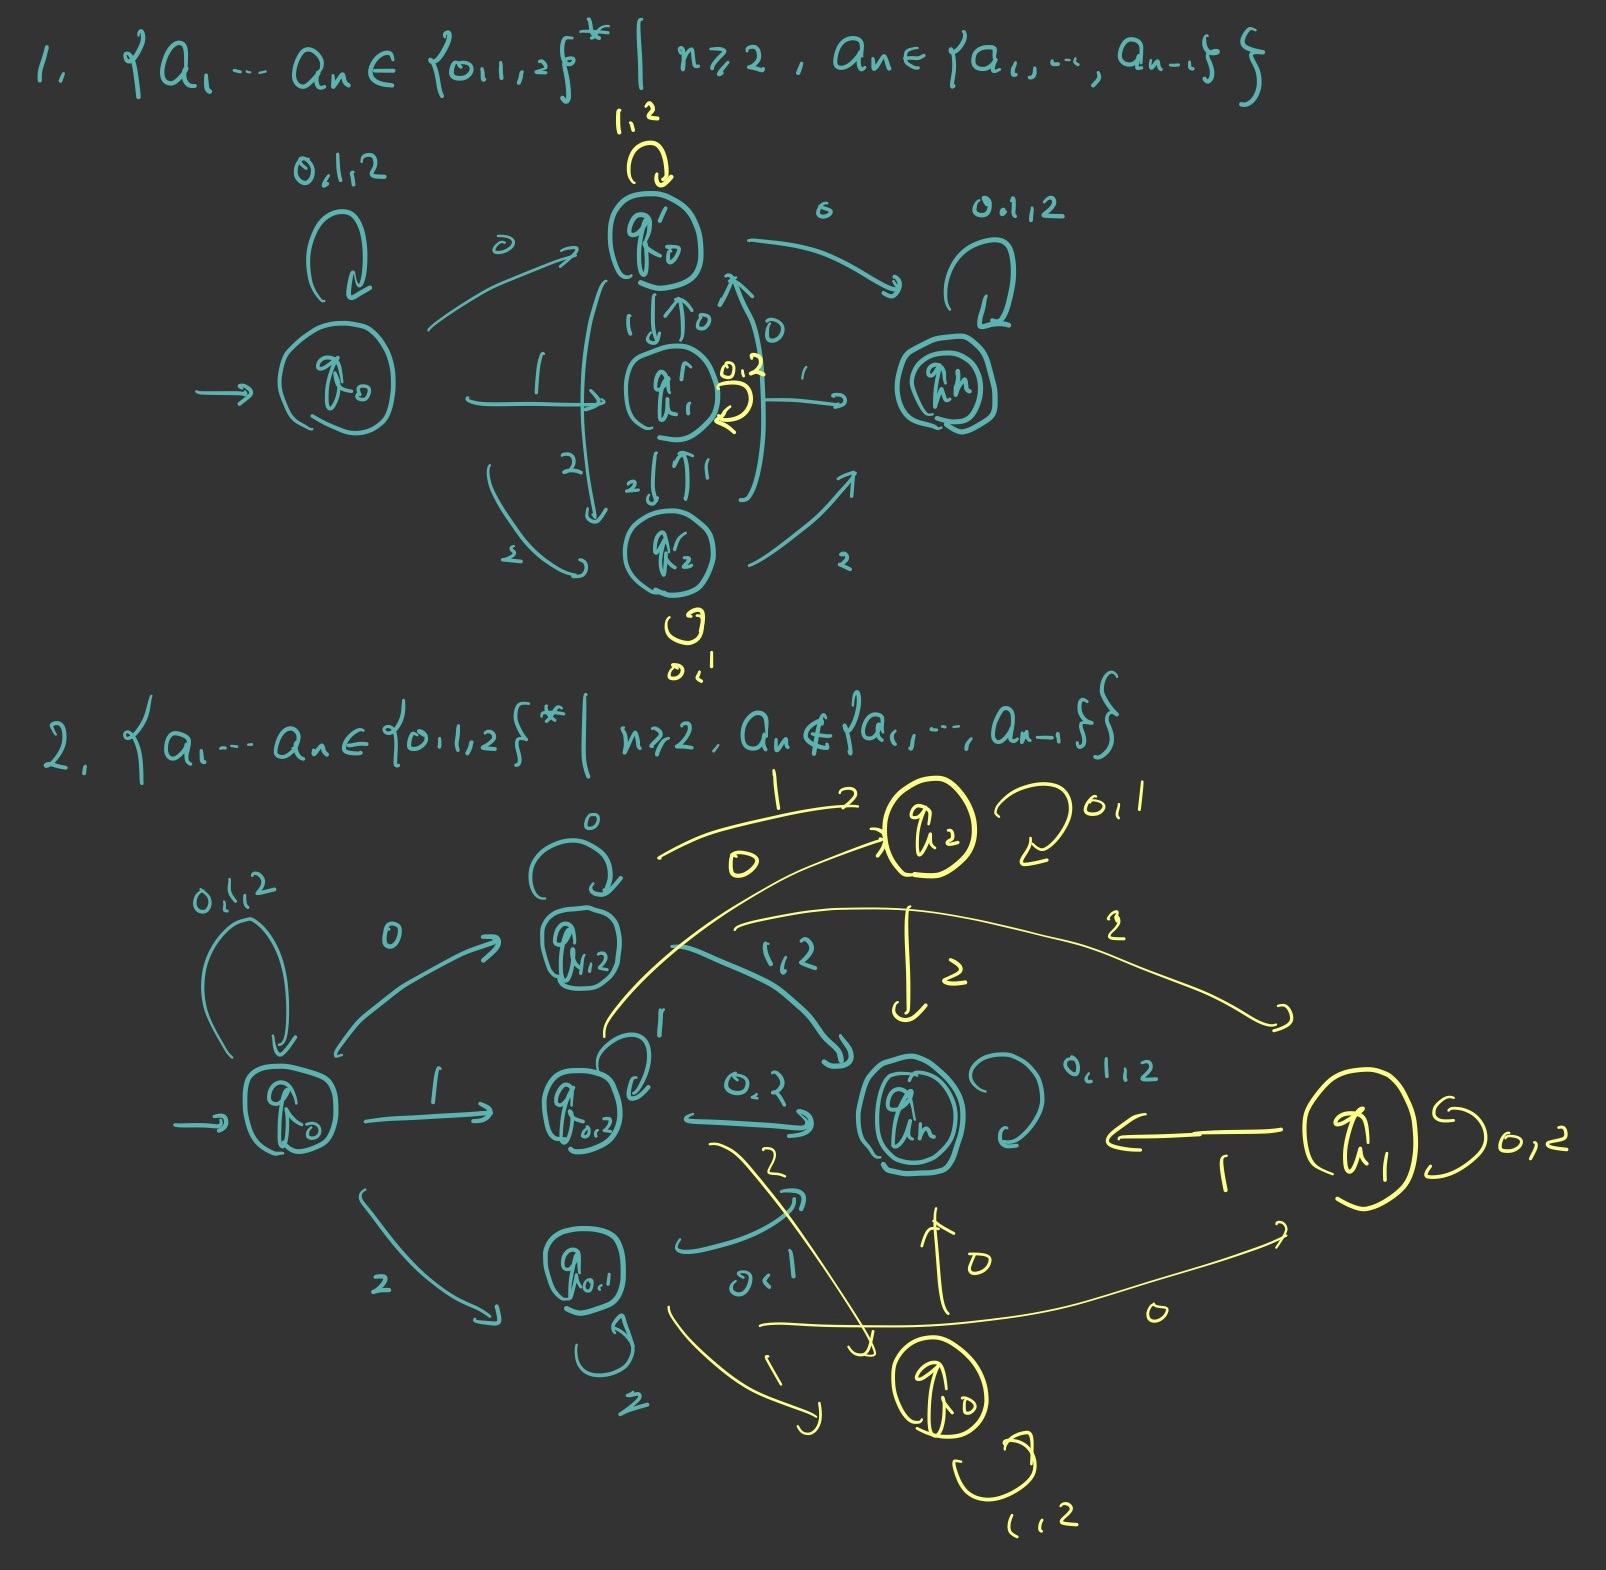
\includegraphics[width=10cm]{automata-1.jpg}
    \end{figure}
\end{example}

「受理計算」の概念を一般化し,任意の2状態間に「到達可能」の概念を定める.

\begin{definition}[accessible]
    2つの状態$p,p'\in M$について,$p$から$p'$に\textbf{到達可能}であるとは,
    記号列$x=a_0\cdots a_n$と,それが定める遷移系列$p\xrightarrow{a_0}p_1\xrightarrow{a_1}\cdots\xrightarrow{a_n}p'$が存在することをいう.
\end{definition}

\begin{proposition}[有限オートマトンの標準形:初期状態から生成される部分について整形(これはオートマトンの同型について同値類をとっているのか?)]
    $M$に対して,次のように定めるオートマトン$M'$について,$L(M)=L(M')$.
    また,$M$が決定的ならば$M'$も決定的である.
    \begin{enumerate}
        \item 初期状態$p_0$から到達可能でない状態を取り除く.
        \item それらを端点とする遷移を取り除く.
    \end{enumerate}
\end{proposition}

\subsection{非決定性オートマトンの応用}

\begin{application}[egrep, fgrep]
    非決定性オートマトンはテキスト検索にも使われる.
    UNIXコマンドegrep, fgrepでは,次の2つを混ぜて実装されている.
    \begin{enumerate}
        \item NFAを模倣するプログラムを書く.
        \item subset constructionでDFAに還元し,それを模倣するプログラムを書く.
    \end{enumerate}
    このクラスの問題に対するsubset constructionでは,状態数の増加が伴わないことが証明できる.
\end{application}

\section{正則言語:決定性に依らない安定な構造}

\begin{screen}
    Autには同型が取れて,有限オートマトンにおいて決定性/非決定性の別は
    それが定める受理言語の観点からは対称であることが分かる.
    なぜなら,その間にはsubset constructionという還元算譜が存在するのである.(まるで座標変換).
    形式言語の圏の中に有限オートマトンが定める言語を,正則言語という.
    これは形式言語のクラスの中で,一番小さい部類のクラスとなる.
\end{screen}

正則言語を定義する前に,Autの中に最後の同型をとっておく必要がある.
一つの非決定性/決定性有限オートマトンに対して,受理言語を共有する
決定性/非決定性有限オートマトンが作れる.

\begin{theorem}[非決定性有限オートマトンと決定性有限オートマトンの等価性]
    言語$L\in P(\Sigma^*)$に対して,次の2条件は同値.
    \begin{enumerate}
        \item $L$は非決定性有限オートンマトンによって受理される.
        \item $L$は決定性有限オートマトンによって受理される.
    \end{enumerate}
\end{theorem}
\begin{proof}
    定義より決定性オートマトンは非決定性オートマトンの特殊な場合としたから
    ($\delta:Q\times\Sigma\to Q$は三項関係の特別な場合に他ならない,あるいは初期状態に余分な自己遷移を加えることによっても),2.$\Rightarrow$1.は成り立つから,$\Leftarrow$を示す.

    非決定性オートマトン$M=(Q,\Sigma,\delta,q_0,F)$から
    次のように構成した(subset construction)決定性オートマトン$\tilde{M}=(\tilde{Q},\Sigma,\tilde{\delta},\tilde{q}_0,\tilde{F})$
    は,同じ言語を受理する:$L(M)=L(\tilde{M})$と示す.
    \begin{enumerate}
        \item $\tilde{Q}:=P(Q)$.
        \item $\tilde{q}_0:=\{q_0\}$.
        \item $\tilde{F}:=\{S\in P(Q)\mid S\cap F\ne\emptyset\}$.
        \item \[\xymatrix@R-2pc{
            \tilde{Q}\times\Sigma\ar[r]^-{\tilde{delta}}&\tilde{Q}\\
            \rotatebox[origin=c]{90}{$\in$}&\rotatebox[origin=c]{90}{$\in$}\\
            (S,a)\ar@{|->}[r]&\{q\in Q\mid\exists p\in S,\;(p,a,q)\in\delta\}
        }\]
    \end{enumerate}
    まず,$L(M)\subset L(\tilde{M})$を示す.
    任意に$w=a_1\cdots a_n\in L(M)$を取ると,$Q$上の受理計算
    \[ q_0\xrightarrow{a_1}q_1\xrightarrow{a_2}\cdots\xrightarrow{a_n}q_n \]
    が存在する.すると,$S_0=\{q_0\},S_i=\{\tilde{delta}(s_{i-1},a_i)\}$とした系列を考えると,構成法より$q_n\in S_n$であるから,$S_n\in F_n$であり,受理計算が構成できたことになる.
    よって,$w\in L(\tilde{M})$である.

    次に,$L(M)\supset L(\tilde{M})$を示す.
    全く同様に,$w\in L(\tilde{M})$の受理計算
    \[S'_0\xrightarrow{a_1}S'_1\xrightarrow{a_2}\cdots\xrightarrow{a_n}S'_n\]
    が$\tilde{M}$に存在する時,
    $q_n\in S'_n$から逆算して,$q_0$からの$M$の系列が作れる.

    よって,上の構成によって,決定性オートマトン$\tilde{M}$について$L(M)=L(\tilde{M})$.
\end{proof}
\begin{remark}
    非決定性オートマトンの余代数を,冪集合構成によって無理やりまとめているのが$\tilde{\delta}$である!
\end{remark}

\begin{definition}[regular set / language]
    (決定性)オートマトンによって受理される集合を\textbf{正則集合}または\textbf{正則言語}という.
    即ち,関手(?)$L:\Aut\to P(\Sigma^*)$の値域である.この集合の族を$\mathcal{R}\subset P(\Sigma^*)$とする.
\end{definition}

\subsection{包含階層}

\begin{definition}[Hierarchy]
    \textbf{包含階層}とは、その要素である集合がその階層の下方にあるすべての集合の真母集合(つまり「集合1⊃集合2⊃集合3⊃...」)になっている構造である。形式言語の階層を構成する言語クラスはそれぞれ言語の集合であり、階層の上方にある言語クラスが下方にあるクラスの言語をすべて含むのがその包含階層である。これらの形式言語は形式文法やオートマトン、モデル理論等によって定義づけられ、大抵の場合その数学的な研究によって階層の中での位置付けを証明される。
\end{definition}
\begin{example}[Chomsky Hierarchy]
    チョムスキー階層は、生成規則による終端および非終端記号からなる文字列の書き換えで定義される、生成文法と呼ばれる形式文法のクラスを軸に定義されている。具体的には、
    \begin{enumerate}\setcounter{enumi}{-1}
        \item [\textbf{帰納的可算言語・部分決定性言語・チューリング受理性言語}]文字列のいかなる書き換えも許される制限なし文法がタイプ-0(これを決定性のある、つまりチューリングマシンが常に停止する言語に限定したクラスが帰納言語で、決定性言語またはチューリング決定性言語とも呼ばれる。)これらの計算複雑性はそれぞれ複雑性クラスRとREに対応する。つまり、与えられた文字列が、その言語の文字列である事を確かめるアルゴリズムを書ける言語の集合が帰納的可算言語で、その言語の文字列で無い事も確かめるアルゴリズムが存在する言語の集合が帰納言語である。
        \item [\textbf{文脈依存言語}]それぞれの生成規則が非終端記号ひとつのみを書き換える文脈依存文法がタイプ-1(文脈自由言語により近い所には、自然言語の研究から弱文脈依存言語というクラスが設定されている。)
        \item [\textbf{文脈自由言語}]文脈依存文法のうち前後の文字列に依存せず書き換える文脈自由文法がタイプ-2
        \item [\textbf{正規言語}]文脈自由文法のうち書き換えが終端記号一つまたは終端および非終端記号一つずつである正規文法がタイプ-3.有限オートマトンが定める.
    \end{enumerate}
    下方の文法クラスがそれぞれ上方の文法クラスすべての真部分集合となっているため、対応する言語も包含階層が成立する。なお、それぞれに対応するオートマトンもよく知られている。
\end{example}

\section{$\epsilon$動作付き非決定性有限オートマトン}

\begin{screen}
    非決定性オートマトンを拡張する.
    $\epsilon$動作付き非決定性有限オートマトンはさらに人間がプログラムし易い高級言語となっている.
    $\epsilon$遷移の除去算譜が存在するために,これが定め得る言語も,正則言語に一致する.
\end{screen}

\begin{definition}[$\epsilon$-transition, $\epsilon$-NFA]
    空語$\epsilon$を読んで行う遷移を\textbf{$\epsilon$-遷移}という.

    非決定性オートマトンの状態遷移関係$\delta\subset Q\times\Sigma\times Q$を,$\delta\subset Q\times(\Sigma\cup\{\epsilon\})\times Q$としたものを,
    \textbf{$\epsilon$-動作付き非決定性有限オートマトン}という.
\end{definition}

\begin{definition}[$\epsilon$-closure]
    $\epsilon$-閉包ECLOSE$(q)\subset Q$を次のように機能的に定義する.
    \begin{enumerate}
        \item $q\in\mathrm{ECLOSE}(q)$.
        \item $p_1\in\mathrm{ECLOSE}(q)$とする.$\exists a\in\Sigma, (q_1,a,q_2)\in\delta$(または$q_2\in\delta(p_1)$)ならば,$q_2\in\mathrm{ECLOSE}(q)$.
    \end{enumerate}
\end{definition}

\begin{definition}[遷移関数の拡張と,$\epsilon$動作付き非決定性有限オートマトンが定める言語]
    $\delta^*:Q\times(\Sigma\cup\{\epsilon\})^*\times Q$を次のように帰納的に定義する.
    \begin{enumerate}
        \item $\delta^*(q,\epsilon)=\mathrm{ECLOSE}(q)$.
        \item 
    \end{enumerate}
\end{definition}

\begin{theorem}[等価原理と$\epsilon$遷移の除去算譜]
    言語$L\in P(\Sigma^*)$に対して,次の2条件は同値.
    \begin{enumerate}
        \item $L$は$\epsilon$動作付き非決定性有限オートンマトンによって受理される.
        \item $L$は決定性有限オートマトンによって受理される.
    \end{enumerate}
\end{theorem}


\begin{proposition}
    任意のinput alphabet $\Sigma$について,任意の有限部分集合$L\subset\Sigma^*$は正則言語である.
\end{proposition}
\begin{proof}
    次のようにして$\epsilon$-動作付き非決定性有限オートマトンを構成すれば良い.

\end{proof}

以上の有限状態機械は,無限にも定義を拡張できる.

\section{正則言語の反復補題}

\begin{screen}
    記号列の無限集合を認識する有限オートマトンは,必ずループを持つ.
    この正則言語(やその他の形式言語のクラス)の必要条件を,反復補題という.
\end{screen}

\begin{theorem}[Pumping Lemma]\label{thm-Pumpimg-lemma}
    $L\subset\Sigma^*$を正則言語とする.
    このとき,ある定数$N\ge 1$が存在して,長さが$N$以上の記号列$x\in L\land |x|\ge N$ならば,
    その分解$x=uvw$であって,
    \begin{enumerate}
        \item $1\le |v|<N$(これよりも粗い条件である$1\le |v|\land 1\le|uv|\le N$としても示せる),
        \item $\forall m\in\N,\; uv^mw\in L$,
    \end{enumerate}
    の2条件を満たすものが存在する.
\end{theorem}
\begin{proof}
    $L$は正則言語であるから,これが定める決定性有限オートマトンを$M=(Q,\Sigma,\delta,q_0,F)$とする.
    $N=|Q|$とすれば,$\{q_0\}\subset Q$より$N\ge 1$を満たす.
    $|x|=:n\ge N$を満たす$x\in L$を任意に取る.すると$x$が定める受理計算が存在するが,その系列の長さは$|Q|$を超えているから,
    鳩の巣原理より同じ状態が少なくとも2回現れる:$\exists i,j\in n+1,\;(0<)j-i\le N\land p_i=p_j$.
    これについて,
\end{proof}
\begin{remark}
    Y. Bar-Hillel, M. Perles, E. Shamir, "On formal properties of simple phrase structure grammars", Zeitschrift für Phonetik, Sprachweissenshaft und Kommunikationsforschung 14 (1961) pp. 143-172.

    反復補題(英: Pumping lemma)とは、計算可能性理論において、あるクラスの形式言語に反復を施してもそのクラスに依然として属することを示すものである。ここでいう「反復」とは、その言語に含まれる十分に長い文字列が部分に分割可能で、その一部分を繰り返したさらに長い文字列も同じ言語に含まれるようにすることである。この補題の証明には、鳩の巣原理のような組合せ数学が必要とされる。
    反復補題の重要な具体例として、正規言語の反復補題と文脈自由言語の反復補題がある。文脈自由言語の反復補題の一種として、オグデンの補題もある。
    これらの補題は、ある言語が特定の言語クラスに属さないことを示すのに使われる。しかし逆に、反復補題を満たすことは必要条件ではあっても十分条件ではないので、ある言語があるクラスに属することを示すのには使えない。
\end{remark}

\begin{corollary}
    言語$L=\{0^n1^n\mid n\in\N\}$は正則ではない.
\end{corollary}
\begin{proof}
    $L$を正則とする.
\end{proof}

\begin{corollary}[回文]
    言語$L=\{ww^R\mid w\in\{0,1\}^*\}$は正則ではない.
\end{corollary}
\begin{proof}
    $L$を正則とする.
\end{proof}

\section{正則表現}

\begin{screen}
    正則言語と有限オートマトンの等価性を得た.
    ここで,正則言語に対する代数的記法を1つ導入する.
    これは実用化されているほど強力な代数的手法で,生成の概念を捉えている1つの形式言語である.
\end{screen}

\begin{definition}[regular expression / regex]
    \textbf{アルファベット$\Sigma$上の正則表現}とは,アルファベット$\Sigma\cup\{*,+,),(,\emptyset\}$上の記号列$\REGEX\subset P(\Sigma\cup\{*,+,),(,\emptyset\})$であって,次のように帰納的に定義されるものである.
    解釈写像$L:\REGEX\to P(\Sigma^*)$が定まる.言語$L(r)\subset\Sigma^*$と正則表現$r$を混同することも多い.
    \begin{enumerate}
        \item 空列を表す記号$\emptyset$は正則表現である:$L(\emptyset)=\emptyset$.
        \item 各アルファベット$a\in\Sigma$は正則表現である.語$a$を表す:$L(a)=\{a\}$.
        \item $r,s$を正則表現とすると,$(r+s),(rs),(rs^*)$は正則表現である:$L(r+s)=L(r)\cup L(s), L(rs)=L(r)L(s),L(r^*)=L(r)^*$.
        \item 以上のように定義されるもののみが正則表現である.
    \end{enumerate}
\end{definition}
\begin{example}\mbox{}
    \begin{enumerate}
        \item $L((0+1)^*)=\{0,1\}^*$.
        \item $(0+1)^*00(0+1)^*$は2つ以上続く$0$を持つ文字列全体の集合を表す.
    \end{enumerate}
\end{example}

\begin{lemma}[代数的構造:集合代数から輸入]
    次の正則表現上の等式は,解釈写像$L$とSetをモデルとして充たされる.
    (即ち,正則表現上の$=$は解釈写像$L$を用いて集合の相等として解釈する).
    \begin{enumerate}
        \item $r+s=s+r$.和集合の可換性$L(r)\cup L(s)=L(s)\cup L(r)$より.
        \item $(r+s)+t=r+(s+t)$.和集合演算の結合性から.
        \item $(rs)t=r(st)$.
    \end{enumerate}
\end{lemma}

\chapter{文脈自由文法とプッシュダウンオートマトンの理論}


\part{集合論}

\chapter{ZFCとvon Neumann hierarchy}

Russellの逆理は,素朴な意味での「ものの集まり」と言った言及を再帰的に許すことによって生じる.
従って,「ものの集まり」に階層付けすることが一つの対応となる.ここではZFC公理系を考える.
公理から集合を定義し,そこから数や関数や基数の定義を引き出して,確かに数学全体の基礎を与える方法の1つであることを確認し,
同時にZFC内外での集合やクラスの更なる取り扱いを議論する.

\section{準備}

\begin{definition}[axiom schema]
    論理式全体$Fml_L$を走る変数を伴った2階の論理式が存在して,その変数に論理式を代入した結果だと捉えられる,論理式の集合のことを\textbf{公理図式}という.
\end{definition}
\begin{example}
    推論規則は公理図式である.
\end{example}

\begin{shadebox}
    \begin{definition}[集合の公理系ZF]\label{def-ZF-theory}集合の公理は,集合論の言語$L=\{=,\in\}$による一階述語論理の言葉で,次のように表せる.ただし,自由変項から始まる公理は,全称量子化(universally quantified)されているものとする.
        \begin{enumerate}\setcounter{enumi}{-1}
            \item (Set Existence). $\exists x(x=x)$
            \item (Extentionality). $\forall z(z\in x\leftrightarrow z\in y)\rightarrow x=y$
            \item (Foundation). $\exists y(y\in x)\rightarrow\exists y(y\in x\land \lnot\exists z(z\in x\land z\in y))$
            \item (Comprehension Scheme). 自由変項$y$を持たないような全ての式$\varphi$について,
            \[\exists y\forall x\;(x\in y\leftrightarrow x\in z\land\varphi(x))\]
            \item (Pairing). $\exists z(x\in z\land y\in z)$
            \item (Union). $\exists A\forall Y\forall x(x\in Y\land Y\in\mathcal{F}\rightarrow x\in A)$
            \item (Replacement Scheme). 自由変項$B$を持たないような全ての式$\varphi$について,
            \[\forall x\in A\exists!y\varphi(x,y)\rightarrow\exists B\forall x\in A\exists y\in B\varphi(x,y)\]
        \end{enumerate}
        以降,一階述語論理の文字列に対して,次の略記となるような述語を採用する.
        \begin{screen}
            \begin{notation}\mbox{}
                \begin{enumerate}[(i)]
                    \item $x\subset y:\Leftrightarrow\forall z(z\in x\rightarrow z\in y)$
                    \item $x=\emptyset:\Leftrightarrow\forall z(z\notin x)$
                    \item (Ordinal successor function). $y=S(x):\Leftrightarrow\forall z(z\in y\leftrightarrow z\in x\lor z=x)$
                    \item $w=x\cap y:\Leftrightarrow\forall z(z\in w\leftrightarrow z\in x\land z\in y)$
                    \item (isSingleton). $\mathrm{SING}(x):\Leftrightarrow\exists y\in x\forall z\in x(z=y)$
                \end{enumerate}
            \end{notation}
        \end{screen}
        \begin{enumerate}\setcounter{enumi}{6}
            \item (Infinity). $\exists x(\emptyset\in x\land \forall y\in x(S(y)\in x))$
            \item (Power Set). $\exists y\forall z(z\subset x\rightarrow z\in y)$
            \item (Choice). $\emptyset\in F\land\forall x\in F\forall y\in F(x\ne y\rightarrow x\cap y=\emptyset)\rightarrow \exists C\forall x\in F(\mathrm{SING}(C\cap x))$
        \end{enumerate}
    \end{definition}
\end{shadebox}
\begin{remark}\mbox{}
    \begin{enumerate}
        \item このZermelo-Fraenkel styleでは,宇宙は,全ての遺伝的集合のクラスとなる.
        特に7.無限公理の採用の仕方が,順序数を念頭においている.これが特徴的で最初は慣れなかった.
        2.整礎性公理は,全ての集合$x$について,順序数$\alpha$が存在して$x\in V_\alpha$であることに同値である.
        \item 1~9をZFC, 1~9をZF,これらから6.置換公理を除いたものをそれぞれZC, Zといい,
        これら4つからそれぞれ2.整礎性公理を除いたものを$\mathrm{Z^-,ZF^-,ZC^-,ZFC^-}$という.
    \end{enumerate} 
\end{remark}

集合はその元によって決まる.この大前提を外延性公理という.外延と内包という二項対立の中の,一方の極にポジションを取った.

\section{集合生成規則}

\subsection{集合全体のクラス$V$}

\section{順序,整礎関係,超限帰納法}

\section{整列順序と順序数}

\subsection{整列順序}

\subsection{順序数}

\begin{definition}
    集合$x$のランクとは,$x\in V_\alpha$を満たす最小の順序数$\alpha$である.
\end{definition}

\subsection{順序数演算}

\subsection{木}

\section{濃度と基数}

\subsection{基数演算}

\subsection{帰納的定義入門}

\section{フィルターと閉非有界集合}

\subsection{集合上のフィルター}

\subsection{ブール代数}

\subsection{閉非有界集合}

\subsection{posetとMartinの公理MA}

\section{Ramseyの定理}

\section{遺伝的有限集合}

遺伝的有限集合とは,有限個の遺伝的有限集合からなる集合のことを指す.遺伝的有限集合全体のクラス$V_\omega$は,ランク$\omega$の累積的階層であり,従って遺伝的整礎集合全体のクラスの部分クラスである.
また,ZF公理系の7.無限公理をその否定で置き換えた公理系のモデルをなす.即ち,無限公理は,他の公理から独立である.各$V_n$の濃度は${}^{n-1}2$であるから,遺伝的有限集合は全部で可算無限個存在する.
同型の例として,Ackermannの符号化が構成できる.

\begin{definition}[遺伝的有限集合 hereditarily finite set]
    遺伝的有限集合を,次のように帰納的に定義する.

    1. 空集合は遺伝的に有限である.

    2. 遺伝的に有限な集合$a_1,\cdots,a_n$について,集合$\{a_1,\cdots,a_n\}$は遺伝的に有限である.

    3. 以上によって遺伝的に有限だとわかる集合のみが遺伝的有限集合である.
\end{definition}
\begin{remark}
    実は「遺伝的」の部分は,Material Set Theoryによる構成の仕方を指定しているだけで,結局はただの有限集合である.しかし,「有限集合全体の集合」は一般に集合とは言えないが,「遺伝的有限集合全体の集合」は構成方法までよく定まっていて,確かに可算な集合である.
    As a property of a set, being hereditarily finite is equivalent (up to isomorphism of sets) to simply being finite. So the ‘hereditary’ part is meaningful only in material set theory, not structurally, unless you see it as a property of a pure set represented structurally as a membership tree.\footnote{nLab}
\end{remark}

\begin{proposition}
    1. 集合は遺伝的に有限である.

    2. 集合の推移的閉包は有限集合である.
\end{proposition}

\begin{proposition}[遺伝的有限集合全体のクラス]
    集合$V_n$を次のように定める.

    1. $V_0=\varnothing$

    2. $V_{n+1}=P(V_n)$

    最後に,$V_\omega=\bigcup_{n<\omega}V_n$とすれば,これは遺伝的有限集合全体のクラスである.
\end{proposition}
\begin{remark} 

    1. これは,von Neumann宇宙(遺伝的整礎集合全体のクラス)の部分クラスになる.

    2. $V_{\omega+\omega}$はordinary mathematicsの宇宙であり,Zermeloの公理系のモデルである.

    3. $V_\kappa$はZFC集合論のモデルである.

    これは,ZF公理系において,無限公理をその否定と置き換えたもののモデルになる.即ち,無限公理は他のZFの公理からは独立であることがわかる.
\end{remark}

\begin{proposition}[Ackermann (1937)]
    遺伝的有限集合全体のクラス$V_\omega$について,$V_\omega\simeq\omega$である.
\end{proposition}
\begin{proof}
    Ackermannの符号化$f:\mathbb{N}\to V_\omega$を,遺伝的集合の階数に関する帰納法によって,
\end{proof}

\part{証明論}

\chapter*{証明論とは}

証明論とは,証明という行為について数学的な解析を行う数理論理学の分野である.
より一般的に,推論や思弁について考える哲学の論理学の一分野とも言える.

次がwikipediaの「形式的証明と非形式的証明」の欄であるが,この形式と非形式,形式という
言語機能を高度に抽象化させたものと非形式と自然言語との対応について考えたい.
どうして言語機能の先に,計算能力を持ったのか.
\begin{quotation}
    数学で日常的に行われている「非形式的」証明は、証明論で言う「形式的」証明とは異なる。しかしながら、それは形式的証明の高度に抽象化されたスケッチのようなもので、専門家が十分な時間と忍耐を持っていれば、非形式的証明から形式的証明を適切に再構築できるようなものである場合が多い。比喩的に言えば、そのような場合に完全な形式的証明を書くことは、機械語でプログラミングをするようなものである。

    現代では、形式的証明は一般に計算機支援証明を補助としてコンピュータを使って構築される。また、その証明がコンピュータで自動的に検証される点も重要である。形式的証明の検証は簡単だが、証明そのものをコンピュータが構築すること(自動定理証明)は一般には非常に困難である。一方、数学における非形式的証明は査読による検証に何週間も要し、それでもまだ誤りが含まれていることが多い。
\end{quotation}

\chapter{様々な証明体系}

\begin{definition}[形式論理/記号論理]
    数学や哲学に於ける論証(argument)という営みを抽象化した「モデル」
    または「形式言語」を,\textbf{形式論理・記号論理}という.このモデル化のことを\textbf{形式化}という.
\end{definition}
\begin{remark}
    形式化は,現代数学の基本的な戦略であると同時に,計算機が扱える対象への変換をも意味する.
    従って,形式論理における推論を計算機を用いて自動化することも可能である.
\end{remark}

\section{形式論理前史}
証明論の始祖はGentzenであると言えるが,その前の大事な母胎はAlfred WhiteheadやBertrand Russell,またFregeとHilbertが作った.
当時から論理計算が存在した.
\begin{quote}
    公理的命題論理のバージョンによって採用する公理や推論規則が異なる。例えば、フレーゲは、6つの公理と2つの規則を採用した。バートランド・ラッセルとアルフレッド・ノース・ホワイトヘッドは、5つの公理からなる体系を示唆した。\footnote{ja.wikipedia.org「自然演繹」}
\end{quote}

\section{自然演繹(natürlichen Schließens)}
\begin{quote}
    このG. Gentzenの学位論文(G. Gentzen, Untersuchungen über das logische Schließen, Math. Zeitschr. 39(1934/35), I, 176-210: II, 405-431.)こそが証明論という分野をいまあるかたちにあらしめたものである.\cite{新井敏康-Gentzen}
\end{quote}
自然演繹は,論証はいくつかの定まった推論(inference)から構成され,その構成子の種類によって論証の性質が定まる,という非常に直観的なモデル設計である.
換言すれば,論証を推論の繰り返し,簡約の繰り返し,従って計算と見てる計算モデルである.
実際,自然演繹の体系は型付ラムダ計算と同一視出来る.これを\textbf{論理計算(logical calculus)}という.
\begin{quote}
    論理計算はFrege, Russell, Hilbert以来,既にあり,その完全性もK. Gödelによって示されていたのだが,新たにこれらの論理計算を導入した理由をGentzenは「実際の推論にできる限り近い形の形式的な論理体系を作る」ためであったと書いている.
    さらにGentzenは NJ, NKが「或る独特な性質(正規化定理のこと)をもっているということや,さらにその点に関しては,直観主義者が否認するところの‘排中律’が特殊な地位を占めているということもわかってきた」と続ける.
    導入則と除去則がセットになった9つの推論規則があり,これらはBHK解釈(Brouwer-Heyting-Kolmogorov interpretation)に似て,いわばそれぞれの論理結合詞の(操作主義的)意味を規定する.\cite{新井敏康-Gentzen}
\end{quote}

学位論文で提出されたのは2つのモデル,NKとNJである.

\subsection{推論規則}
自然演繹では,証明を\textbf{証明図(proof figure)}または\textbf{証明木(proof tree)}として実装する.

\begin{definition}[proof figure / proof tree]
    \textbf{証明図}とは,「仮定」と呼ばれる0個以上の論理式$A$と「結論」と呼ばれる1個以上の論理式$C$とを持ち,\textbf{推論規則}に対応する長い横棒の3組$(A,B,I)$である.
    これを$\frac{A}{C}I$とも書く.
    \textbf{証明木}とは,論理式を節点とし推論規則を枝とする木である.
\end{definition}
\begin{remark}
    証明図は射である.例えば,$A$を論理式として,$A=\{A\},C=\{A\},I=\varnothing$という単位射も証明図である.
    というより,退化した証明図を命題という.また,前件が空な証明図を定理という.

    また,合成について閉じている.
\end{remark}

\begin{notation}[証明図]
    $\Pi,\Delta$などで証明図を表す.
    \begin{center}
        \begin{tikzcd}
            B_1B_2\cdots B_n \ar[d, dotted, no head, "\Pi"] \\
            A
        \end{tikzcd}
    \end{center}
    で仮定を$B_1,\cdots,B_n$(この集合を$\{B_1,\cdots,B_n\}=:\Gamma$と置くことも多い),結論を$A$とする証明図$\Pi$を表す.
    ただし,仮定はいくつか省略し,大事なものだけを書くことも多い.
\end{notation}
\begin{notation}[ならば]
    ならばの記号はSequent計算にて衝突が起こるので,$\supset$を使う.
\end{notation}

\begin{definition}[証明図の構成(合成)]
    証明図の構成は次の様に行う.2つの図式
        \begin{center}
            \begin{tikzcd}
                \Gamma \ar[d, dotted, no head, "\Pi_1"] & & \Gamma \ar[d, dotted, no head, "\Pi_2"] \\
                A & & B
            \end{tikzcd}
        \end{center}
        があったとする.この時,次の証明図を構成できる.この時の\textbf{長い横棒を推論規則と呼び,推論規則を公理により定める}ことで自然演繹の体系が作られる.
        \begin{center}
            \begin{tikzcd}
                & \Gamma \ar[d, dotted, no head, "\Pi_1"] & \Gamma \ar[d, dotted, no head, "\Pi_2"] & \\
                & A & B & \\
                {} \ar[rrr, no head] & & & \land I\\
                & {} \ar[r, phantom, "{A\land B}"] & {} &
            \end{tikzcd}
        \end{center}
        この証明図の仮定は,特に解除もされていないので$\Gamma$のままである.
        証明図が構成されるにあたって,仮定が変化すること(のうち特に仮定が外れること)を脱落(close, discharge)といい,
        dischargeされる仮定に記号[ ]を付けて,またdischargeされる構成に所属する横棒の隣に推論規則の名前
        にdischargeに対応する添字を添えて表現される.
    
        以上の証明図の構成を,よく新たに作られた証明図のみを書き,証明図の構成法である推論規則の表現とする.
\end{definition}

従って,証明の構成/論証の構成は,命題$A$からなる自明な証明図から開始して,
証明図の構成の連鎖として理解される.

\begin{definition}[weakening]
    証明図内に新たな仮定を加える構成を\textbf{水増し}という.
\end{definition}

\begin{definition}[証明可能性]
    規定された推論規則により導出可能であることを,\textbf{NJ,NKにて証明可能}といい,それぞれ$\vdash_{NJ},\;\vdash_{NK}$と表す.
    図式記号の$\Pi$や$\Gamma$や$\Phi,\Psi$と同様,メタ言語の記号である.
\end{definition}
\begin{remark}
    述語$\vDash$はモデル論のものか?
\end{remark}

\begin{screen}
    証明図は書いてみた感じ,普段の証明の形式化そのものである.statementを見れば,「仮定して矛盾を示せば良いな」.
    「これは仮定して矛盾を示す方針しかあり得ないが,二重否定則がないと帰ってこれないので,NKの範囲でしか成り立たないな」とわかる(特定の方向のDe Morgan則など).
    NJ,NKはそれぞれ自然な閉包だと感じられるが,なんの閉包なのかあまりわかっていない.
\end{screen}

\subsection{NJ:直観主義論理}
この範囲で型付きラムダ計算との対応を持つ.

\begin{definition}[NJ]
    推論体系NJは次の9つの推論規則(証明図から次の証明図を得る際に許された操作)からなる.
    4つの論理式についての導入則(I)と除去則(E)と$\bot$の扱いについての特徴付け1つからなる.
    \begin{enumerate}
        \item $\frac{\Phi\;\;\;\;\Psi}{\Phi\land\Psi}\land I$
        \item $\frac{\Phi\land\Psi}{\Phi}\land E_L,\;\frac{\Phi\land\Psi}{\Phi}\land E_R$
        \item   $[A]$\\
          $\vdots$\\
        $\frac{\Psi}{\Phi\supset\Psi}\supset I$
        \item $\frac{\Phi\;\;\;\;\Phi\supset\Psi}{\Psi}\supset E$
        \item $\frac{\Phi}{\Phi\lor\Psi}\lor I_L,\;\frac{\Psi}{\Phi\lor\Psi}\lor I_R$
        \item      $[A]^l\;\;[B]^l$\\
             $\vdots$ $\vdots$\\
        $\frac{\Phi\lor\Psi\;\;\;\;X\;\;\;\;X}{X}\lor E;l$
        \item  $[\Phi]^l$\\
        $\vdots$\\
        $\frac{\bot}{\lnot\Phi}\lnot I;l$
        \item $\frac{\Phi\;\;\;\;\lnot\Phi}{\bot}\lnot E$($\bot I$とも見れる)
        \item $\frac{\bot}{A}\;\bot$
    \end{enumerate}
    仮定$\Gamma$の省略の流儀に沿った.
\end{definition}

NJでは矛盾に関する規則は次が使われる.
\begin{definition}[absurdity rule]
    次の推論規則を\textbf{不条理則・$\bot$除去則}という.
    \[ \frac{\bot}{A}\;\bot \]
\end{definition}

\begin{proposition}[ARよりも弱い命題なら常に成り立つ]
    \[\forall\phi,\;\bot\vdash_{NJ,NK}\lnot\phi\]
\end{proposition}
\begin{proof}$bot,[\phi]^l$について,
    1.$\land I$,2.$\land E$,7.$\lnot I$から導ける.
\end{proof}
\begin{remark}
    どうやら\cite{論理と計算のしくみ}はこれがabsurdity ruleと同値という立場なのかな?
\end{remark}

\begin{proposition}[ARの妥当性]
    次のWorkspaceを,選言三段論法(Disjunctive syllogism / modus tollendo ponens)という.
    \[\frac{\Phi\lor\Psi\;\;\;\;\lnot\Phi}{\Psi}DS\]
    次の2条件は,NJ上同値である.
    \begin{enumerate}
        \item 不条理則$\bot E$が成り立つ.
        \item $\lor I$かつ選言三段論法が成り立つ.
    \end{enumerate}
\end{proposition}
\begin{proof}
    まず1.$\Rightarrow$2.は,場合分けにより,不条理則のみを使ってDSを示せる.

       $[\Phi]^l\;\lnot\Phi$\\
        $\vdots\;\bot I$\\
    $\frac{\Phi\lor\Psi\;\;\;\;\Psi\;\;\;\;[\Psi]^l}{\Psi}\lor E;l$
    
    次に,2.$\Rightarrow$1.は,$\bot\cdots_{\lor I}\bot\lor\Psi$と$[\bot]^l\cdots_{\lnot I}\lnot\bot$から,DS;lにより$\Psi$を得ることが出来る:$\bot\vdash_{NJ,NK}\Psi$.
\end{proof}

\subsection{NK:古典論理}

NJで不条理則に当たるものは,次の背理法で置換される.
\begin{definition}[reductio ad absurdum]
    \textbf{背理法・帰謬法・不条理則}は次の証明図に表される推論規則をいう.普通仮定は省略される.
    \[
        \xymatrix{
            {[\lnot A]^l}\ar@{.}[d]\\{\bot}\ar@{}[d]|{---}&{}\ar@{}[d]^-{RAA;l}
            \\A&{}
        }
    \]
\end{definition}
その結果,全ての命題に2値のいずれかが対応する体系となる.
なお,この(古典的)背理法,二重否定の除去則,Pierceの法則,あるいは排中律$\Phi\lor\lnot\Phi$のどれを9個目として
採用しても等価な体系を得る.

\begin{proposition}[double negation elimination]
    次の推論規則を\textbf{二重否定の除去則}という.
    \[
        \xymatrix{
            {}\ar@{.}[d]&\\{\lnot\lnot A}\ar@{}[d]|{---}&{}\ar@{}[d]^-{\lnot\lnot E}
            \\A&{}
        }
    \]
    次の2条件は,NJ上同値である.
    \begin{enumerate}
        \item 排中律かつ不条理則が成り立つ.
        \item 二重否定則が成り立つ.
    \end{enumerate}
\end{proposition}

\begin{proposition}[二重否定の除去則は不条理則よりも強い]
    \[\bot\vdash_{NK}\Phi\]
\end{proposition}
\begin{proof}
    $\frac{\bot}{\lnot\Psi\supset\bot}$と$[\lnot\Psi]^l$から$\supset E$より$\bot$を得る.$\lnot I;l$より$\lnot\lnot\Psi$を得る.二重否定の除去則より$\Psi$を得る.
\end{proof}
\begin{remark}
    こういうものは$\Phi,\lnot\Phi\vdash_{NK}\Psi$を$\bot$に置き換えることで証明を得る.

    同様に,NJの証明をこれで置き換えると全てNKの証明になる.
\end{remark}

\begin{proposition}[二重否定の除去則]
    二重否定の除去則が成り立つならば,不条理則も成り立つ.
\end{proposition}

\begin{proposition}[Peirce's law]
    次の証明図を\textbf{パースの法則}という.
    \[ \frac{}{((A\supset B)\supset A)\supset A}\;\mathrm{Peirce's\;law} \]
    $\vdash_{NK}\mathrm{Peirce's\;law}$である.
\end{proposition}

\begin{proposition}[the Law of Excluded Middle]
    次の証明図を\textbf{排中律}という.
    \[ \frac{}{\Phi\lor\lnot\Phi}\;\mathrm{EM} \]
    $\vdash_{NK}\mathrm{EM}$である.
\end{proposition}

\subsection{一階への拡張}
この体系に無理やり同型対応を入れたら,どんなラムダ計算が出来上がるのだろう?

\begin{definition}
    直観主義論理,古典論理の別に拘らず,次が一階の言語についての拡張となる.
    \begin{enumerate}
        \item  $\vdots$\\
        $\frac{\forall xA[x]}{A[t]}\forall E$
        \item $\Gamma$\\
        $\vdots$\\
        $\frac{A[y]}{\forall xA[x]}\forall I$(ただしこの時$\Gamma$とは$A[y]$を導くにあたってundischargedな全ての仮定を表している,また$\Gamma$内に$y$の自由な出現はないものとする).「$y$を任意に取る」というやつである.
        \item $\vdots$\\
        $\frac{A[t]}{\exists xA[x]}\exists I$
        \item    $[A[y]]\l\;\;\;\Gamma$\\
             $\vdots$\\
        $\frac{\exists xA[x]\;\;\;\;C}{C}\exists E;l$
    \end{enumerate}
    これに$=$の導入則$\frac{}{t=t}=I$と除去則$\frac{A[t]\;\;\;\;t=s}{A[s]}$を含める流儀もある.
\end{definition}
\begin{remark}
    =Eが「等しい両辺ならくっつけられる」とかではなく,論理式への置換であるところが強力である.多分.
\end{remark}

\subsection{Curry-Howard対応}
W. Howard, The formulae-as-types notion of construction, in J. P. Seldin, J. R. Hindley (eds), To H.B. Curry: Essays on Combinatory Logic, Lambda Calculus and Formalism, Academic Press, 479-490(1982).
で指摘された.
\begin{quote}
    自然演繹での証明とプログラムの対応および命題と型の対応,
    さらに証明の変形と型付きラムダ計算における計算との対応は,
    [Howard82]においてCurry-Howard対応(isomorphism)として定式化されて
    証明論と理論的計算機科学の交流をもたらした,cf. [Girard89].
    さらにPer Martin-Löf, An intuitionistic theory of types, Twenty-five years of constructive type theory, Oxford Logic Guides 36, pp. 127–172, Oxford UP(1998).における型理論はBHK解釈と自然演繹に刺激を受けているものと考えられる.
\end{quote}

\subsection{Glivenkoの定理とGödelの二重否定翻訳}

\begin{theorem}
    $\Gamma$を命題論理式の有限集合,$\Phi$を命題論理式とする.
    次の2条件は同値である.
    \begin{enumerate}
        \item $\Gamma\vdash_{NK}\Phi$
        \item $\Gamma\vdash_{NJ}\lnot\lnot\Phi$
    \end{enumerate}
\end{theorem}
\begin{remark}
    於戯面白い,これは古典論理と直観主義論理との関係についての直観もちょうど芽生えていたものだ.
    この定理はつまり,「古典論理と直観主義論理は,"戻ってこれない"点を除いて違いはない」ことを保証したもので,
    古典論理の証明は,最後に一回だけまとめて二重否定の除去則を使えばいいという証明の標準的な方針を与える.
\end{remark}

しかし,一階論理では次の段階について次の結果が成り立つので,一般にGlivenkoの定理は成り立たない.
\begin{proposition}[クリプキモデル]
    (1)を$\lnot\lnot\forall x\Phi(x)$,(2)を$\forall x\lnot\lnot\Phi(x)$とする.
    次の2条件が成り立つ.
    \begin{enumerate}
        \item $(1)\vdash_{NJ} (2)$が成り立つ.
        \item $(2)\vdash_{NJ} (1)$は成り立たない.
    \end{enumerate}
\end{proposition}

\subsection{正規化定理とシーケント計算}
正規化定理はステートメントも証明もGentzenの学位論文にはなく,
正規化定理の証明の出版にはD. Prawitz, Natural deduction. A proof-theoretical study, Almqvist and Wiksell, 1965.を待たなければならなかった.
なお,Gentzenは A. Turingによる型付きラムダ計算に対する正規化定理と同工異曲の証明を少なくともNJに対しては持っていたことがわかっている.
「この[Prawitz65]は当時の証明論に自然演繹の復権をもたらしたと思う.」とのことである\cite{新井敏康-Gentzen}.
\begin{quote}
    Gentze は「標準形になおされた証明の最も本質的な性質を一言にして言えば,それは‘まわり道がない’ということである.
    証明の最後の結論に含まれている概念は,その結論を得るために必然的に用いざるを得ないものであるが,
    それ以外の一切の概念は,この証明には現れない」と述べている.\cite{新井敏康-Gentzen}
\end{quote}

\begin{theorem}[normalization theorem]
    純粋に論理的な証明は,すべて「導入則の後に除去則が使われることがない形」に変形することができる.
\end{theorem}

\begin{quotation}
    さてGentzenがsequent calculi LJ, LKを導入した理由は,自然演繹 NJ, NKでは基本定理を述べるためにふさわしくないからだと言っている.少し長くなるが[Gentzen34/35]より引用しよう.

    基本定理をすっきりした形で表現し証明することができるようにするためには,
    特にそれに適した論理計算を基礎におかねばならなかった.この目的のためには,自然な論理計算が不適当であることはわかっていた.
    確かにそれは基本定理を成立させるための本質的な性質をすでに示してはいる.しかし,
    前にも注意しておいたように,この性質に関連して排中律が特殊な地位を占めている限りは,
    このことは直観主義論理にのみ限定されてしまうのである.

    つまり正規化定理としての基本定理は直観主義論理NJについてはきれいに述べて証明することができるが,
    古典論理NKについてはそうではない.両方の論理に共通に成り立つ事実として定式化して
    証明するために論理計算自体を変更したのである.\cite{新井敏康-Gentzen}
\end{quotation}

\section{Sequent calculus}
\begin{quote}
    ゲンツェンは数論の一貫性を確立したいと考えており、自然演繹をさっそく応用した。彼は、その証明の複雑性に不満を持ち、1938年にはシークエント計算を新たな証明の道具として考案した。1961年と1962年の一連の講義で、Dag Prawitz は自然演繹の包括的なまとめを行った。彼の1965年の学術論文 Natural deduction: a proof-theoretical study は自然演繹の最終版ともいうべきもので、様相論理や二階述語論理への応用も含んでいた。\footnote{ja.wikipedia.org「自然演繹」}
\end{quote}



\section{ラッセル=ヒルベルト系}
G. Fregeが開発し,B. RussellとD. Hilbertが整えた証明論である.

\begin{thebibliography}{99}
    %Part1 論理
    \bibitem{新井敏康-Gentzen}
    新井敏康『Gentzenから始まる証明論50年』

    %Part2 計算理論
    \bibitem{Turing-OnComputableNumbers}
    Turing, A.M. (1936). 
    "On Computable Numbers, with an Application to the Entscheidungsproblem". 
    Proceedings of the London Mathematical Society 2, 42: 230–265.

    \bibitem{Electronic Computing Instrument}
    Herman H. Goldstine, John von Neumann, (1948). 
    "Planning and Coding of Problems for an Electronic Computing Instrument". 
    The Institute for Advanced Study.

    \bibitem{Arora and Barak}
    Sanjeev Arora, and Boaz Barak, (2009). 
    "Computational Complexity: A Modern Approach". 

    \bibitem{Church-Turing's thesis}
    Alonzo Church, (1936).
    "An unsolvable problem in elementary number theory," American Journal of Mathematics, Vol. 58, 1936, pp. 345-363.

    \bibitem{一階述語論理の決定不可能性問題}
    Alonzo Church, (1936).
    "A note on the Entscheidungsproblem," Journal of Symbolic Logic, Vol. 1, 1936, pp. 40-41.

    \bibitem{論理と計算のしくみ}
    萩谷昌己,西崎真也著『論理と計算のしくみ』(岩波オンデマンドブックス,2007)

    \bibitem{関数プログラミング}
    萩谷昌己著『関数プログラミング』(日本評論社,情報数学セミナー,1998)

    \bibitem{Robinson's Resolution Principle}
    J. Alan Robinson, A Machine-Oriented Logic Based on the Resolution Principle. JACM, Volume 12, Issue 1, pp. 23–41. 1965.

    \bibitem{Kowalski}
    Kowalski, R. A., Predicate Logic as a Programming Language, IFIP74, 569-574.

    \bibitem{論理プログラミングの基礎}
    John Wylie Lloyd著,佐藤雅彦,森下真一訳『論理プログラミングの基礎』(産業図書株式会社,1987)

    \bibitem{知識と推論}
    森下真人著『知識と推論』(共立出版,情報数学講座第10巻,1994)

    \bibitem{Cinderella Book}
    John E. Hopcroft, Jeffrey D. Ullman, Rajeev Motwani, "Introduction to Automata Theory, Languages, and Computation (2nd)" (2000).
\end{thebibliography}
\end{document}